\documentclass[fontsize=12pt,oneside]{scrreprt}

\usepackage[utf8]{inputenc}
\usepackage[T5]{fontenc}
\usepackage{mathptmx}
\usepackage{indentfirst}

\usepackage[paperheight=29.7cm,paperwidth=21cm,
            left=3cm,right=2cm,top=2cm,bottom=2.5cm]{geometry}

\usepackage[table]{xcolor}
\definecolor{hdrbg}{HTML}{EDF0F5}

\definecolor{pipink}{HTML}{211F1B}
\definecolor{pipinksoft}{HTML}{615A4C}
\definecolor{pipsourcefill}{HTML}{E1EAEE}
\definecolor{pipsourceline}{HTML}{33566B}
\definecolor{pipnodefill}{HTML}{F3EFE4}
\definecolor{pipnodeline}{HTML}{B7AD96}
\definecolor{pipmodelfill}{HTML}{F5E7CF}
\definecolor{pipmodelline}{HTML}{8C5A26}
\definecolor{pipdpanelfill}{HTML}{F6F4EE}
\newcommand{\pitag}[1]{{\sffamily\tiny\bfseries\color{pipinksoft}#1}}

\definecolor{pipconfigfill}{HTML}{ECE6F7}
\definecolor{pipconfigline}{HTML}{6247AA}
\definecolor{pipcontrib}{HTML}{A6321E}
\definecolor{pipmutefill}{HTML}{F8F7F4}
\definecolor{pipmuteline}{HTML}{D3CDBF}
\definecolor{pipoutfill}{HTML}{FBEFEC}
\definecolor{pipframeline}{HTML}{BFBAAE}


\usepackage{array}
\usepackage{tabularx}
\usepackage{makecell}
\newcolumntype{L}[1]{>{\raggedright\arraybackslash\hsize=#1\hsize}X}
\newcolumntype{R}[1]{>{\raggedleft\arraybackslash\hsize=#1\hsize}X}
\newcolumntype{C}[1]{>{\centering\arraybackslash\hsize=#1\hsize}X}
\newcolumntype{a}{>{\hsize=1.1\hsize}X}
\newcolumntype{s}{>{\hsize=2\hsize}X}
\renewcommand{\arraystretch}{1.25}

\iffalse
  \usepackage[draft]{graphicx}
\else
  \usepackage{graphicx}
\fi
\usepackage{float}
\graphicspath{{images/}{figures/}{fig/}}

\usepackage[font=small,labelfont=bf,justification=centering]{caption}

\usepackage{amsmath}
\usepackage{amssymb}

\usepackage{tikz}
\usetikzlibrary{calc,arrows.meta}
\usepackage{fontawesome5}
\usepackage[absolute,overlay]{textpos}
\usepackage{tocloft}

\setcounter{secnumdepth}{3}
\setcounter{tocdepth}{3}

\bibliographystyle{IEEEtran}

\usepackage[hidelinks]{hyperref}

\begin{document}
\renewcommand{\bibname}{References}

\begin{titlepage}
\centering

\includegraphics[width=7cm]{images/Logo_Trường_Đại_học_FPT.png}

\vspace{3cm}

{\Large \textbf{Application of Natural Language Processing Techniques for Detecting Greenwashing in Annual Reports of the Real Estate, Construction, and Materials Industries in Vietnam}}

\vspace{3cm}

Tran Ba Dat \\
Cam Vu Ngoc Thach \\
Do Ha Phuong \\
Hoang Quoc Tuan

\vspace{2cm}

Supervisor: Dr. Tran Van Ha

\vfill

{\itshape
Bachelor of Artificial Intelligence \\
Hoa Lac campus - FPT University \\
\the\year
}

\vspace{1cm}

{\footnotesize \itshape \copyright\ FPT University \the\year. All rights reserved}

\end{titlepage}

\clearpage
\pagenumbering{roman}

\addcontentsline{toc}{chapter}{Acknowledgement}
\chapter*{Acknowledgement}
\begingroup
\setlength{\parskip}{\baselineskip}
We would like to express our deepest appreciation to our supervisor, Dr. Tran Van Ha, whose mentorship and expert advice shaped this work at every stage and held it to the standard of technical rigour we hope it now meets.

We are especially indebted to Thái Anh Tuấn (Chief Executive Officer, Phúc Lộc Group) and Đỗ Kim Ngọc (Director, Corporate Banking Division, VPBank), who agreed to label the system's cited evidence under a blind annotation protocol. Neither took part in designing the system or the annotation instrument, and their independent judgement supplies the strongest empirical result reported in this thesis. Without their time and their expertise, this work would have had no external point of reference at all.

Furthermore, we are truly indebted to the faculty at FPT University, with a special mention to the Information Technology Specialization Department. The comprehensive academic education and practical skills they provided served as the indispensable groundwork for this project.

Lastly, we owe a great deal of thanks to our families and friends. Their patience, their continuous encouragement and their valuable input carried us through to the conclusion of this endeavour.
\endgroup

\clearpage
\addcontentsline{toc}{chapter}{Abstract}
\chapter*{Abstract}

Greenwashing is by definition a gap between what a company says and how it
behaves, yet existing NLP systems for detecting it read only the company's own
reports, carry no explicit notion of time, and are built for English-language
Western disclosure. This thesis constructs a temporal ESG knowledge graph for
Vietnamese real-estate, construction and building-materials issuers that carries
two independent evidence channels: claims extracted from annual reports and
conduct evidence extracted from independent news, held in one schema and one
identity space but separable by a source-type stamp, with sentence-level
provenance preserved end to end and a dual-standard axis linking Circular
96/2020/TT-BTC to the GRI Standards. Each claim is adjudicated against the
conduct evidence retrieved for it as supported, contradicted or unverified. No
greenwashing score is emitted, because no ground-truth label exists against
which one could be validated.

Two scopes are reported separately. A sector-wide corpus of 1,416 annual-report
filings from 115 listed issuers and 4,537 independent news articles was crawled
and ESG-classified, and stands as a resource in its own right. The framework
itself was then instantiated end to end on five issuers, yielding a resolved
graph of 10,634 nodes and 14,744 edges with 100\% schema compliance and 97.78\%
round-trip grounding of extracted values to their cited page. Cross-checking
those issuers' 464 claims returns 448 (96.55\%) unverified --- the direct
consequence of a conduct channel roughly sixteen times smaller than the claim
side, which the design reports as abstention rather than forcing a verdict. Of
the 43 (claim, evidence) pairs the stage currently cites, every pair carries
blind labels from two external domain experts, who confirm 27 (62.8\%,
[47.9, 75.6]) and 28 (65.1\%, [50.2, 77.6]) of them respectively and disagree
with one another on only one pair (\S\ref{sec:experiment-expert}). Scaling the graph
beyond five issuers is engineering already specified by the pipeline, not
an open research question.

\vspace{0.6em}
\noindent\textbf{Keywords:} greenwashing detection; temporal knowledge graph;
ESG disclosure; Vietnamese NLP; claim verification; label-free evaluation.

\clearpage
\addcontentsline{toc}{chapter}{Table of Contents}
\begin{center}
\addtocontents{toc}{\protect\thispagestyle{empty}}
\tableofcontents
\end{center}
\thispagestyle{empty}

\clearpage
\addcontentsline{toc}{chapter}{List of Tables}
\begin{center}
\listoftables
\end{center}
\clearpage
\addcontentsline{toc}{chapter}{List of Figures}
\begin{center}
\listoffigures
\end{center}

\clearpage
\addcontentsline{toc}{chapter}{List of Abbreviations and Acronyms}
\chapter*{List of Abbreviations and Acronyms}
\begin{center}
\begin{tabular}{|c|l|}
\hline
\textbf{Acronym} & \textbf{Definition} \\ \hline
 & \\ \hline
 & \\ \hline
 &  \\ \hline
 &  \\ \hline
 &  \\ \hline
 & \\ \hline
 &  \\ \hline
\end{tabular}
\end{center}

\clearpage
\pagenumbering{arabic}

\chapter{Project Introduction}
\section{Problem and Motivation}

The global rise in corporate sustainability reporting has brought a parallel rise in greenwashing: making misleading or unsubstantiated environmental claims to appear greener than actual conduct warrants \cite{lyon2011greenwash}. Greenwashing erodes trust in environmental markets, misdirects capital away from genuinely sustainable firms, and undermines climate goals. As AI systems increasingly inform investment and regulatory decisions, automated tools able to detect deceptive sustainability communication at scale are urgently needed.

Vietnam illustrates this problem sharply. After committing at COP26 (2021) to net-zero by 2050, the government substantially strengthened its ESG regulatory framework: Circular 96/2020/TT-BTC requires every listed company to disclose environmental and social impacts, and Decision 13/2024/Q\DJ-TTg extended greenhouse-gas inventory requirements to over 2{,}166 facilities. Disclosure quality nonetheless remains inconsistent --- only about 25\% of companies in Vietnam's top sustainability indices publish independently verified reports, and no legal mechanism specifically targets greenwashing in corporate disclosure.

This gap is especially acute in real estate, construction and building materials --- sectors central to Vietnam's growth and to its emissions footprint. Cement, steel and clay brick carry heavy lifecycle carbon costs, and rapid urbanisation, a growing green-building market and investor pressure together create strong incentives to project green credentials whether or not they are substantiated. Construction alone accounts for 229 of the facilities under Vietnam's mandatory GHG inventory, yet no automated mechanism currently assesses the veracity of these companies' environmental claims.

The sector is also a good methodological fit, not only an important one: its ESG claims are checkable. Energy, emissions, water, waste and recycled-material content are first-order to its operations, it is governed by the national technical standard QCVN~09 on energy-efficient buildings, and its claims resolve into physical quantities that leave traces outside the company's own report --- unlike the largely qualitative, hard-to-verify disclosure typical of service sectors. A sector whose claims are falsifiable is a precondition for studying this problem at all.

Manual detection is intractable at this scale, which has motivated a growing body of NLP research on sustainability communication --- sentiment analysis, topic modelling, BERT-based classifiers, and, most recently, retrieval-augmented generation (RAG) for identifying misleading claims. The most relevant advance is EmeraldMind~\cite{kaoukis2026emeraldmind}, the first end-to-end knowledge-graph-augmented RAG pipeline for greenwashing detection: it grounds LLM-based claim assessment in a company-level ESG knowledge graph plus a vectorised document store, producing transparent, fact-backed verdicts without fine-tuning, and outperforming generic LLM baselines on a curated 620-claim benchmark.

However, every existing framework, EmeraldMind included, has been built and evaluated on English-language reports from Western regulatory contexts. No prior study applies NLP-based greenwashing detection to Vietnamese annual reports, which are written in Vietnamese, structured by Circular~96 rather than published as standalone sustainability reports, and framed by a national indicator vocabulary that a GRI-only system will not recognise.

A more fundamental limitation cuts across this literature, EmeraldMind included, and is what this thesis treats as central. A company authors its own sustainability narrative and is also the party that gains from that narrative being believed. Any system whose only input is the corporate report --- however sophisticated --- inherits precisely the bias it was built to detect: it can judge whether a report is coherent or comprehensive, not whether it is true. RAG does not close this gap either~\cite{lewis2020retrieval}, because greenwashing is not a retrieval problem but a discrepancy between two sources at two points in time. Detecting it requires (a) an evidence channel independent of the company being assessed, (b) a representation that carries time explicitly, so a commitment made in 2012 can be compared with conduct observed in 2024, and (c) sentence-level provenance, so a reader can open the source and overturn the system's conclusion. Together these call for a temporal knowledge graph, not a vector index.

This thesis therefore adapts EmeraldMind's RAG-plus-knowledge-graph paradigm to the Vietnamese context and extends it with a second, independent evidence channel: report-derived claims and news-derived conduct evidence, extracted into one schema and one identity space but kept distinguishable at query time by a channel stamp. Each claim is then matched against the conduct evidence available for it and adjudicated into a provenance-carrying advisory dossier. No prior study appears to fuse an independent claim channel and conduct channel into a single temporal ESG graph, in Vietnamese or in any other language.

One consequence follows directly. The system deliberately stops short of emitting a greenwashing score or verdict: no ground-truth label exists for this corpus, or for any Vietnamese corpus, against which such a score could be validated. It instead returns the evidence, an advisory assessment and a full provenance trail, and leaves the judgement to the reader. That is the most consequential design choice made in this thesis.
\section{Related Work}

\subsection{Conceptual foundations of greenwashing}

Lyon and Maxwell~\cite{lyon2011greenwash} formalised greenwashing as the strategic use of selective environmental disclosure to create a misleadingly favourable image. Delmas and Burbano~\cite{delmas2011drivers} refined this as the intersection of poor environmental performance and positive environmental communication, distinct from sincere but ineffective sustainability efforts; regulators such as the European Securities and Markets Authority have since broadened the definition to cover vague and unverifiable claims, not only false ones, which makes automated detection harder still. The practice is enabled by weak accountability: sustainability reporting is largely unaudited, so companies face strong incentives to make ambitious claims and little pressure to substantiate them.

The Delmas--Burbano definition matters here because it dictates an architecture: greenwashing is the intersection of what a company says and how it behaves, so a system with access to only one side cannot in principle observe it. Each family of prior work below is assessed against this requirement.

\subsection{NLP for ESG and sustainability report analysis}

Early work on extracting sustainability information from corporate disclosures relied on keyword dictionaries and term-frequency methods, with limited ability to handle contextual nuance. Transformer-based models changed this: ClimateBERT~\cite{webersinke2022climatebert}, pretrained on over two million climate-related paragraphs, became a foundational tool for classifying climate-relevant content, and domain-specific models such as FinBERT-ESG and ESG-BERT extended this across the E/S/G dimensions.\footnote{FinBERT-ESG and ESG-BERT are publicly released checkpoints in active use (Hugging Face: \texttt{yiyanghkust/finbert-esg}, \texttt{nbroad/ESG-BERT}), but neither has a stable peer-reviewed paper to cite as of this writing; they are named here as artefacts, not as citable studies.}

Beyond classification, NLP has been applied to topic detection, specificity and readability scoring, question answering over climate reports, and structured data extraction from ESG documents with LLMs. Schimanski et al.~\cite{schimanski2023nature} extracted nature-related topics (water, forests, biodiversity) from annual and sustainability reports, demonstrating that fine-grained domain analysis is feasible on corporate reporting corpora. This body of work establishes that NLP can surface meaningful sustainability signals from complex annual-report text, and it is the methodological foundation greenwashing-detection approaches build on.

\subsection{Automated greenwashing detection}

Automated greenwashing detection has attracted growing attention as mandatory disclosure has expanded globally. Gorovaia et al.~\cite{gorovaia2025identifying} found that companies with environmental violations produce longer, more positively worded, less readable CSR reports, consistent with obscuring poor performance through narrative complexity; Bingler et al.~\cite{bingler2022cheap} reached a related conclusion, showing TCFD-supporting firms produce climate disclosures that are structurally compliant but substantively vague. Both studies infer greenwashing from properties of the text alone.

Two other groups measure disclosure against an external reference instead. Kim et al.~\cite{kim2022establishment} built a BERT-based greenwashing sentence-scoring model for a public monitoring service tracking companies from media data, and a study of Central and Eastern European firms~\cite{davidescu2026detecting} built a Greenwashing Severity Index from sentiment analysis, TF-IDF and topic modelling to quantify the gap between ESG self-reports and media narratives, finding moderate but widespread greenwashing. Vinella et al.~\cite{vinella2023greenwashing} fine-tuned ClimateBERT against a purpose-built greenwashing-risk formulation, reporting 86.34\% accuracy and an F1 of 0.67.

Read against the Delmas--Burbano criterion, these fall into three families. Disclosure-only approaches~\cite{gorovaia2025identifying,bingler2022cheap} measure text properties alone and so detect rhetorical style, not factual discrepancy --- a well-written false claim evades them entirely. Claim-versus-rating approaches compare a firm's disclosure against a third-party rating, but the rating is itself largely derived from disclosure, so the comparison is circular. Only claim-versus-independent-outcome approaches observe both halves of the intersection, and they are rarest because the independent half is costly to obtain; the Central and Eastern European study~\cite{davidescu2026detecting} comes closest.

A further constraint is decisive for how this thesis is evaluated. The first comprehensive NLP survey on greenwashing detection~\cite{calamai2025detecting}, reviewing 61 studies, identified three persistent challenges: no standardised definition, scarce reliably labelled data, and poor generalisation of English/Western-trained models to other contexts. The first is why this work returns advisory evidence rather than a classification, with a label-free evaluation protocol; the second is why it targets the Vietnamese regulatory environment directly.

\subsection{Retrieval-augmented generation and knowledge-graph-augmented approaches}

The most directly relevant precedent is EmeraldMind, the first end-to-end knowledge-graph-augmented RAG pipeline for greenwashing detection. It builds two evidence stores --- EmeraldGraph, a knowledge graph of company-specific ESG entities and relationships extracted from ESG reports, and EmeraldDB, a vectorised document store --- retrieves supporting or contradicting evidence from both for a given claim, and passes it to an LLM that classifies the claim as greenwashing, not greenwashing, or abstains when evidence is inconclusive, with a natural-language justification. It achieves competitive accuracy and markedly better explanation quality than vanilla LLM baselines, without fine-tuning.

Related RAG work in the ESG domain includes ESGReveal~\cite{zou2023esgreveal}, applying RAG to structured ESG data extraction, and ChatClimate~\cite{vaghefi2023chatclimate}, grounding climate question answering in the IPCC's Sixth Assessment Report rather than any single company's disclosures. More broadly, knowledge-graph integration has been shown to improve claim-verification accuracy by supplying structured background knowledge an LLM cannot reliably retrieve from parametric memory alone.

Two properties bound what this line of work can do, and both are addressed directly here. First, its evidence stores are built entirely from the company's own reports, so retrieval returns only what the company said elsewhere in its own documents --- a strong consistency check, but by the Delmas--Burbano criterion only the communication half of the intersection. Second, the representation is atemporal: published ESG knowledge graphs, EmeraldGraph included, model entities and relations without validity intervals, and so cannot express that a company committed to X in 2021 and acted contrary to X in 2024 --- the exact shape of the phenomenon under study. The temporal-database literature distinguishes valid time (when a fact holds) from transaction time (when it was recorded), and temporal-KG work extends entity representations with validity intervals and version chains~\cite{hogan2021knowledge}; that line has not yet been combined with corporate disclosure analysis.

\subsection{ESG disclosure and greenwashing in Vietnam}

The Vietnamese corporate reporting context remains almost entirely unstudied computationally, despite a fast-evolving disclosure framework: Circular 96/2020/TT-BTC mandates environmental and social disclosure for all listed companies, the State Securities Commission's ESG Implementation and Disclosure Handbook (2024) offers GRI-aligned guidance, and the Vietnam Sustainability Index (2017) benchmarks the twenty most sustainable HOSE-listed companies. Independent verification nevertheless remains rare, and greenwashing is a recognised, growing risk.

Real estate and construction sit at the centre of this risk: both are named major GHG emitters under Vietnam's Emissions Trading Scheme, and the rapid spread of green-building certifications (LEED, LOTUS, EDGE) creates incentives for green branding that may exceed the cost of genuine implementation. No prior computational study has examined whether Vietnamese real-estate, construction and materials companies substantiate the environmental claims in their annual reports.

The Vietnamese setting also imposes a requirement the international literature does not face: disclosure is framed in a national indicator vocabulary --- Circular 96/2020/TT-BTC, Decision 2171/Q\DJ-BTC, QCVN 09:2013/BXD, and the SSC--IFC reporting guide --- none of which maps onto GRI term-for-term. A system that recognises only GRI vocabulary will miss the disclosures Vietnamese regulation actually obliges; this is why the thesis builds a dual-standard indicator axis rather than adopting either standard alone.

\section{Contribution}
\label{sec:contribution}

The main contributions of this thesis are as follows.

\begin{enumerate}
    \item A Vietnamese ESG disclosure corpus for greenwashing analysis, built from the annual-report filings of 115 listed companies in the real-estate, construction and building-materials sectors --- 94.8\% filed on the Ho Chi Minh Stock Exchange (HOSE), the remainder on HNX and UPCoM --- comprising 1{,}416 documents.

    \item An independent conduct channel, the property that distinguishes the proposed system from disclosure-only greenwashing detection: 4{,}537 articles from 662 Vietnamese online outlets, ingested into the same schema and identity space as the reports but kept separable at query time by a \texttt{source\_type} stamp carried on every node and edge. Claims and conduct can therefore be compared without either being able to masquerade as the other.

    \item A temporal ESG knowledge-graph schema adapted to Vietnamese regulatory and linguistic norms --- 28 node classes and 48 edge labels declared over 76 legal class pairs --- governed by eight explicit design principles and a machine-checkable invariant set. The rule that entity identity must be timeless, and the T1/T2/T3 tier partition, are enforced by an offline linter rather than by convention, so a violation fails a test instead of surviving review.

    \item A dual-standard indicator axis unifying Circular 96/2020/TT-BTC with the GRI Standards through a confirmed-only crosswalk, materialised as graph structure so that a Vietnamese-vocabulary disclosure and its international equivalent resolve to one node.

    \item A label-free evaluation instrument that makes design changes measurable in a domain with no ground truth, demonstrated on three controlled before/after ablations.

    \item A documented and defended negative design decision: the pipeline classifies each claim--evidence pair as \emph{supports}, \emph{contradicts} or \emph{irrelevant}, and each claim as \emph{contradicted}, \emph{supported} or \emph{unverified} --- insufficient evidence, but it never emits a greenwashing score or verdict, because no label exists against which such a score could be validated.
\end{enumerate}
\chapter{Data}
\section{Dataset Overview}
Progress in evidence-based greenwashing analysis requires a corpus meeting three conditions at once, and no existing public dataset meets all three. It must be Vietnamese, since the disclosures the regulation obliges companies to make are written in Vietnamese and framed in a national regulatory vocabulary; it must be temporally deep, since the phenomenon under study is a discrepancy between a statement made in one year and conduct observed in another, which a single-year snapshot cannot express; and it must contain two structurally independent channels, since a corpus of company-authored reports alone can support consistency checking but not verification.

Existing ESG corpora each satisfy one or two of these and fail the rest: international sustainability-report collections are temporally deep but monolingual in English and single-channel; Vietnamese financial-text datasets are in the right language but built for sentiment or event extraction, with no regulatory indicator vocabulary; news corpora provide independence but no claims to check. The corpus described in this chapter was assembled to close that gap.
\subsection{Unit of analysis and record schema}
\label{sec:record-schema}
The dataset's unit of analysis is a single sentence, carried with the coordinates that locate it in a published document, not a document-level record: a company does not greenwash a report, it makes an individual assertion on a page, and that assertion is what has to be checkable. Every record is a JSON object keyed by the triple (source pdf, page, sentence index), assigned once when the sentence is first segmented and never rewritten.
\begin{table}[htbp]
  \centering \small
  \caption[Record schema of the labelled sentence corpus (core fields)]{Core
    record-schema fields, common to both channels (full schema in
    Appendix~\ref{app:record-schema}).}
  \label{tab:record-schema}
  \begin{tabularx}{\linewidth}{|L{0.761}|L{0.423}|L{1.817}|}
    \hline
    \rowcolor{hdrbg}
    \multicolumn{1}{|c|}{\textbf{Field}} &
    \multicolumn{1}{c|}{\textbf{Type}} &
    \multicolumn{1}{c|}{\textbf{Meaning}} \\ \hline
    \texttt{source\_pdf} & string & Source document identifier (report file name, or ticker + domain + hash for an article) \\ \hline
    \texttt{page} & int & 1-based page of the source PDF (always 1 for an article) \\ \hline
    \texttt{sentence\_index} & int & Position of the sentence within that page \\ \hline
    \texttt{text} & string & The sentence, verbatim, NFC-normalised \\ \hline
    \texttt{labels} & list & Pillars whose score reaches the tag threshold; may be empty or hold several \\ \hline
  \end{tabularx}
\end{table}


Table~\ref{tab:record-schema} is what makes the traceability requirement concrete. Because the first three fields are assigned once and preserved through classification, extraction, validation, entity resolution and graph loading, any statement the finished system makes can be resolved back to one sentence on one page of one document. A record from the report channel is shown verbatim below, unedited apart from line wrapping.

\subsection{Primary data and reference data}
The dataset has two parts, and how they are acquired differs enough to keep them separate. Primary data is the evidence the system reasons over: it is crawled, grows on each re-run, and is what the exploratory analysis later in this chapter characterises. Reference data is the controlled vocabulary the system reasons with: built once from published standards, it changes only when those standards change, and is committed to version control alongside the source PDFs and their SHA-256 digests.
\begin{table}[htbp]
  \centering \small
  \caption[The dataset]{The dataset, measured from the named artefacts.}
  \label{tab:dataset}
  \begin{tabularx}{\linewidth}{|L{0.507}|L{1.014}|L{1.521}|L{0.958}|}
    \hline
    \rowcolor{hdrbg}
    \multicolumn{1}{|c|}{\textbf{Part}} &
    \multicolumn{1}{c|}{\textbf{Component}} &
    \multicolumn{1}{c|}{\textbf{Source}} &
    \multicolumn{1}{c|}{\textbf{Scale}} \\ \hline
    Primary & Raw report corpus & Annual-report filings, 94.8\% HOSE, via VietStock's disclosure mirror & 1,416 PDFs, 115 issuers, 16.93 GB \\ \hline
    Primary & Labelled report sentences & The above, parsed and ESG-classified & 873,756 sentences, 1,216 documents \\ \hline
    Primary & News corpus & 662 Vietnamese online outlets, three search back-ends & 4,537 articles, 164,036 sentences \\ \hline
    Reference & VN regulatory corpus & TT96/2020, QĐ 2171, QCVN 09, SSC--IFC & 35 KPI definitions \\ \hline
    Reference & GRI standards corpus & GRI (official PDFs) & 42 PDFs $\rightarrow$ 136 disclosure codes \\ \hline
    Reference & Crosswalk & Hand-curated, confirmed rows only & 20 GRI codes with a TT96 equivalent \\ \hline
  \end{tabularx}
\end{table}

Table~\ref{tab:dataset} shows the corpus separating breadth from depth: the raw pool and the labelled sentence corpus span all 115 issuers across the sector, while end-to-end graph construction and cross-check run in depth on a single issuer with a fifteen-year time series. This is a deliberate trade-off rather than an incomplete run, and its consequence for the strength of the claims made here is taken up later in this thesis.
\label{sec:not-dataset}
Two boundaries keep the evaluation in Chapter 4 non-circular. First, the KPI records, the extracted triples and the resolved knowledge graph are outputs of the system under study, not data it was given: they are produced by the stages described in Chapter 3 and reported as results in the Experiment chapter, not listed here as corpus components. Second, there is no train/validation/test split, since no component of the system is trained --- the ESG classifier is a published checkpoint applied as released (\S\ref{sec:annotation}), and every other stage is a rule, an offline algorithm, or a prompted model used without gradient updates; the labelled sample a proper classifier evaluation would require does not yet exist, and is recorded as an outstanding item.
\section{Data Construction Pipeline}
\subsection{Pipeline Overview}

This chapter's data construction runs as three independent pipelines. A
\textbf{report pipeline} downloads published annual-report PDFs and
linearises them into sentences; a \textbf{news pipeline} queries three
independent search back-ends and extracts article bodies into the same
sentence schema, so both channels can later share one identity space while
staying distinguishable by a source-type stamp. The two run independently
and converge through one shared ESG classifier (Figure~\ref{fig:pipeline-overview},
drawn once since it is the same weights applied to each), then diverge
again into the claim corpus and the conduct corpus that feed graph
construction (Chapter~3).

A third pipeline is independent of the first two in input and schedule: a
pair of run-once paths turning published regulatory and GRI text into the
controlled vocabulary --- a 35-indicator KPI vocabulary and a 136-code GRI
catalogue (Figure~\ref{fig:reference-corpus}, \S\ref{sec:reference-corpus})
--- consumed downstream by KPI extraction and the indicator axis. The
traceability guarantee threading through all three pipelines --- each
record keyed by (source pdf, page, sentence index), \S\ref{sec:record-schema}
--- holds throughout and is not re-derived per stage.
\subsection{Public data sources and the raw data pool}
\label{sec:raw-data-pool}

\begin{figure}[H]
  \centering
  \resizebox{0.85\linewidth}{!}{%
  \begin{tikzpicture}[
    every node/.style={font=\sffamily},
    source/.style={rectangle, draw=pipsourceline, fill=pipsourcefill, rounded corners=2pt,
                   minimum width=3.3cm, minimum height=1.1cm, align=center,
                   font=\sffamily\footnotesize, line width=0.8pt},
    block/.style ={rectangle, draw=pipnodeline, fill=pipnodefill, rounded corners=2pt,
                   minimum width=3.3cm, minimum height=1.1cm, align=center,
                   font=\sffamily\footnotesize, line width=0.8pt},
    cfg/.style   ={rectangle, draw=pipconfigline, fill=pipconfigfill, rounded corners=2pt,
                   minimum width=3.3cm, minimum height=1.1cm, align=center,
                   font=\sffamily\footnotesize, line width=0.8pt},
    model/.style ={rectangle, draw=pipmodelline, fill=pipmodelfill, rounded corners=3pt,
                   minimum width=3.6cm, minimum height=1.6cm, align=center,
                   font=\sffamily\footnotesize, line width=1.6pt},
    final/.style ={rectangle, draw=pipcontrib, fill=pipoutfill, rounded corners=2pt,
                   minimum width=3.7cm, minimum height=1.3cm, align=center,
                   font=\sffamily\footnotesize, line width=2.0pt},
    inter/.style ={rectangle, draw=pipmuteline, fill=pipmutefill, rounded corners=2pt,
                   minimum width=2.9cm, minimum height=0.95cm, align=center,
                   font=\sffamily\tiny, line width=0.5pt, text=pipinksoft},
    tag/.style   ={rectangle, draw=pipframeline, fill=pipdpanelfill, rounded corners=2pt,
                   minimum width=3.5cm, minimum height=1.0cm, align=center,
                   font=\sffamily\scriptsize\itshape, text=pipinksoft, line width=0.6pt},
    flow/.style={-{Latex[length=2.2mm, width=1.6mm]}, color=pipinksoft, line width=0.8pt},
    flowd/.style={flow, dashed},
    lbl/.style={font=\sffamily\scriptsize, color=pipinksoft},
    lblt/.style={font=\sffamily\scriptsize\itshape, color=pipinksoft},
    lane/.style={font=\sffamily\bfseries\small, color=pipink},
  ]


  \node[lane, anchor=west] at (-3.0,4.1)
    {MODULE 1 $\cdot$ PANELS A+B --- \textcolor{pipinksoft}{REPORT + NEWS INGESTION \& CLASSIFICATION}};

  \draw[fill=pipdpanelfill, draw=none] (9.2,-1.15) rectangle (16.0,1.15);
  \draw[pipframeline, line width=0.7pt, rounded corners=4pt] (-2.1,1.15) rectangle (24.3,3.55);
  \draw[pipframeline, line width=0.7pt, rounded corners=4pt] (-2.1,-3.55) rectangle (24.3,-1.15);
  \node[anchor=north west, font=\sffamily\bfseries\scriptsize, color=pipsourceline] at (-1.95,3.40) {REPORT CHANNEL};
  \node[anchor=north west, font=\sffamily\bfseries\scriptsize, color=pipsourceline] at (-1.95,-1.32) {NEWS CHANNEL};

  \node[source] (A0) at (0,2.3)
    {\textcolor{pipsourceline}{\faIcon{file-alt}}~\textbf{Annual Reports}\\[1pt]\scriptsize PDF filings};
  \node[inter]  (A1) at (3.9,2.3)
    {\textcolor{pipinksoft}{\faFolderOpen}~Report Corpus\\[1pt]raw PDF documents};
  \node[inter]  (A2) at (7.8,2.3)
    {\textcolor{pipinksoft}{\faAlignLeft}~Unlabeled Sentences\\[1pt]report channel};
  \node[model]  (CLS) at (12.6,0)
    {\textcolor{pipmodelline}{\faRobot}~\textbf{\large ESG Classifier}\\[3pt]\footnotesize ViDeBERTa-v3 \textit{(pretrained model)}\\[2pt]\tiny multi-label: E / S / G / Neutral};
  \node[inter]  (A4) at (17.4,2.3)
    {\textcolor{pipinksoft}{\faTags}~ESG-Labeled Sentences\\[1pt]report channel};
  \node[final]  (A5) at (21.3,2.3)
    {\pitag{CLAIM SIDE}\\[2pt]\textcolor{pipcontrib}{\faFileContract}~\textbf{ESG Claim Corpus}};

  \node[source] (B0) at (0,-2.3)
    {\textcolor{pipsourceline}{\faNewspaper}~\textbf{News Articles}\\[1pt]\scriptsize search engines \& RSS};
  \node[inter]  (B1) at (3.9,-2.3)
    {\textcolor{pipinksoft}{\faGlobe}~Crawl, Extract \& Normalize};
  \node[inter]  (B2) at (7.8,-2.3)
    {\textcolor{pipinksoft}{\faAlignLeft}~Unlabeled Sentences\\[1pt]news channel};
  \node[inter]  (B4) at (17.4,-2.3)
    {\textcolor{pipinksoft}{\faTags}~ESG-Labeled Sentences\\[1pt]news channel};
  \node[final]  (B5) at (21.3,-2.3)
    {\pitag{CONDUCT SIDE}\\[2pt]\textcolor{pipcontrib}{\faLayerGroup}~\textbf{ESG Conduct Corpus}};

  \draw[flow] (A0) -- (A1);
  \draw[flow] (A1) -- (A2);
  \draw[flow] (A2.east) -- ($(CLS.west)+(0,0.55)$);
  \draw[flow] ($(CLS.east)+(0,0.55)$) -- (A4.west);
  \draw[flow] (A4) -- (A5);

  \draw[flow] (B0) -- (B1);
  \draw[flow] (B1) -- (B2);
  \draw[flow] (B2.east) -- ($(CLS.west)+(0,-0.55)$);
  \draw[flow] ($(CLS.east)+(0,-0.55)$) -- (B4.west);
  \draw[flow] (B4) -- (B5);

  \node[tag] (NEXT) at (25.9,0) {\faProjectDiagram~graph construction\\(Chapter~3)};
  \draw[flow] (A5.east) -- (NEXT.west);
  \draw[flow] (B5.east) -- (NEXT.west);

  \end{tikzpicture}%
  }
  \caption[Data construction pipeline: report and news ingestion]{Report and
    news ingestion and classification pipeline.}
  \label{fig:pipeline-overview}
\end{figure}

Vietnamese listed companies must file an annual report with the exchange they
are listed on, which then publishes the filing. The corpus is therefore built
from \emph{exchange disclosure filings} rather than from company websites: a
filing is the document the issuer is legally answerable for, is archived at a
stable location, and is available uniformly for every ticker, whereas an
investor-relations page is voluntary and inconsistently maintained.

In practice the filings come not from each exchange's own portal but from
VietStock's static mirror of the disclosure archive, which exposes the
complete filing history of every ticker under one stable, machine-readable
URL scheme, encoding the exchange, the document class (BCTN~=~\textit{báo cáo
thường niên}, annual report), the language and \emph{two distinct year fields}
--- one on the directory, one in the file name --- so every field the
acquisition index needs is recoverable from the address alone, without
opening the document. The two year fields are not the same quantity, taken up
below. The cost of this route is a dependency on a single third-party host
that is not the authoritative publisher of the filings --- a limitation this
thesis's Discussion chapter returns to.


\textbf{Acquisition is a crawl, and the crawl produces an index.} Discovery is
separated from download: a crawl over the sector's ticker list resolves each
issuer's filing history into one row per document, and that index ---
\texttt{config/company\_annual\_report.xlsx}, sheet \textit{Xây dựng - VLXD -
BĐS} --- carries the ticker, the issuer's legal name, the document class, the
filing year and the direct file URL for all 1,357 filings across 115 issuers,
all served from a single host. Keeping the index as a materialised artifact
rather than re-resolving URLs at download time is what makes the acquisition
auditable and repeatable, and the same index is reused as the issuer list for
the news channel (\S\ref{sec:conduct-channel}) and for the issuer-identity
registry.
\begin{table}[htbp]
  \centering \small
  \caption[The acquisition index]{The acquisition index, measured from
    the crawl manifest.}
  \label{tab:acquisition-index}
  \begin{tabularx}{\linewidth}{|L{1.231}|R{0.769}|}
    \hline
    \rowcolor{hdrbg}
    \multicolumn{1}{|c|}{\textbf{Property}} &
    \multicolumn{1}{c|}{\textbf{Value}} \\ \hline
    Filings indexed & 1,357 \\ \hline
    Issuers (tickers) & 115 \\ \hline
    Document class & BCTN - annual report (100\%) \\ \hline
    \textbf{Listing venue} & \textbf{HOSE 1,287} / HNX 51 / OTC 11 / UPCOM 7 / KHAC 1 \\ \hline
    Filing years spanned & 2011--2026 \\ \hline
    File format & pdf 1,259 / rar 49 / zip 47 / doc 2 \\ \hline
  \end{tabularx}
\end{table}

Table~\ref{tab:acquisition-index} settles three things that matter downstream.
First, the corpus is overwhelmingly HOSE --- 94.8\% of filings, with 51 HNX
and 7 UPCoM rows present because a few issuers moved venue during the period
covered --- so any statement about \textit{listed Vietnamese companies} in
this thesis should be read as a statement about HOSE-listed ones. Second,
every indexed document is an annual report, not a standalone sustainability
report, so the ESG content analysed here is ESG content as it appears
\textit{inside} a general-purpose annual report --- a materially different,
generally thinner genre. Third, 7.1\% of filings arrive as \texttt{.zip} or
\texttt{.rar} archives rather than as a PDF, which is why extracting
\texttt{.rar} and \texttt{.7z} containers is a required step of the
downloader rather than a convenience.

\textbf{One naming caveat that affects every temporal figure in this thesis.}
The year in a downloaded file's name is the \emph{filing} year, which for
95.5\% of rows is exactly one greater than the \emph{fiscal} year the report
covers --- a report on financial year 2024 is filed in spring 2025. The two
are not interchangeable, and this thesis uses \textit{filing year} wherever a
year is read off a file name, labelling it as such. The distinction is not
cosmetic: it shifts the whole temporal axis by one year, which is why the
compliance discontinuity discussed in \S\ref{sec:temporal-coverage} must be
looked for in the 2021 filings rather than the 2020 ones.

\textbf{Raw pool.} After download and unpacking, the pool holds 1,416 PDF
files for 115 companies, totalling 16.93~GB at a mean of 12.0~MB per file and
12.3 documents per company, spanning filing years 2011--2026. The file count
exceeds the 1,357 indexed filings because an unpacked archive frequently
contains several PDFs --- a report split into chapters. No filtering by
content is applied at this stage; selection happens later, at the sentence
level, so the decision to discard is recorded rather than implicit.

\textbf{News sources.} The conduct channel is built by generating
per-company queries from the same issuer index and issuing them against
three independent back-ends --- Google News RSS, Bing and DuckDuckGo ---
then fetching, caching and extracting article bodies with trafilatura.
Three back-ends, rather than one, hedge against any single provider's
ranking bias; \S\ref{sec:eda-conduct} reports how unevenly the three
actually contributed.

\subsection{Cleaning, parsing and sentence segmentation}
\label{sec:cleaning}

Three cleaning operations are applied, in this order.

\textbf{Text extraction with page anchoring.} Report PDFs are converted with a
positional text extractor, PyMuPDF\footnote{\url{https://pymupdf.readthedocs.io/}},
which iterates over text runs in coordinate order, normalises to Unicode NFC
so Vietnamese diacritics survive, and attaches the page number to every
block. This is deliberate against the layout-aware parser used for the
standards corpus (\S\ref{sec:reference-corpus}): what this channel needs is
an exact page number per sentence, not table reconstruction, and the
trade-off between the two strategies is quantified in an ablation later in
this thesis.

\textbf{Vietnamese-aware sentence segmentation.} Sentences are segmented with
underthesea, an open-source Vietnamese NLP toolkit\footnote{\url{https://github.com/undertheseanlp/underthesea}},
rather than by punctuation rules: Vietnamese financial reporting is dense
with decimal separators written as 1.234,5, abbreviations such as TNHH, CP
and TP., and full stops inside proper nouns, all of which a naive full-stop
rule fragments.

\textbf{Minimum-length filtering.} The splitter discards a segment unless it
clears both floors it enforces: at least 25 characters and 4 words.
Discarding happens here rather than downstream, so the decision is recorded
once instead of being re-made implicitly by every later stage. The shortest
surviving sentence is exactly 25 characters, the floor itself, so page
furniture such as folio numbers and running headers never reaches the
classifier. The cost is that a genuinely short disclosure --- a bare table
cell containing a figure --- is lost with it, one reason quantitative values
are extracted separately by the KPI-extraction stage (\S\ref{sec:extraction})
rather than expected to survive as sentences.
\subsection{Annotation: multi-label ESG classification}
\label{sec:annotation}

Each sentence is annotated with the label set \{Environmental, Social,
Governance, Neutral\} by \texttt{nguyen599/ViDeBERTa-v3-ESG-base}, a publicly
released multi-label DeBERTa-v2 checkpoint for Vietnamese ESG text, fine-tuned
from the ViDeBERTa architecture~\cite{tran2023videberta} and distributed on
Hugging Face\footnote{\url{https://huggingface.co/nguyen599/ViDeBERTa-v3-ESG-base}}.
The model is applied as published, not fine-tuned further; no training
happens anywhere in the pipeline, and the annotation stage simply runs
inference at a maximum sequence length of 256 tokens. Building a labelled
Vietnamese ESG training set was outside the project's budget, a deliberate
scope decision with a consequence stated in \S\ref{sec:eda-labels} and
revisited in this thesis's Discussion chapter: the checkpoint was fitted to
someone else's data distribution, so its behaviour on this corpus is an
empirical question rather than a given.

The task is \textit{multi-label}, not multi-class, since a single sentence
can legitimately carry more than one dimension --- \textit{``The Board of
Directors approved the emission-reduction plan''} is simultaneously a
governance statement and an environmental one, and a single label would
discard half of it. The model therefore applies a per-label sigmoid, not a
softmax, so the four scores do not sum to one and each is read independently.

\textbf{Two separate rules produce the two fields, and the distinction
matters.} A pillar tag is attached when that pillar's sigmoid score reaches
0.45; the binary \texttt{esg} flag is decided differently, by the Neutral
score falling below 0.5. The second rule stays robust to a signal that splits
across pillars --- a sentence scoring 0.3/0.3/0.3 on E/S/G is not neutral
even though no single pillar clears 0.45 --- but it means the two fields can
and do disagree in both directions, which \S\ref{sec:eda-labels} measures.
The model emits the full probability vector alongside both fields, which is
what makes that measurement, and the confidence analysis in
\S\ref{sec:eda-sentence}, possible at all.

The same checkpoint, thresholds and code path are applied to both channels.
This is a correctness requirement, not a convenience: if reports and news
were labelled by different models, any measured difference between the
channels --- such as the pillar inversion reported in
\S\ref{sec:eda-asymmetry} --- would be confounded by the difference between
the annotators.
\subsection{The independent conduct channel}
\label{sec:conduct-channel}

News articles pass through the same sentence schema and classifier as
reports, then a preprocessing stage that normalises publication dates, adds
\texttt{publish\_year} and \texttt{date\_uncertain} fields, and drops
boilerplate. Two contracts on this channel matter more than the pipeline
mechanics.

\textbf{The \texttt{date\_uncertain} contract.} When an article states no
explicit date or period for the fact it reports, the system falls back to
the publication date as a proxy but must mark that fact
\texttt{date\_uncertain = true}. The flag travels with the evidence into the
final dossier as an explicit caveat --- the system never silently assumes a
year. \S\ref{sec:eda-conduct} shows why this is not optional: a measurable
fraction of crawled articles carry publication dates that are clearly parser
artefacts.

\textbf{Independence.} Articles served from domains owned by the company
under assessment are not admissible as independent evidence: they are
retained and remain visible to the reader, but excluded from the
verification path. Without this guard, a company distributing its own press
releases widely enough could verify its own claims, inverting the channel's
purpose.


\subsection{The reference corpus: regulatory and GRI standards}
\label{sec:reference-corpus}

A third and fourth run-once path build the controlled vocabulary that the
graph-construction stages consume, independently of the report and news
pipeline in Figure~\ref{fig:pipeline-overview}: one turns four Vietnamese
regulatory instruments into a 35-indicator KPI vocabulary, the other turns
the GRI Standards into a 136-code catalogue crosswalked to it.
Figure~\ref{fig:reference-corpus} shows both pipelines in detail.

\begin{figure}[H]
  \centering
  \resizebox{0.85\linewidth}{!}{%
  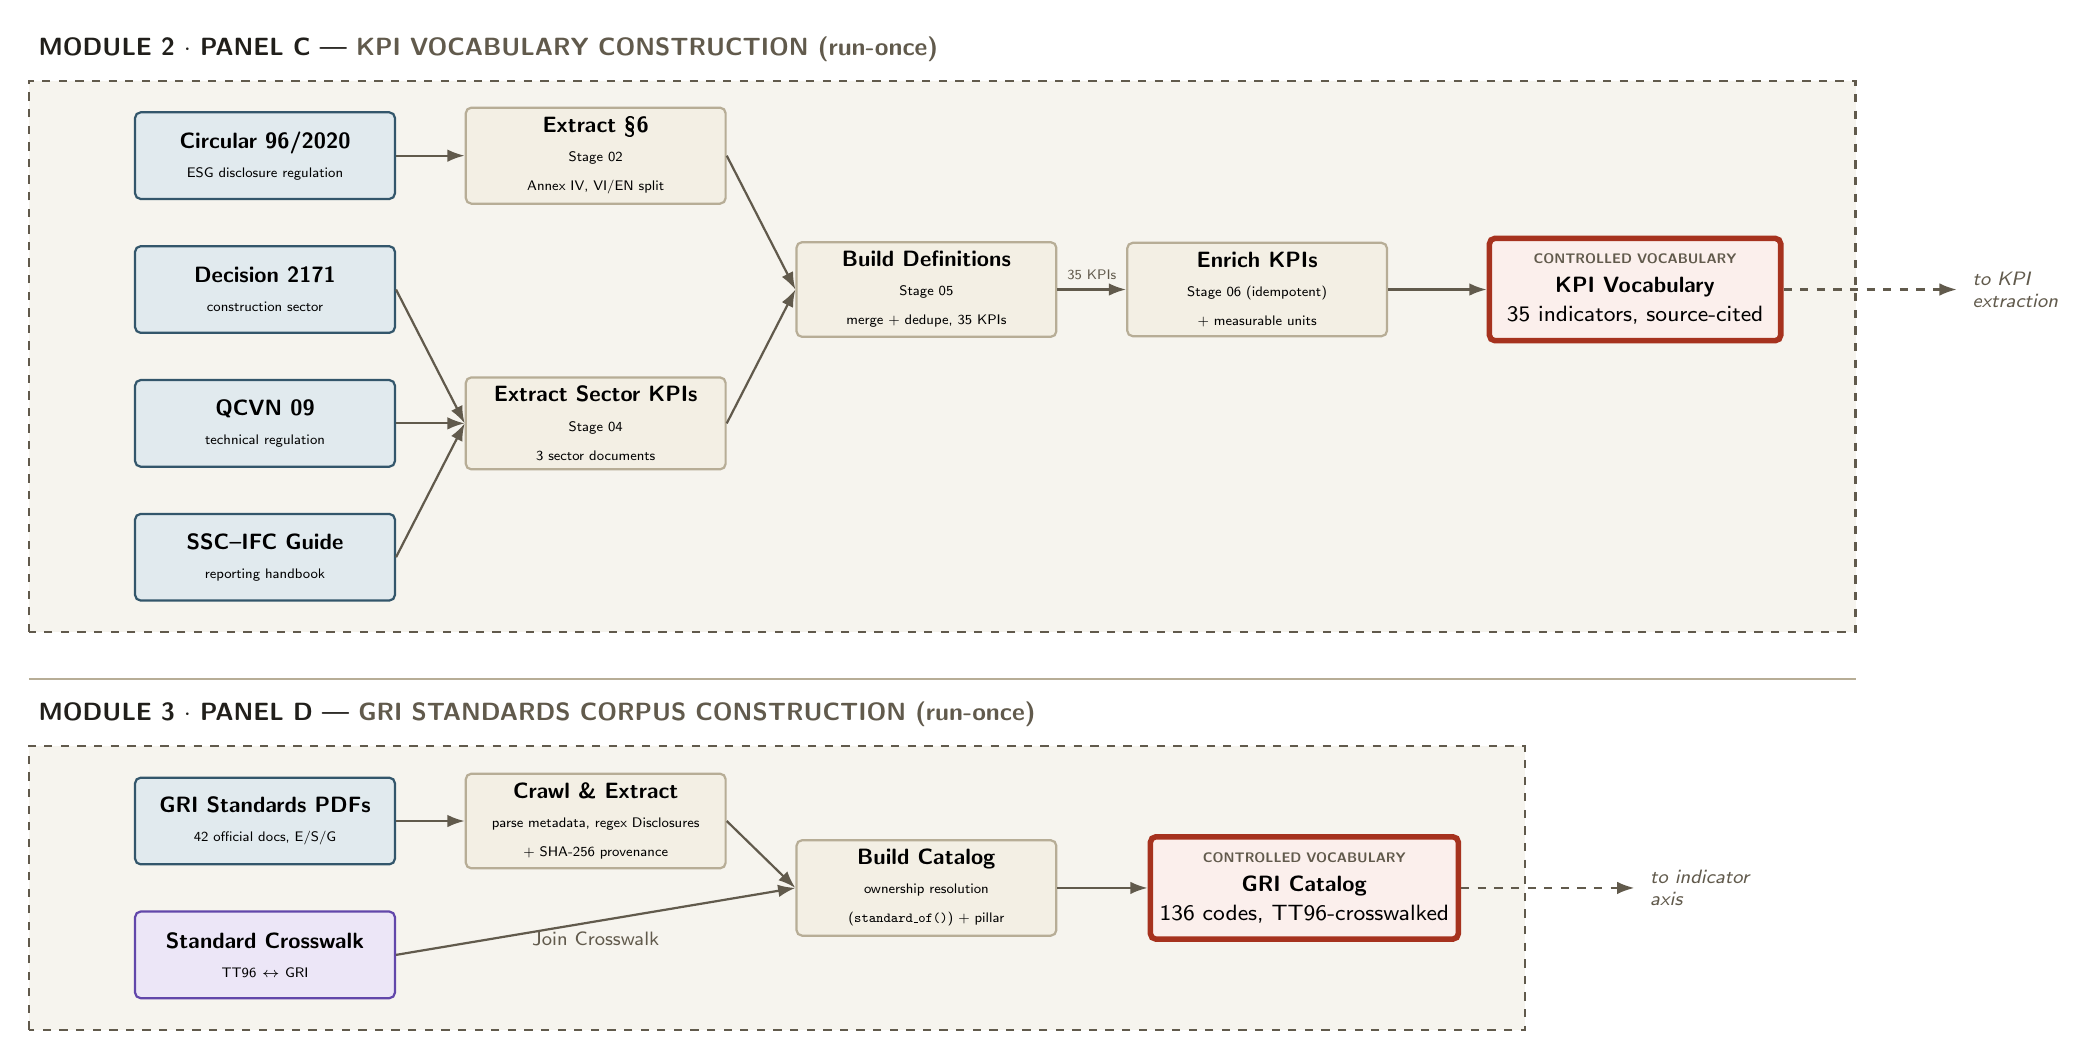
\begin{tikzpicture}[
    every node/.style={font=\sffamily},
    source/.style={rectangle, draw=pipsourceline, fill=pipsourcefill, rounded corners=2pt,
                   minimum width=3.3cm, minimum height=1.1cm, align=center,
                   font=\sffamily\footnotesize, line width=0.8pt},
    block/.style ={rectangle, draw=pipnodeline, fill=pipnodefill, rounded corners=2pt,
                   minimum width=3.3cm, minimum height=1.1cm, align=center,
                   font=\sffamily\footnotesize, line width=0.8pt},
    cfg/.style   ={rectangle, draw=pipconfigline, fill=pipconfigfill, rounded corners=2pt,
                   minimum width=3.3cm, minimum height=1.1cm, align=center,
                   font=\sffamily\footnotesize, line width=0.8pt},
    final/.style ={rectangle, draw=pipcontrib, fill=pipoutfill, rounded corners=2pt,
                   minimum width=3.7cm, minimum height=1.3cm, align=center,
                   font=\sffamily\footnotesize, line width=2.0pt},
    flow/.style={-{Latex[length=2.2mm, width=1.6mm]}, color=pipinksoft, line width=0.8pt},
    flowd/.style={flow, dashed},
    lbl/.style={font=\sffamily\scriptsize, color=pipinksoft},
    lblt/.style={font=\sffamily\scriptsize\itshape, color=pipinksoft},
    lane/.style={font=\sffamily\bfseries\small, color=pipink},
  ]

  \node[lane, anchor=west] at (-3.0,-4.60)
    {MODULE 2 $\cdot$ PANEL C --- \textcolor{pipinksoft}{KPI VOCABULARY CONSTRUCTION (run-once)}};

  \draw[pipinksoft, dashed, line width=0.8pt, fill=pipdpanelfill]
    (-3.0,-12.00) rectangle (20.2,-5.00);

  \node[source] (C1) at (0,-5.95) {\textbf{Circular 96/2020}\\[1pt]\tiny ESG disclosure regulation};
  \node[source] (C2) at (0,-7.65) {\textbf{Decision 2171}\\[1pt]\tiny construction sector};
  \node[source] (C3) at (0,-9.35) {\textbf{QCVN 09}\\[1pt]\tiny technical regulation};
  \node[source] (C4) at (0,-11.05) {\textbf{SSC--IFC Guide}\\[1pt]\tiny reporting handbook};

  \node[block] (CEXT1) at (4.2,-5.95)
    {\textbf{Extract \S6}\\[1pt]\tiny Stage 02\\[1pt]\tiny Annex IV, VI/EN split};
  \node[block] (CEXT2) at (4.2,-9.35)
    {\textbf{Extract Sector KPIs}\\[1pt]\tiny Stage 04\\[1pt]\tiny 3 sector documents};
  \node[block] (CMERGE) at (8.4,-7.65)
    {\textbf{Build Definitions}\\[1pt]\tiny Stage 05\\[1pt]\tiny merge + dedupe, 35 KPIs};
  \node[block] (CENR) at (12.6,-7.65)
    {\textbf{Enrich KPIs}\\[1pt]\tiny Stage 06 (idempotent)\\[1pt]\tiny + measurable units};
  \node[final] (COUT) at (17.4,-7.65)
    {\pitag{CONTROLLED VOCABULARY}\\[1pt]\textbf{KPI Vocabulary}\\[1pt]\footnotesize 35 indicators, source-cited};

  \draw[flow] (C1.east) -- (CEXT1.west);
  \draw[flow] (C2.east) -- (CEXT2.west);
  \draw[flow] (C3.east) -- (CEXT2.west);
  \draw[flow] (C4.east) -- (CEXT2.west);
  \draw[flow] (CEXT1.east) -- (CMERGE.west);
  \draw[flow] (CEXT2.east) -- (CMERGE.west);
  \draw[flow] (CMERGE.east) -- (CENR.west) node[lbl, midway, above] {\tiny 35 KPIs};
  \draw[flow] (CENR.east) -- (COUT.west);

  \draw[flowd] (COUT.east) -- ++(2.2,0)
    node[lblt, anchor=west, xshift=2pt, align=left] {to KPI\\extraction};

  \draw[pipnodeline, line width=0.6pt] (-3.0,-12.60) -- (20.2,-12.60);
  \node[lane, anchor=west] at (-3.0,-13.05)
    {MODULE 3 $\cdot$ PANEL D --- \textcolor{pipinksoft}{GRI STANDARDS CORPUS CONSTRUCTION (run-once)}};

  \draw[pipinksoft, dashed, line width=0.8pt, fill=pipdpanelfill]
    (-3.0,-17.05) rectangle (16.0,-13.45);

  \node[source] (G1) at (0,-14.40)   {\textbf{GRI Standards PDFs}\\[1pt]\tiny 42 official docs, E/S/G};
  \node[cfg]    (G2) at (0,-16.10)   {\textbf{Standard Crosswalk}\\[1pt]\tiny TT96 $\leftrightarrow$ GRI};
  \node[block]  (CRAWL) at (4.2,-14.40)
    {\textbf{Crawl \& Extract}\\[1pt]\tiny parse metadata, regex Disclosures\\[1pt]\tiny + SHA-256 provenance};
  \node[block]  (BUILD) at (8.4,-15.25)
    {\textbf{Build Catalog}\\[1pt]\tiny ownership resolution\\[1pt]\tiny (\texttt{standard\_of()}) + pillar};
  \node[final]  (GOUT) at (13.2,-15.25)
    {\pitag{CONTROLLED VOCABULARY}\\[1pt]\textbf{GRI Catalog}\\[1pt]\footnotesize 136 codes, TT96-crosswalked};

  \draw[flow] (G1.east) -- (CRAWL.west);
  \draw[flow] (CRAWL.east) -- (BUILD.west);
  \draw[flow] (G2.east) -- (BUILD.west) node[lbl, midway, below] {Join Crosswalk};
  \draw[flow] (BUILD.east) -- (GOUT.west);

  \draw[flowd] (GOUT.east) -- ++(2.2,0)
    node[lblt, anchor=west, xshift=2pt, align=left] {to indicator\\axis};

  \end{tikzpicture}%
  }
  \caption[Reference-corpus construction: KPI vocabulary and GRI catalogue]{Reference-corpus
    construction: two run-once, offline paths building the controlled
    vocabulary consumed downstream.}
  \label{fig:reference-corpus}
\end{figure}

\textbf{KPI vocabulary.} Four Vietnamese regulatory instruments --- Circular
96/2020/TT-BTC, Decision 2171/QĐ-BTC, QCVN 09:2013/BXD and the SSC--IFC ESG
reporting guide --- are downloaded and their relevant provisions extracted
\textit{verbatim} in two parallel passes: Circular 96's Section~6 (the
annual-report template's ESG-disclosure annex, in eight sub-sections) is
parsed for its Vietnamese/English indicator pairs, while the three
sector-specific sources are parsed for the non-fired building-materials
target, the energy-efficiency compliance clause and the SSC--IFC guide's
fourteen recommended aspects. The two extractions are merged and
deduplicated by indicator id into 35 KPI definitions, each carrying only the
source's verbatim wording and a source block naming the instrument, clause
and page. A final enrichment pass then attaches a short label and a
measurable definition with unit and normalisation hints to every indicator
--- since the regulations state \textit{topics to disclose}, not
\textit{metrics to measure}, and several extracted rows (e.g.\ ``Tái chế'')
are too thin on their own to drive numeric extraction --- while preserving
the original verbatim text in a \texttt{source.excerpt} field for audit. The
pass is idempotent: re-running it re-applies the same curated map without
overwriting the captured verbatim.

\textbf{GRI catalogue.} In parallel, 42 official GRI Standards PDFs are
linearised into one JSON file per standard, carrying the standard's own
metadata (parsed from its filename) and its disclosures (extracted by a
regular-expression scan for \texttt{Disclosure \emph{N}-\emph{n}} headings),
plus a SHA-256 of the source PDF for provenance. Building the catalogue is
not a plain merge: several standards --- the sector standards GRI~11--14 and
the 2024/25 rewrites GRI~101--103 --- re-list disclosures that belong to
other standards, so a disclosure is attributed to the one standard whose id
is its own prefix, not to whichever file is read first. This is not a
hypothetical failure mode: an earlier version that simply read files in
sorted filename order mis-attributed 80 of the eventual 136 entries, since
\texttt{"gri\_101"} sorts before \texttt{"gri\_2"} and so GRI~2-27 was
published under GRI~101's title, PDF and version. The corrected pass
produces 136 disclosure codes, each joined to a hand-curated TT96
$\leftrightarrow$ GRI crosswalk of which only explicitly confirmed rows are
used.

Because this corpus changes only when the standards themselves change, both
paths are built once, committed to version control alongside the source
PDFs and their SHA-256 digests, and treated thereafter as generated data.
How the two vocabularies join into the graph's indicator axis is described
in the Methodology chapter, and its yield is measured in an ablation later
in this thesis.


\subsection{Final packaging and distribution}
\label{sec:packaging}

Sentences are stored as JSONL, one record per sentence, carrying the
traceability triple, the text, the full probability vector, the thresholded
labels and channel-specific fields (article URL, domain, publication date
and crawl channel for news). Generated data is distributed through a
dataset repository rather than Git; the pushed revision is pinned in a
version file that \textit{is} tracked in Git, so a checkout recovers the
data that went with that code --- which is what makes the before/after
ablations reported later in this thesis reproducible rather than merely
asserted.
\section{Exploratory Data Analysis}
\label{sec:eda}


This section reports the exploratory analysis of the corpus, placed before
the methodology because several design decisions in
Chapter~\ref{ch:methodology} respond directly to properties measured here.
Every figure and table below is produced by
\texttt{docs/eda\_out/eda\_report\_data.py}, streaming the corpus directly
from disk.

The scope is the data only --- raw filings, derived sentences, ESG
annotation, temporal spread, conduct-channel composition --- not what the
pipeline subsequently \textit{produces} from it (KPI records, triples, the
resolved graph), which is a result rather than an input (\S\ref{sec:not-dataset})
and is measured later, in the Experiment chapter.


\subsection{Scale and coverage of the raw corpus}
\label{sec:eda-scale}
\begin{figure}[htbp]
  \centering
  \includegraphics[width=\linewidth]{fig_raw_corpus.png}
  \caption[Raw report corpus]{Raw report corpus. (a) Distribution of
    documents held per company. (b) Temporal spread, by the reporting
    year recoverable from the file name.}
  \label{fig:raw-corpus}
\end{figure}
Figure~\ref{fig:raw-corpus}(a) shows coverage per company is uneven but
rarely thin, with a mean of 12.3 documents per company across 115 companies.
Panel (b) shows the corpus thickening markedly over time; two causes are
confounded here and cannot be separated from file counts alone --- listed
companies genuinely publishing more, and recent filings simply being easier
to retrieve from public sources. Either way the consequence is the same:
evidence density is a function of year, and any comparison across years must
account for it rather than assume a stationary corpus.
\subsection{Sentence-level properties}
\label{sec:eda-sentence}

\begin{figure}[htbp]
  \centering
  \includegraphics[width=\linewidth]{fig_length_confidence.png}
  \caption[Sentence-level properties of the labelled report corpus]{%
    Sentence-level properties of the labelled report corpus.
    (a) Sentence-length distribution, with the ESG-classified subset
    overlaid. (b) Distribution of the highest pillar probability per
    sentence, against the 0.5 decision threshold.}
  \label{fig:sentence-properties}
\end{figure}

Parsing and segmentation produced 873,756 sentences from 1,216 documents
spanning 89,731 pages, a mean of 73.8 pages per document.
Figure~\ref{fig:sentence-properties}(a) shows the resulting length
distribution: the mean sentence length is 196 characters and the longest is
11,827 --- not a sentence at all but a table flattened into one text run by
the positional extractor, the clearest single artefact of the extraction
choice discussed in \S\ref{sec:cleaning}.

Figure~\ref{fig:sentence-properties}(b) is the more consequential view: the
distribution of the highest pillar probability is strongly bimodal, with
mass concentrated near 0 and near 1 and little in between. A classifier
whose scores concentrate at the extremes is confident, not necessarily
correct, and the two must not be conflated. What the distribution does
constrain is this: the 0.5 threshold is not cutting through a dense region,
so small threshold changes will not move the label counts much --- but it
says nothing about whether the confident decisions are right, which only the
evaluation table requested in \S\ref{sec:annotation} can answer.


\subsection{ESG label distribution and a precision concern}
\label{sec:eda-labels}
\begin{figure}[htbp]
  \centering
  \includegraphics[width=\linewidth]{fig_label_distribution.png}
  \caption[ESG annotation of the report corpus]{ESG annotation of the
    report corpus, scoped to the 282,195 sentences that carry at least
    one pillar label. (a) Frequency of each pillar; a sentence may carry
    several, so the bars do not sum to the total. (b) Every label
    combination that occurs, single-pillar against multi-label, on a log
    axis. The unlabelled remainder is excluded from both panels
    (Table~\ref{tab:esg-annotation}).}
  \label{fig:esg-annotation}
\end{figure}
\begin{table}[htbp]
  \centering \small
  \caption[ESG annotation of the report corpus]{ESG annotation of the
    report corpus. Pillar shares are taken over the pillar-labelled
    subset, not the whole corpus.}
  \label{tab:esg-annotation}
  \begin{tabularx}{\linewidth}{|L{1.473}|R{0.709}|R{0.818}|}
    \hline
    \rowcolor{hdrbg}
    \multicolumn{1}{|c|}{\textbf{Quantity}} &
    \multicolumn{1}{c|}{\textbf{Sentences}} &
    \multicolumn{1}{c|}{\textbf{Share}} \\ \hline
    Total sentences & 873,756 & 100\% of corpus \\ \hline
    \textbf{Classified ESG-relevant} (\texttt{esg} flag) & \textbf{303,723} & \textbf{34.8\% of corpus} \\ \hline
    \textbf{Carrying $\geq$1 pillar label} & \textbf{282,195} & \textbf{32.3\% of corpus} \\ \hline
    Carrying no pillar label & 591,561 & 67.7\% of corpus \\ \hline
    - Governance & 136,585 & 48.4\% of labelled \\ \hline
    - Social & 76,232 & 27.0\% of labelled \\ \hline
    - Environmental & 70,896 & 25.1\% of labelled \\ \hline
    Carrying more than one label & 1,518 & 0.5\% of labelled \\ \hline
  \end{tabularx}
\end{table}
Table~\ref{tab:esg-annotation} records four findings, the last two of which
qualify the annotation quality.

\textbf{The two annotation rules disagree measurably.}
\S\ref{sec:annotation} explains that a pillar tag needs a sigmoid score of
0.45, while the \texttt{esg} flag is set by the Neutral score falling below
0.5 --- different tests that diverge in both directions on this corpus:
30,783 sentences (10.1\% of the ESG set) are flagged ESG-relevant with no
pillar label, and a further 9,255 carry a pillar label but are not flagged
ESG-relevant. Neither is a bug --- the first is intended behaviour for a
signal that splits across pillars, the second for a sentence that is
confidently neutral yet mentions one pillar in passing --- but the two
fields must never be used interchangeably. The pipeline respects this: page
selection for the expensive extraction stage keys on the \texttt{esg} flag
(\S\ref{sec:extraction}), while the evidence interface's pillar columns are
read from the indicator axis, not from these labels, as described in the
Evidence View UI design later in this thesis.

\textbf{Governance dominates.} Governance appears on 136,585 sentences
against 76,232 for Social and 70,896 for Environmental --- roughly
1.9$\times$ the environmental count --- consistent with a Vietnamese annual
report's structure, where board composition, shareholder structure, internal
control and related-party transactions are mandatory, lengthy sections and
environmental disclosure is comparatively short. The downstream effect is
direct: the claim side of the graph is governance-heavy while the conduct
side, as \S\ref{sec:eda-asymmetry} shows, is environmental-heavy, so the two
channels do not measure the same thing in the same proportion.

\textbf{The multi-label formulation is barely exercised.} Panel (b) of
Figure~\ref{fig:esg-annotation} makes this visible: on a log axis the three
single-pillar bars sit at $10^{4}$--$10^{5}$ while all three multi-label
bars sit below 1,200. Only 1,518 sentences, 0.5\% of the pillar-labelled
subset, carry more than one pillar, and Governance~+~Social (1,190) accounts
for 78\% of even that; Environmental~+~Governance, the combination one would
most expect in a disclosure about board-approved emission targets, occurs
119 times in nearly nine hundred thousand sentences. In practice the model
behaves as a single-label classifier --- which does not invalidate the
multi-label design, correct in principle and costless, but means it is not
currently exercised in practice, and no stronger claim is made for it here.

\textbf{The ESG rate of 34.8\% is implausibly high.} Roughly one sentence in
three of an entire annual report being ESG-relevant is inconsistent with
these documents' composition on inspection. The likely mechanism is
lexical: Vietnamese corporate language uses environmental and social
vocabulary in contexts that are not disclosures. A concrete instance is
checkable in this corpus: the legal name of one issuer is \textit{Công ty Cổ
phần Nhựa và Môi trường Xanh An Phát} --- literally \textit{An Phat Green
Environment and Plastics JSC}. The string \textit{môi trường xanh} (``green
environment'') appears in 655 sentences, 189 of them (28.9\%) labelled
Environmental, including bare title-page lines stating nothing but the
company's name.

That pattern alone does not account for the whole gap --- 189 sentences out
of 303,723 is negligible in total --- but it establishes the
\textit{mechanism}: a company name, slogan or department title can trigger a
pillar label on lexical grounds alone, and there is no reason that mechanism
is confined to one issuer's name. Quantifying its full extent requires the
labelled evaluation set requested in \S\ref{sec:annotation}; until then, the
ESG rate reported here should be read as an upper bound on ESG-relevant
content, and the downstream stages are designed on that assumption. The
response is described in \S\ref{sec:extraction}: the extraction stage never
treats an ESG label as evidence of anything, only as a cost-saving filter
over which pages are worth sending to an expensive model.


\subsection{Temporal coverage}
\label{sec:temporal-coverage}
\begin{figure}[htbp]
  \centering
  \includegraphics[width=\linewidth]{fig_temporal_coverage.png}
  \caption[Temporal coverage of the labelled report corpus]{Temporal
    coverage of the labelled report corpus, by reporting year, with the
    ESG-classified subset overlaid.}
  \label{fig:temporal-coverage}
\end{figure}

\begin{table}[htbp]
  \centering \small
  \caption[Temporal coverage of the labelled report corpus]{Temporal
    coverage of the labelled report corpus (odd years shown; all years
    appear in Figure~\ref{fig:temporal-coverage}).}
  \label{tab:temporal-coverage}
  \begin{tabularx}{\linewidth}{|L{1.053}|R{1.053}|R{1.053}|R{0.842}|}
    \hline
    \rowcolor{hdrbg}
    \multicolumn{1}{|c|}{\textbf{Reporting year}} &
    \multicolumn{1}{c|}{\textbf{Sentences}} &
    \multicolumn{1}{c|}{\textbf{ESG sentences}} &
    \multicolumn{1}{c|}{\textbf{ESG share}} \\ \hline
    2011 & 27,318 & 6,641 & 24.3\% \\ \hline
    2013 & 27,834 & 7,588 & 27.3\% \\ \hline
    2015 & 26,889 & 8,369 & 31.1\% \\ \hline
    2017 & 52,215 & 17,093 & 32.7\% \\ \hline
    2019 & 68,579 & 23,048 & 33.6\% \\ \hline
    2021 & 69,678 & 25,877 & 37.1\% \\ \hline
    2023 & 72,222 & 27,518 & 38.1\% \\ \hline
    2025 & 99,172 & 38,331 & 38.7\% \\ \hline
  \end{tabularx}
\end{table}

Figure~\ref{fig:temporal-coverage} and Table~\ref{tab:temporal-coverage} plot
this by reporting year: the corpus spans 2008--2026, sentence volume rises
roughly fourfold across the period, and the ESG share rises with it, from
24.3\% to 38.7\%. The rise is gradual, not a step change --- notable because
Circular 96/2020 took effect in 2020, and a disclosure mandate that bound
immediately should show as a discontinuity that year. It does not.

Three explanations are consistent with a gradual rise, and the corpus
cannot distinguish between them: genuine secular growth in ESG disclosure
independent of the mandate, gradual compliance ramp-up rather than
immediate adoption, or drift in the vocabulary the classifier keys on with
no change in underlying content. The third would be a measurement artefact,
not a finding, and cannot be excluded without the evaluation set of
\S\ref{sec:annotation}. The claim made here is therefore restricted to what
the data supports: ESG-classified content grows as a share of the corpus
over time, and that growth is not attributable to the 2020 mandate on the
evidence available.


\subsection{The independent conduct channel}
\label{sec:eda-conduct}
\begin{figure}[htbp]
  \centering
  \includegraphics[width=\linewidth]{fig_news_sources.png}
  \caption[The conduct channel]{The conduct channel. (a) Source
    concentration across the twelve most frequent domains.
    (b) Distribution of stated publication year.}
  \label{fig:conduct-channel}
\end{figure}

\begin{table}[htbp]
  \centering \small
  \caption[Composition of the conduct channel]{Composition of the
    conduct channel.}
  \label{tab:conduct-channel}
  \begin{tabularx}{\linewidth}{|L{1.346}|R{0.654}|}
    \hline
    \rowcolor{hdrbg}
    \multicolumn{1}{|c|}{\textbf{Quantity}} &
    \multicolumn{1}{c|}{\textbf{Value}} \\ \hline
    Tickers covered & 115 \\ \hline
    Articles retrieved & 4,537 \\ \hline
    Sentences & 164,036 \\ \hline
    Mean articles per ticker & 39.5 \\ \hline
    Mean sentences per article & 36.2 \\ \hline
    \textbf{Distinct source domains} & \textbf{662} \\ \hline
    Share held by the three largest domains & 12.1\% \\ \hline
    Retrieved via Google News / Bing / DuckDuckGo & 3,398 / 1,113 / 26 \\ \hline
    Sentences explicitly mentioning the company & 35.9\% \\ \hline
    \textbf{Articles dated before 2010 (probable parse failures)} & \textbf{263 (5.8\%)} \\ \hline
  \end{tabularx}
\end{table}


\textbf{Independence is structurally sound.} Figure~\ref{fig:conduct-channel}(a) shows the twelve most frequent domains: the 4,537 articles come from 662
distinct domains, and the three largest --- \texttt{tinnhanhchungkhoan.vn},
\texttt{baodautu.vn}, \texttt{tapchicongthuong.vn} --- account for only
12.1\% of the corpus. This fragmented source distribution is the channel's
most favourable property: no single outlet's editorial position can
dominate the conduct side, though the corpus is still concentrated in
financial and business media rather than, say, environmental or local
reporting, which bounds the \textit{kind} of conduct it can observe.

\textbf{Retrieval is dominated by one back-end.} Of the three search
back-ends (Table~\ref{tab:conduct-channel}), one provider supplies roughly
three-quarters of the corpus, far more than the three-back-end design --- a
hedge against single-provider ranking bias --- was meant to allow. This is a
limitation of the corpus as built, not of the design, and is recorded as
such in the Discussion chapter.

\textbf{Severe recency skew.} Figure~\ref{fig:conduct-channel}(b) shows the
distribution of stated publication year: 3,103 of 4,507 dated articles
(68.8\%) were published in 2025 or 2026, so the conduct channel is
concentrated in the last two years while the claim channel spans fifteen.
This time asymmetry, on top of the volume asymmetry documented in
\S\ref{sec:eda-asymmetry}, is the direct cause of the asymmetric
retrieval-window design in the Methodology chapter's cross-check stage: a
claim made in 2012 has essentially no contemporaneous conduct evidence, so
the window must look forward, and far.

\textbf{Date quality is measurably imperfect.} The pre-2010 dates flagged in
Table~\ref{tab:conduct-channel} are not credible for a corpus of online
financial news about currently-listed issuers --- one value alone, 2002,
accounts for 179 of the 263, the signature of a template default rather
than a real date. These are extraction failures, not old articles, and are
left in the corpus rather than deleted, since the \texttt{date\_uncertain}
contract of \S\ref{sec:conduct-channel} exists precisely to carry this
uncertainty forward to the reader instead of hiding it. This measurement is
the empirical justification for that contract: without it, roughly one
article in seventeen would contribute a fabricated year to a temporal
graph.
\subsection{Claim--conduct asymmetry}
\label{sec:eda-asymmetry}
\begin{figure}[htbp]
  \centering
  \includegraphics[width=0.79\linewidth]{fig_claim_conduct_asymmetry.png}
  \caption[Volume and pillar asymmetry between the two channels]{Volume
    and pillar asymmetry between the two channels for the issuer
    analysed end-to-end. Note the logarithmic vertical axis.}
  \label{fig:channel-asymmetry}
\end{figure}

\begin{table}[htbp]
  \centering \small
  \caption[Claim channel versus conduct channel]{Claim channel versus
    conduct channel for the issuer analysed end-to-end.}
  \label{tab:claim-conduct-asymmetry}
  \begin{tabularx}{\linewidth}{|L{1.241}|R{1.034}|R{1.034}|R{0.69}|}
    \hline
    \rowcolor{hdrbg}
    \multicolumn{1}{|c|}{\textbf{Quantity}} &
    \multicolumn{1}{c|}{\textbf{Reports (claim)}} &
    \multicolumn{1}{c|}{\textbf{News (conduct)}} &
    \multicolumn{1}{c|}{\textbf{Ratio}} \\ \hline
    Sentences & 13,541 & 1,054 & 12.8$\times$ \\ \hline
    \textbf{ESG sentences} & \textbf{5,575} & \textbf{352} & \textbf{15.8$\times$} \\ \hline
    ESG share & 41.2\% & 33.4\% & - \\ \hline
    - Environmental & 1,207 & 297 & 4.1$\times$ \\ \hline
    - Social & 1,084 & 51 & 21.3$\times$ \\ \hline
    - Governance & 3,157 & 17 & 185.7$\times$ \\ \hline
  \end{tabularx}
\end{table}
Table~\ref{tab:claim-conduct-asymmetry} and Figure~\ref{fig:channel-asymmetry} state the central empirical constraint
on the entire system, conditioning every cross-check result reported in the
Experiment chapter: for the issuer analysed end to end, there is roughly one
piece of independent conduct evidence for every sixteen ESG claims, before
any consideration of whether the two are even about the same topic.

\textbf{The pillar composition also inverts.} Governance is the largest
pillar in reports and the smallest in news; Environmental is the reverse
(Table~\ref{tab:claim-conduct-asymmetry}), so the governance ratio (186:1)
is far more extreme than the environmental ratio (4.1:1).

This has a specific implication: independent media write about factories,
emissions and environmental incidents, not a company's internal control
framework, so a governance claim is structurally far less checkable than an
environmental one in this corpus --- not because governance claims are
harder to evaluate in principle, but because no independent party produces
evidence about them. Since the claim side is governance-heavy and the
conduct side is environmental-heavy, the two channels are least aligned
exactly where claim volume is greatest; this is the structural reason for
the large unverified count in the Experiment chapter's cross-check results,
a property of the evidence environment rather than a defect of the matching
algorithm.


\subsection{What the exploration implies for the design}
\label{sec:eda-implications}

Five properties measured above drive design decisions in
Chapter~\ref{ch:methodology}, collected here so the connection is explicit
rather than implied.

\begin{enumerate}
  \item \textbf{The conduct channel is $\sim$15.8$\times$ smaller than the
    claim channel and inverted in pillar composition}
    (\S\ref{sec:eda-asymmetry}). Consequence: the system must be able to return
    \textit{``not verifiable''} as a first-class outcome rather than forcing a
    verdict. This is why the cross-check emits three assessments, one of which
    is \texttt{unverified\_insufficient\_evidence}
    (\S\ref{sec:problem-definition}).

  \item \textbf{The conduct channel is concentrated in the last two years while
    claims span fifteen} (\S\ref{sec:eda-conduct}). Consequence: the retrieval
    window is deliberately asymmetric --- one year backward, fifty forward, a
    design specified in the Methodology chapter's cross-check stage.

  \item \textbf{5.8\% of articles carry an implausible publication date}
    (\S\ref{sec:eda-conduct}). Consequence: the \texttt{date\_uncertain} flag
    is mandatory on news-derived observations and is propagated into every
    dossier as a visible caveat (\S\ref{sec:conduct-channel}), a contract
    honoured throughout the cross-check stage described in the Methodology
    chapter.

  \item \textbf{The ESG classifier's 34.8\% positive rate is an upper bound,
    with a demonstrated lexical failure mode} (\S\ref{sec:eda-labels}).
    Consequence: the ESG label is used only as a cost filter over which pages
    to send to an expensive extractor, never as evidence in its own right
    (\S\ref{sec:extraction}).

  \item \textbf{79.5\% of extracted KPI occurrences fall outside the controlled
    vocabulary and units are written 189 different ways}, a KPI-yield result
    reported in the Experiment chapter. Consequence: canonicalisation is a
    separate offline stage that writes a \textit{new} property rather than
    overwriting the raw one, and rejects rather than force-maps ambiguous
    cases, as described in the Methodology chapter's Validate \& Normalize
    stage.
\end{enumerate}
\chapter{Methodology}
\label{ch:methodology}
\section{Problem Definition}
\label{sec:problem-definition}

This section fixes the task the rest of the chapter operationalises, so \textsf{supports}, \textsf{contradicts} and \textsf{unverified} carry one meaning throughout, and what the system does not do is legible as a scope decision, not an omission a reader discovers on close reading.

Let $O$ be the set of issuers (companies) in the corpus. A \emph{sustainability claim} is a tuple $c = (o_c, \tau_c, \pi_c)$: $o_c \in O$ is the issuing organisation, $\tau_c$ is the interval over which the claim asserts something to be or become true (\texttt{valid\_from}/\texttt{valid\_to}, defaulting to the report's fiscal year when no explicit horizon is stated), and $\pi_c$ is its provenance --- the (document, page, sentence) triple it was extracted from. $C$ is the set of all claims; every $c \in C$ carries \texttt{source\_type = report}, since a claim is by definition something a company said about itself.

Let $E$ be the set of \emph{conduct evidence}: instances of the graph's news-derived observation classes (\texttt{KPIObservation}, \texttt{Controversy}, \texttt{Penalty}, \texttt{MediaReport}), each stamped \texttt{source\_type = news} and each a tuple $e = (o_e, \tau_e, \pi_e)$ in the same shape as a claim. $E$ is drawn from a corpus collected independently of the companies under study --- the independent conduct channel introduced in Chapter 2 as this thesis's second contribution; this independence, not any property of the adjudication step below, is what lets conduct evidence falsify a claim rather than merely restate it.

For a claim $c$, retrieval selects a candidate set $R(c) \subseteq E$ of conduct evidence sharing $c$'s resolved issuer and temporally compatible with $\tau_c$ --- made possible by the graph's entity resolution and temporal metadata, rather than a full cross-product search over every claim and every article. An \emph{adjudication function}
\[
  f : C \times E \rightarrow \{\textsf{supports}, \textsf{contradicts}, \textsf{irrelevant}\}
\]
is applied to every pair $(c, e)$ with $e \in R(c)$, specified later in this chapter as a prompted LLM judgement over retrieved evidence, not a learned classifier. Claim-level status is then the aggregate
\[
  g(c) =
  \begin{cases}
    \textsf{contradicted} & \text{if } \exists\, e \in R(c) : f(c,e) = \textsf{contradicts} \\
    \textsf{supported}    & \text{if no such } e \text{ exists, and } \exists\, e \in R(c) : f(c,e) = \textsf{supports} \\
    \textsf{unverified}   & \text{otherwise } (R(c) = \emptyset\text{, or every } f(c,e) = \textsf{irrelevant})
  \end{cases}
\]
Contradiction dominates support by construction: a single credible counter-example is informative even alongside corroborating evidence, while the absence of a counter-example proves nothing. \textsf{Unverified} deliberately collapses two situations a reader might want distinguished --- no candidate evidence existed for $c$, versus candidate evidence existed but was judged irrelevant --- into one label, since both mean the same thing operationally: the pipeline has nothing that speaks against the claim, which is not the same as confirming it.

What is explicitly \emph{not} defined is any function $h : C \rightarrow [0,1]$. Composing $g$ into such a score is technically straightforward, and was deliberately not done: no ground-truth greenwashing label exists for this corpus, or for any Vietnamese corpus, against which $h$ could be fit or validated. Returning $g(c)$ with the evidence and provenance that produced it, and leaving the greenwashing judgement to the reader, is the scope boundary this thesis holds to.

\section{System Architecture}
\begin{figure}[H]
  \centering
  \resizebox{0.98\linewidth}{!}{%
  \begin{tikzpicture}[
    every node/.style={font=\sffamily},
    source/.style={rectangle, draw=pipsourceline, fill=pipsourcefill, rounded corners=2pt,
                   align=center, line width=0.8pt, inner sep=3pt},
    block/.style ={rectangle, draw=pipnodeline, fill=pipnodefill, rounded corners=2pt,
                   align=center, line width=0.8pt, inner sep=3pt},
    final/.style ={rectangle, draw=pipink, fill=pipnodefill, rounded corners=2pt,
                   align=center, line width=1.6pt, inner sep=3pt},
    finalsrc/.style={final, fill=pipsourcefill},
    config/.style ={rectangle, draw=pipconfigline, fill=pipconfigfill, rounded corners=2pt,
                   align=center, line width=1.0pt, inner sep=3pt},
    model/.style ={rectangle, draw=pipmodelline, fill=pipmodelfill, rounded corners=3pt,
                   align=center, line width=1.5pt, inner sep=3pt},
    contrib/.style={draw=pipcontrib, line width=2.2pt},
    contribd/.style={rectangle, draw=pipcontrib, fill=white, dashed, rounded corners=2pt,
                   align=center, line width=1.3pt, inner sep=3pt},
    flow/.style={-{Latex[length=2mm, width=1.5mm]}, color=pipinksoft, line width=0.7pt},
    flowd/.style={flow, dashed},
    wrap/.style={-{Latex[length=2mm, width=1.5mm]}, color=pipink, line width=0.9pt},
    lbl/.style={font=\sffamily\tiny, color=pipinksoft},
    lane/.style={font=\sffamily\bfseries\scriptsize, color=pipink},
  ]


  \node[lane, anchor=west] at (-2.5,6.15)
    {MODULE 0 --- \textcolor{pipinksoft}{KPI VOCABULARY CONSTRUCTION (run-once, offline --- detail in Figure~\ref{fig:reference-corpus})}};
  \draw[pipframeline, line width=0.7pt, rounded corners=4pt, fill=pipdpanelfill]
    (-2.6,4.15) rectangle (24.6,5.9);

  \node[source, minimum width=4.0cm, minimum height=1.0cm] (C1) at (0,5.0)
    {\textcolor{pipsourceline}{\faIcon{file-alt}}~\textbf{\scriptsize 4 Regulatory Documents}\\[1pt]\tiny Circular 96, Decision 2171, QCVN 09, SSC--IFC};
  \node[block, minimum width=3.6cm, minimum height=1.0cm] (CEXT) at (6.3,5.0)
    {\textcolor{pipnodeline}{\faCut}~\textbf{\scriptsize Extract \S6 + Sector KPIs}\\[1pt]\tiny Stages 2 \& 4};
  \node[block, minimum width=3.8cm, minimum height=1.0cm] (CMERGE) at (12.6,5.0)
    {\textcolor{pipnodeline}{\faObjectGroup}~\textbf{\scriptsize Merge, Dedupe \& Enrich}\\[1pt]\tiny Stages 5--6, 35 KPIs};
  \node[finalsrc, minimum width=3.8cm, minimum height=1.05cm] (COUT) at (19.0,5.0)
    {\pitag{CONTROLLED VOCABULARY}\\[1pt]\textcolor{pipink}{\faBook}~\textbf{\scriptsize KPI Vocabulary}\\[1pt]\tiny 35 indicators, source-cited};
  \draw[flow] (C1.east) -- (CEXT.west);
  \draw[flow] (CEXT.east) -- (CMERGE.west);
  \draw[flow] (CMERGE.east) -- (COUT.west);


  \node[lane, anchor=west] at (-2.5,2.4)
    {MODULE 1 --- \textcolor{pipinksoft}{DATA CONSTRUCTION $\to$ EXTRACTION $\to$ VALIDATE \& NORMALIZE}};
  \draw[pipframeline, line width=0.7pt, rounded corners=4pt, fill=pipdpanelfill]
    (-2.6,-1.6) rectangle (24.6,2.15);

  \node[source, minimum width=4.6cm, minimum height=1.15cm] (DC) at (0,0)
    {\textcolor{pipsourceline}{\faStream}~\textbf{\scriptsize Data Construction}\\[1pt]\tiny report + news ingestion, ESG classification\\[1pt]\tiny see Figure~\ref{fig:pipeline-overview}};

  \node[final, minimum width=2.9cm, minimum height=0.85cm] (A5) at (4.9,0.85)
    {\pitag{CLAIM SIDE}\\[1pt]\textcolor{pipink}{\faLayerGroup}~\textbf{\scriptsize ESG Claim Corpus}};
  \node[final, contrib, minimum width=2.9cm, minimum height=0.85cm] (B5) at (4.9,-0.85)
    {\pitag{CONDUCT $\bigstar$}\\[1pt]\textcolor{pipcontrib}{\faLayerGroup}~\textbf{\scriptsize ESG Conduct Corpus}};
  \draw[flow] (DC.east) -- ++(0.55,0) |- (A5.west);
  \draw[flow] (DC.east) -- ++(0.55,0) |- (B5.west);

  \node[model, minimum width=4.6cm, minimum height=1.15cm] (EXT) at (10.0,0)
    {\textcolor{pipmodelline}{\faRobot}~\textbf{\scriptsize Extraction}\\[1pt]\tiny LLM $\cdot$ KPI records + graph triples};
  \draw[flowd] (COUT.south) -- ++(0,-0.9) -| (EXT.north);
  \draw[flow] (A5.east) -- ++(0.55,0) |- (EXT.west);
  \draw[flow] (B5.east) -- ++(0.55,0) |- (EXT.west);

  \node[block, minimum width=4.6cm, minimum height=1.15cm] (VN) at (15.6,0)
    {\textcolor{pipnodeline}{\faWrench}~\textbf{\scriptsize Validate \& Normalize}\\[1pt]\tiny repair triples $\cdot$ canonicalize dates/units/ids};
  \draw[flow] (EXT.east) -- (VN.west);

  \node[finalsrc, minimum width=3.6cm, minimum height=0.95cm] (VT) at (20.6,0)
    {\textcolor{pipink}{\faIcon{list-alt}}~\textbf{\scriptsize Validated Triples}};
  \draw[flow] (VN.east) -- (VT.west);



  \node[lane, anchor=west] at (-2.2,-2.45)
    {MODULE 1.5 --- \textcolor{pipinksoft}{GRI CATALOGUE \& ISSUER REGISTRY CONSTRUCTION (run-once, offline $+$ human-in-the-loop)}};
  \draw[pipframeline, line width=0.7pt, rounded corners=4pt, fill=pipdpanelfill]
    (-2.3,-4.5) rectangle (25.2,-2.7);

  \node[source, minimum width=3.4cm, minimum height=0.85cm] (G1) at (0,-3.6)
    {\textcolor{pipsourceline}{\faIcon{file-alt}}~\textbf{\scriptsize 42 GRI Standards PDFs}\\[1pt]\tiny + hand-curated crosswalk};
  \node[block, minimum width=3.6cm, minimum height=1.0cm] (GBUILD) at (5.6,-3.6)
    {\textcolor{pipnodeline}{\faSitemap}~\textbf{\scriptsize Crawl, Extract \& Build Catalog}\\[1pt]\tiny \texttt{standard\_of()} ownership + pillar};
  \node[finalsrc, minimum width=3.4cm, minimum height=1.0cm] (GOUT) at (11.2,-3.6)
    {\pitag{CONTROLLED VOCABULARY}\\[1pt]\textcolor{pipink}{\faBook}~\textbf{\scriptsize GRI Catalog}\\[1pt]\tiny 136 codes, TT96-crosswalked};
  \draw[flow] (G1.east) -- (GBUILD.west);
  \draw[flow] (GBUILD.east) -- (GOUT.west);

  \node[block, minimum width=3.8cm, minimum height=1.05cm] (IDRAFT) at (17.0,-3.6)
    {\textcolor{pipnodeline}{\faAddressBook}~\textbf{\scriptsize Draft Issuer Aliases}\\[1pt]\tiny Stage 04: aliases / exclusions / \texttt{needs\_review}};
  \draw[wrap] (VT.south) -- ++(0,-1.725) -| (IDRAFT.north);

  \node[finalsrc, minimum width=3.6cm, minimum height=1.0cm] (IOUT) at (22.8,-3.6)
    {\textcolor{pipink}{\faUserCheck}~\textbf{\scriptsize Issuer Registry}\\[1pt]\tiny human confirms \texttt{needs\_review}};
  \draw[flow] (IDRAFT.east) -- (IOUT.west)
    node[lbl, midway, above, align=center] {\tiny human-in-\\\tiny the-loop};



  \node[lane, anchor=west] at (-3.4,-5.25)
    {MODULE 2 --- \textcolor{pipinksoft}{ENTITY RESOLUTION \& INDICATOR AXIS $\to$ GRAPH LOAD \& CROSS-CHECK}};
  \draw[pipframeline, line width=0.7pt, rounded corners=4pt, fill=pipdpanelfill]
    (-3.7,-11.25) rectangle (24.6,-6.8);

  \draw[pipconfigline, line width=0.6pt, rounded corners=3pt, fill=white]
    (-3.6,-10.35) rectangle (-0.2,-7.6);
  \node[anchor=north west, font=\sffamily\bfseries\tiny, text=pipconfigline] at (-3.55,-7.7)
    {ISSUER + STANDARDS REGISTRIES};
  \node[config, minimum width=3.0cm, minimum height=0.85cm] (REG) at (-1.9,-8.3)
    {\textcolor{pipconfigline}{\faAddressBook}~\textbf{\scriptsize Issuer Registry}};
  \node[config, minimum width=3.0cm, minimum height=0.85cm] (STD) at (-1.9,-9.7)
    {\textcolor{pipconfigline}{\faBalanceScale}~\textbf{\scriptsize Standards Registry}};

  \node[block, minimum width=5.7cm, minimum height=1.55cm] (ER) at (3.7,-8.5)
    {\textcolor{pipnodeline}{\faCogs}~\textbf{\scriptsize Entity Resolution \& Indicator Axis}\\[1pt]\tiny merge duplicates $\cdot$ stamp provenance\\[1pt]\tiny build the TT96 $\leftrightarrow$ GRI indicator axis};
  \draw[flowd] (GOUT.south) -- ++(0,-2.2) -| (ER.north);
  \draw[flowd] (IOUT.south) -- ++(0,-1.8) -| (REG.north);
  \draw[flow] (REG.east) -- (ER.west);
  \draw[flow] (STD.east) -- (ER.west);

  \node[finalsrc, minimum width=3.9cm, minimum height=1.0cm] (RG) at (9.7,-8.5)
    {\textcolor{pipink}{\faProjectDiagram}~\textbf{\scriptsize Resolved Graph}\\[1pt]\tiny the temporal ESG knowledge graph};
  \draw[flow] (ER.east) -- (RG.west);

  \node[contribd, minimum width=2.6cm, minimum height=1.35cm] (QA) at (9.7,-10.25)
    {\textcolor{pipcontrib}{\faClipboardCheck}~\textbf{\scriptsize $\bigstar$ Quality Audit}\\[1pt]\tiny label-free, run\\[1pt]\tiny before/after changes};
  \draw[pipcontrib, dashed, line width=0.9pt] (RG.south) -- (QA.north);

  \node[block, minimum width=2.9cm, minimum height=1.0cm] (GL) at (14.7,-7.65)
    {\textcolor{pipnodeline}{\faDatabase}~\textbf{\scriptsize Graph Load}\\[1pt]\tiny into Neo4j};
  \node[finalsrc, minimum width=2.8cm, minimum height=0.85cm] (GLOUT) at (18.6,-7.65)
    {\textcolor{pipink}{\faDatabase}~\textbf{\scriptsize Base Graph}\\[1pt]\tiny loaded};
  \draw[flow] (GL.east) -- (GLOUT.west);
  \node[model, contrib, minimum width=3.4cm, minimum height=1.25cm] (CC) at (14.7,-9.5)
    {\textcolor{pipcontrib}{\faRobot}~\textbf{\scriptsize Claim--Conduct}\\\textbf{\scriptsize Cross-Check $\bigstar$}\\[1pt]\tiny LLM: supports/contradicts/irrelevant};
  \draw[flow] (RG.east) -- ++(0.55,0) |- (GL.west);
  \draw[flow] (RG.east) -- ++(0.55,0) |- (CC.west);

  \node[finalsrc, minimum width=3.6cm, minimum height=0.85cm] (DOS) at (19.4,-9.5)
    {\textcolor{pipink}{\faFileContract}~\textbf{\scriptsize Claim Assessment Dossiers}};
  \draw[flow] (CC.east) -- (DOS.west);



  \node[lane, anchor=west] at (-1.9,-13.05)
    {MODULE 3 --- \textcolor{pipinksoft}{GRAPH LOAD \& ADVISORY SYNC $\to$ PRESENTATION}};
  \draw[pipframeline, line width=0.7pt, rounded corners=4pt, fill=pipdpanelfill]
    (-2.0,-16.2) rectangle (11.3,-13.3);

  \node[block, minimum width=3.4cm, minimum height=0.95cm] (AS) at (0,-14.7)
    {\textcolor{pipnodeline}{\faIcon{sync-alt}}~\textbf{\scriptsize Advisory Sync}\\[1pt]\tiny merges assessment dossiers in};
  \node[finalsrc, minimum width=2.6cm, minimum height=0.95cm] (NEO) at (4.2,-14.7)
    {\textcolor{pipink}{\faDatabase}~\textbf{\scriptsize Neo4j}\\[1pt]\tiny base + advisory};
  \draw[wrap] (DOS.south) -- ++(0,-1.5) -| (AS.north);
  \draw[wrap] (GLOUT.south) -- ++(0,-3.85) -| (NEO.north);
  \draw[flow] (AS.east) -- (NEO.west);

  \node[finalsrc, minimum width=3.4cm, minimum height=1.0cm] (LED) at (9.0,-14.1)
    {\textcolor{pipink}{\faClipboardList}~\textbf{\scriptsize Claim Ledger}\\[1pt]\tiny per company, Markdown};
  \node[finalsrc, minimum width=3.4cm, minimum height=1.0cm] (UI) at (9.0,-15.4)
    {\textcolor{pipink}{\faDesktop}~\textbf{\scriptsize Evidence View UI}\\[1pt]\tiny 3-column web demo};
  \draw[flow] (NEO.east) -- ++(0.5,0) |- (LED.west);
  \draw[flow] (NEO.east) -- ++(0.5,0) |- (UI.west);

  \end{tikzpicture}%
  }
  \caption[Full construction and analysis pipeline]{Full construction and
    analysis pipeline, redrawn as five stacked modules to fit the page
    width.}
  \label{fig:full-pipeline}
\end{figure}

Figure~\ref{fig:full-pipeline} gives the complete system architecture referred to throughout this chapter. Data construction is detailed in full in Figure~\ref{fig:pipeline-overview}, so it is condensed here into a single module producing the two evidence corpora; the two reference-construction modules (0 and 1.5) show inline how the KPI vocabulary, GRI catalogue and issuer registry that later stages depend on are each built; the temporal-knowledge-graph construction and claim--conduct cross-check pipeline that follows --- Extraction, Validate \& Normalize, Entity Resolution \& Indicator Axis, Graph Load, Claim--Conduct Cross-Check, Advisory Sync, and Presentation --- is what the rest of this chapter specifies one stage at a time. Blocks with a crimson border are this thesis's own contribution beyond the underlying EmeraldMind design; every other block is standard NLP or data-engineering machinery.

\section{Extraction}
\label{sec:extraction}

Extraction is the stage that turns one page of ESG-labelled text into two structured artefacts: a set of KPI records checked against the controlled indicator vocabulary built in Chapter 2, and a set of typed graph nodes and directed, temporally-scoped edges checked against the class and edge-label schema from Chapter 1. Both come from a single language-model call per page, restricted to pages with at least one ESG-relevant sentence, and both preserve the (document, page, sentence) provenance of every value they emit --- a property identity resolution, cross-checking and the final claim ledger all depend on downstream, since none of them re-reads the source document.

The two calls are not independent, and Figure~\ref{fig:extraction-detail} makes the dependency explicit: KPI extraction runs first, and its output is one of the inputs triple extraction receives, alongside the page text and the schema. This ordering matters because a KPI record is more constrained than a free-form triple --- it can only take the shape one of the 35 controlled indicators defines --- so resolving it first gives triple extraction a small, already-typed KPI observation to attach to an organisation, rather than asking one model call to invent both the indicator identity and the graph structure around it at once.

\begin{figure}[H]
  \centering
  \resizebox{0.78\linewidth}{!}{%
  \begin{tikzpicture}[
    every node/.style={font=\sffamily},
    source/.style={rectangle, draw=pipsourceline, fill=pipsourcefill, rounded corners=2pt,
                   align=center, line width=0.8pt, inner sep=3pt},
    config/.style ={rectangle, draw=pipconfigline, fill=pipconfigfill, rounded corners=2pt,
                   align=center, line width=1.0pt, inner sep=3pt},
    model/.style ={rectangle, draw=pipmodelline, fill=pipmodelfill, rounded corners=3pt,
                   align=center, line width=1.5pt, inner sep=3pt},
    final/.style ={rectangle, draw=pipink, fill=pipnodefill, rounded corners=2pt,
                   align=center, line width=1.6pt, inner sep=3pt},
    flow/.style={-{Latex[length=2mm, width=1.5mm]}, color=pipinksoft, line width=0.7pt},
    flowd/.style={flow, dashed},
    lbl/.style={font=\sffamily\tiny, color=pipinksoft},
  ]

  \node[source, minimum width=3.8cm, minimum height=1.0cm] (PAGE) at (0,-1.6)
    {\textcolor{pipsourceline}{\faIcon{file-alt}}~\textbf{\scriptsize ESG-Labelled Page}\\[1pt]\tiny gated on \(\geq\)1 ESG-relevant sentence};

  \node[config, minimum width=3.4cm, minimum height=0.95cm] (VOC) at (0,-4.0)
    {\textcolor{pipconfigline}{\faBook}~\textbf{\scriptsize KPI Vocabulary}\\[1pt]\tiny 35 controlled indicators};

  \node[model, minimum width=5.6cm, minimum height=1.15cm] (KEX) at (5.2,-1.6)
    {\textcolor{pipmodelline}{\faRobot}~\textbf{KPI Extraction}\\[1pt]\tiny LLM $\cdot$ one call per page};

  \draw[flow] (PAGE.east) -- (KEX.west);
  \draw[flowd] (VOC.east) -- (2.7,-4.0) -- (2.7,-2.175);

  \node[final, minimum width=4.4cm, minimum height=1.05cm] (KREC) at (5.2,-4.0)
    {\textcolor{pipink}{\faTable}~\textbf{\scriptsize KPI Records}\\[1pt]\tiny value $\cdot$ unit $\cdot$ kind $\cdot$ year $\cdot$ snippet};
  \draw[flow] (KEX.south) -- (KREC.north);

  \node[config, minimum width=3.4cm, minimum height=0.95cm] (SCH) at (11.6,-4.0)
    {\textcolor{pipconfigline}{\faCode}~\textbf{\scriptsize Graph Schema}\\[1pt]\tiny node classes, edge labels};

  \node[model, minimum width=5.6cm, minimum height=1.15cm] (TEX) at (11.6,-1.6)
    {\textcolor{pipmodelline}{\faRobot}~\textbf{Triple Extraction}\\[1pt]\tiny LLM $\cdot$ one call per page};

  \draw[flow] (KREC.east) -- (TEX.south west);
  \draw[flow] (PAGE.east) -- (1.9,-0.75) -- (8.8,-0.75) -- (TEX.west);
  \draw[flowd] (SCH.north) -- (TEX.south);

  \node[final, minimum width=5.6cm, minimum height=1.15cm] (OUT) at (11.6,1.0)
    {\textcolor{pipink}{\faProjectDiagram}~\textbf{\scriptsize Typed Nodes + Temporal Edges}\\[1pt]\tiny stamped \texttt{source\_type}, provenance};
  \draw[flow] (TEX.north) -- (OUT.south);
  \draw[flowd] (OUT.east) -- +(1.6,0) node[lbl, anchor=west, xshift=2pt, font=\sffamily\scriptsize\itshape, align=left]
    {to Validate \& Normalize};

  \end{tikzpicture}%
  }
  \caption[Extraction, detailed]{Extraction, detailed --- internal structure
    of the \emph{Extraction} block in Figure~\ref{fig:full-pipeline}.}
  \label{fig:extraction-detail}
\end{figure}

A single worked example fixes what these two calls actually produce. Page 31 of one 2024 annual report in the corpus follows a table of environmental-compliance figures with the sentence:
\begin{quote}
  \emph{"Không có sai phạm về vấn đề môi trường xảy ra trong năm."}\\
  (No environmental violations occurred during the year.)
\end{quote}
This sentence matches the controlled indicator for the number of environmental-compliance penalties incurred in the reporting period. Table~\ref{tab:extraction-example} shows what each of the two calls emits for it.

\begin{table}[htbp]
  \centering \small
  \caption[Extraction output for one worked example]{What KPI extraction and
    triple extraction each emit for the sentence above.}
  \label{tab:extraction-example}
  \begin{tabularx}{\linewidth}{|L{0.6}|L{1.4}|}
    \hline
    \rowcolor{hdrbg}
    \multicolumn{1}{|c|}{\textbf{Field}} &
    \multicolumn{1}{c|}{\textbf{Extracted value}} \\ \hline
    Indicator & Number of times penalised for environmental non-compliance in the reporting period \\ \hline
    Value / unit / kind & 0 / times / achieved \\ \hline
    Reporting year & 2024 \\ \hline
    Snippet (verbatim anchor) & "Không có sai phạm về vấn đề môi trường xảy ra trong năm." \\ \hline
    Node produced & one \texttt{KPIObservation} node carrying the fields above, plus a validity interval covering the 2024 reporting period \\ \hline
    Edge produced & the reporting organisation \(\rightarrow\) that observation, carrying its own temporal metadata (\texttt{valid\_from}, \texttt{valid\_to}, \texttt{recorded\_at}) separate from either node's \\ \hline
    Stamp on both node and edge & \texttt{source\_type = report} \\ \hline
  \end{tabularx}
\end{table}

Read in isolation, this is an entirely unremarkable, self-reported compliance record. It is also exactly the kind of record the independent conduct channel exists to check: a company has every incentive to report zero penalties whether or not one occurred, and nothing available to this stage --- the page text, the indicator vocabulary, the schema --- can tell an actually clean record apart from an unreported one. Extraction stays deliberately silent on that question, carrying a self-reported zero forward as a claim like any other; it is the cross-check later in this chapter, matching it against evidence this stage never sees, that is positioned to distinguish the two.

\section{Validate \& Normalize}
\label{sec:validate-normalize}

Extraction is one language-model call per page, so nothing in it sees the graph as a whole: two pages can invent slightly different spellings of the same edge label, a temporal field can be left off, or the reversed direction of a legal (source class, target class) pair can slip through. Validate \& Normalize closes that gap before any node is merged or resolved --- it never touches the graph's identity or structure, only whether every extracted triple is schema-legal and every date on it means the same thing everywhere else in the corpus. It runs three passes over the same triple set: a repair pass corrects and temporally normalizes what extraction produced, an anchoring pass adds structural links the extraction prompt could not always infer, and a canonicalization pass places every KPI observation into the 35-indicator controlled vocabulary. The three run as a single unit that reads the triples once and writes the validated result once, rather than three stages each separately reading and overwriting a shared intermediate file --- a choice that matters because the repair pass is the only paid step in the chain, and separating the passes would risk a later bug silently discarding work already paid for.

\begin{figure}[H]
  \centering
  \resizebox{0.97\linewidth}{!}{%
  \begin{tikzpicture}[
    every node/.style={font=\sffamily},
    source/.style={rectangle, draw=pipsourceline, fill=pipsourcefill, rounded corners=2pt,
                   align=center, line width=0.8pt, inner sep=3pt},
    block/.style ={rectangle, draw=pipnodeline, fill=pipnodefill, rounded corners=2pt,
                   align=center, line width=0.8pt, inner sep=3pt},
    config/.style ={rectangle, draw=pipconfigline, fill=pipconfigfill, rounded corners=2pt,
                   align=center, line width=1.0pt, inner sep=3pt},
    model/.style ={rectangle, draw=pipmodelline, fill=pipmodelfill, rounded corners=3pt,
                   align=center, line width=1.5pt, inner sep=3pt},
    final/.style ={rectangle, draw=pipink, fill=pipnodefill, rounded corners=2pt,
                   align=center, line width=1.6pt, inner sep=3pt},
    inter/.style ={rectangle, draw=pipmuteline, fill=pipmutefill, rounded corners=2pt,
                   align=center, font=\sffamily\tiny, line width=0.5pt, text=pipinksoft},
    flow/.style={-{Latex[length=2mm, width=1.5mm]}, color=pipinksoft, line width=0.7pt},
    flowd/.style={flow, dashed},
    wrap/.style={-{Latex[length=2mm, width=1.5mm]}, color=pipink, line width=0.9pt},
    lbl/.style={font=\sffamily\tiny, color=pipinksoft},
  ]

  \node[source, minimum width=3.6cm, minimum height=1.0cm] (PAGES) at (0,0)
    {\textcolor{pipsourceline}{\faIcon{file-alt}}~\textbf{\scriptsize Per-Page Graphs}\\[1pt]\tiny prior extraction output};
  \node[block, minimum width=4.4cm, minimum height=1.15cm] (P1) at (5.4,0)
    {\textcolor{pipnodeline}{\faCheckDouble}~\textbf{\scriptsize Phase 1}\\[1pt]\tiny reconstruct $\cdot$ fix direction $\cdot$ validate\\[1pt]\tiny offline};
  \draw[flow] (PAGES.east) -- (P1.west);
  \node[inter, minimum width=2.8cm, minimum height=0.85cm] (VALID1) at (10.6,0.9)
    {\textbf{Valid}};
  \node[inter, minimum width=2.8cm, minimum height=0.85cm] (INVALID) at (10.6,-0.9)
    {\textbf{Invalid} $\to$ Phase 2};
  \draw[flow] (P1.east) -- ++(0.5,0) |- (VALID1.west);
  \draw[flow] (P1.east) -- ++(0.5,0) |- (INVALID.west);

  \node[model, minimum width=4.6cm, minimum height=1.15cm] (P2) at (0,-4)
    {\textcolor{pipmodelline}{\faRobot}~\textbf{\scriptsize Phase 2}\\[1pt]\tiny LLM batch repair --- Gemini, paid};
  \node[config, minimum width=3.2cm, minimum height=0.95cm] (CACHE) at (0,-5.6)
    {\textcolor{pipconfigline}{\faDatabase}~\textbf{\scriptsize Repair Cache}\\[1pt]\tiny content-addressed; a repeat run pays nothing twice};
  \draw[flowd] (CACHE.north) -- (P2.south);
  \draw[wrap] (INVALID.south) -- ++(0,-0.9) -| (P2.north);

  \node[block, minimum width=4.4cm, minimum height=1.25cm] (GUARD) at (5.4,-4)
    {\textcolor{pipnodeline}{\faIcon{shield-alt}}~\textbf{\scriptsize Value-Preservation Guard}\\[1pt]\tiny repairs the SHAPE only\\[1pt]\tiny values kept byte-for-byte};
  \draw[flow] (P2.east) -- (GUARD.west);
  \node[inter, minimum width=2.8cm, minimum height=0.85cm] (UNFIXABLE) at (5.4,-5.8)
    {\textbf{Unfixable} --- retained for inspection};
  \draw[flow] (GUARD.south) -- (UNFIXABLE.north);

  \node[inter, minimum width=3.2cm, minimum height=0.95cm] (MERGE) at (11.2,-4)
    {\textbf{All Valid}\\[1pt]offline + repaired};
  \draw[flow] (GUARD.east) -- ++(0.5,0) |- (MERGE.west);
  \draw[wrap] (VALID1.south) -- ++(0,-2.0) -| (MERGE.north);

  \node[block, minimum width=4.4cm, minimum height=1.15cm] (P15) at (16.2,-4)
    {\textcolor{pipnodeline}{\faClock}~\textbf{\scriptsize Phase 1.5}\\[1pt]\tiny Temporal-Invariant Enforcement\\[1pt]\tiny canonicalize dates $\cdot$ flag valid\_from{$>$}valid\_to};
  \draw[flow] (MERGE.east) -- (P15.west);
  \node[inter, minimum width=3.2cm, minimum height=0.95cm] (ROWEND) at (21.2,-4)
    {\textbf{Validated,}\\Normalized Triples};
  \draw[flow] (P15.east) -- (ROWEND.west);

  \node[block, minimum width=4.4cm, minimum height=1.15cm] (ANCHOR) at (0,-9)
    {\textcolor{pipnodeline}{\faIcon{map-marker-alt}}~\textbf{\scriptsize Facility Anchoring}\\[1pt]\tiny of KPI observations\\[1pt]\tiny gazetteer-based $\cdot$ offline};
  \draw[wrap] (ROWEND.south) -- ++(0,-2.2) -| (ANCHOR.north);
  \node[source, minimum width=3.4cm, minimum height=0.95cm] (GAZ) at (0,-10.8)
    {\textcolor{pipsourceline}{\faIndustry}~\textbf{\scriptsize Facility Names + Source Sentences}\\[1pt]\tiny prior labeled corpus $\cdot$ capped per facility};
  \draw[flowd] (GAZ.north) -- (ANCHOR.south);

  \node[block, minimum width=4.4cm, minimum height=1.15cm] (CANON) at (5.6,-9)
    {\textcolor{pipnodeline}{\faTags}~\textbf{\scriptsize KPI Canonicalization}\\[1pt]\tiny against the controlled vocabulary\\[1pt]\tiny offline};
  \draw[flow] (ANCHOR.east) -- (CANON.west);
  \node[config, minimum width=3.0cm, minimum height=0.85cm] (VOC) at (5.6,-10.8)
    {\textcolor{pipconfigline}{\faBook}~\textbf{\scriptsize KPI Vocabulary}\\[1pt]\tiny 35 indicators};
  \draw[flowd] (VOC.north) -- (CANON.south);
  \node[config, minimum width=3.2cm, minimum height=0.85cm] (ALIAS) at (9.1,-10.8)
    {\textcolor{pipconfigline}{\faListUl}~\textbf{\scriptsize Alias Dictionary}\\[1pt]\tiny curated free-text $\to$ indicator map};
  \draw[flowd] (ALIAS.north) -- ++(0,0.3) -| (CANON.south);

  \node[final, minimum width=4.6cm, minimum height=1.15cm] (FINAL) at (11.2,-9)
    {\textcolor{pipink}{\faIcon{list-alt}}~\textbf{\scriptsize Validated, Normalized}\\\textbf{\scriptsize Knowledge-Graph Triples}\\[1pt]\tiny written exactly once};
  \draw[flow] (CANON.east) -- (FINAL.west);
  \node[inter, minimum width=3.6cm, minimum height=0.95cm] (STATS) at (13.0,-10.8)
    {an inspectable record of\\unfixable triples and\\per-stage diagnostics};
  \draw[flowd] (FINAL.south) -- ++(0,-0.3) -| (STATS.north);

  \end{tikzpicture}%
  }
  \caption[Validate \& Normalize, detailed]{Validate \& Normalize, detailed ---
    internal structure of the \emph{Validate \& Normalize} block in
    Figure~\ref{fig:full-pipeline}.}
  \label{fig:validate-normalize-detail}
\end{figure}

\textbf{Structural validation and direction repair.} Every triple recovered from extraction is checked against the graph schema before anything else happens to it. A predicate's declared (source class, target class) pairs are consulted first: if a triple's subject and object appear only in reversed order, they are swapped rather than discarded, since a single edge label may legitimately run in more than one direction depending on which classes it connects (a claim's verification, for instance, may point at either a third-party verifier or a KPI observation). What remains is checked against the full schema contract from Chapter~1: every node's class must be a declared entity class, every edge's predicate a declared label, every node must carry a validity interval and a current-state flag, and every edge its own temporal metadata separate from either endpoint's.

\textbf{Language-model repair of invalid triples.} Triples that fail the structural check are batched and sent to a large language model with one instruction this stage is built around: correct the shape of a triple --- its class, predicate, or temporal fields --- but never alter any other property value. That instruction is enforced in code, not only in the prompt: every property the model returns is discarded and replaced with the corresponding value from the original triple, except the handful of fields it was explicitly asked to repair, and every attempted change outside that set is counted rather than silently applied. This guard is necessary, not merely cautious, because schema validation alone cannot catch the failure mode it prevents: a repair that quietly translated a Vietnamese organisation's name into English would still pass every structural check, then split what should be one entity into two once identity resolution runs, since name matching treats a Vietnamese spelling and its English translation as different keys. Repairs are cached by the content of the triple, not its position in a batch, so a later re-run over the same invalid triples never pays for the same correction twice, and reproduces a past failure exactly rather than asking the model again.

A worked example shows what the guard enforces in practice. On page 5 of AAA's 2013 annual report, triple extraction reads a line from an organisational chart and emits an edge from the reporting organisation to one of its departments using the predicate \texttt{hasManagementStructure} --- not one of the 76 legal (label, source class, target class) combinations the schema declares (\S\ref{sec:contribution}), so structural validation flags it and routes it to Phase 2. Table~\ref{tab:repair-guard-example} shows what the batch repair returns for it, and what the guard keeps or discards.

\begin{table}[htbp]
  \centering \small
  \caption[Language-model repair under the value-preservation guard]{One
    invalid triple repaired through Phase 2, under the value-preservation
    guard.}
  \label{tab:repair-guard-example}
  \begin{tabularx}{\linewidth}{|L{0.7}|L{1.15}|L{1.15}|}
    \hline
    \rowcolor{hdrbg}
    \multicolumn{1}{|c|}{\textbf{Field}} &
    \multicolumn{1}{c|}{\textbf{Before Phase 2}} &
    \multicolumn{1}{c|}{\textbf{After Phase 2}} \\ \hline
    Subject & Organization ``AAA'' & Organization ``AAA'' --- unchanged \\ \hline
    Predicate & \texttt{hasManagementStructure} --- no such edge label in the schema & \texttt{owns} --- a declared Organization\,$\to$\,Organization edge \\ \hline
    Object & Organization ``P. HC-TC'' & Organization ``P. HC-TC'' --- unchanged \\ \hline
    \texttt{valid\_from} / \texttt{valid\_to} / \texttt{is\_current} (both nodes) & 2013-01-01 / null / true & 2013-01-01 / null / true --- restored from the original, not taken from the model's reply \\ \hline
  \end{tabularx}
\end{table}

\textbf{Temporal-invariant enforcement.} Every date on every triple surviving the two passes above --- node or edge --- is canonicalized to a single ISO representation, so two spellings of the same instant (a bare year and a full date) can never again be read downstream as two different facts. A date that cannot be parsed is counted rather than guessed at, and a fact whose start postdates its own end is flagged rather than silently corrected, since either boundary could be the one in error. A conduct-side observation with no explicit marker of date certainty defaults to the conservative reading: the date on record is the article's publication date standing in for an unstated event date, not a claim the event happened exactly then.

\textbf{Anchoring KPI observations to the facilities they describe.} A measured value with no link to the physical facility it was taken at is a fact floating free of the entity it describes, and extraction cannot always supply that link from a single sentence in isolation. This pass closes part of that gap offline, without a further model call: it builds an index of facility names already in the graph, locates each KPI observation's original source sentence, and adds the missing structural link only when that sentence names a facility already known to the graph. A cap on how many observations a single facility name may anchor guards against a common failure of this kind of matching --- a name broad enough to match a large share of the corpus is a generic term, not a specific plant, and treating it as one would manufacture a false hub rather than a real anchor. No new relationship type is introduced; every link added is one the schema already permits.

\textbf{Canonicalizing KPI observations against the controlled vocabulary.} A KPI record already coded against one of the four regulatory sources behind the controlled vocabulary (Chapter~2) is trusted as given. Everything else is matched through a tiered process --- exact alias match first, then the official indicator name, then the longest matching phrase among a curated set, and finally a high-confidence approximate match against the 35 official names --- with the tier that produced each mapping recorded alongside it, so a wrong mapping can always be traced to the rule that made it. This is precision-over-recall throughout: an unmapped observation is preferable to a wrong one, so anything the tiered process cannot confidently place is left unmapped and logged as a candidate for the vocabulary to grow into, rather than force-matched. The raw wording a report used is never overwritten by the canonical code it maps to --- the two are kept side by side, so a later audit can see both what the source said and what it was judged to mean. The same pass normalizes measurement units, rescales values to a common base unit where a conversion is known, derives a reporting period, and fills in a goal's target date from an explicit year in its own text when one is missing and later than the goal's own starting point, since a goal cannot target a year it already lives in.

A worked example shows how the tiered match resolves a record extraction left unmapped. Page 68 of AAA's 2016 annual report yields a KPI observation with \texttt{kpi\_type} \texttt{"other"} --- extraction found no code among the four regulatory sources for it --- and the raw title \emph{"Tổng lượng nước sử dụng theo nguồn cung cấp trong kỳ (m3)."} (total water used, by supply source, during the period). No curated alias matches this exact string, but the alias tier's \emph{contains} rule matches it against a shorter curated phrase for the same TT96 indicator, so the record resolves at the third tier rather than falling through to fuzzy matching or going unmapped. Table~\ref{tab:kpi-canonicalization-example} shows the record before and after.

\begin{table}[htbp]
  \centering \small
  \caption[KPI canonicalization against the controlled vocabulary]{One KPI
    observation resolved through the alias tier.}
  \label{tab:kpi-canonicalization-example}
  \begin{tabularx}{\linewidth}{|L{0.6}|L{1.4}|}
    \hline
    \rowcolor{hdrbg}
    \multicolumn{1}{|c|}{\textbf{Field}} &
    \multicolumn{1}{c|}{\textbf{Value}} \\ \hline
    Raw title (kept, never overwritten) & ``Tổng lượng nước sử dụng theo nguồn cung cấp trong kỳ (m3).'' \\ \hline
    \texttt{kpi\_type} at extraction & \texttt{other} --- no regulatory code assigned by extraction \\ \hline
    Value / raw unit & 20{,}000 / \texttt{m3} \\ \hline
    Matching tier used & \texttt{alias\_contains} --- third of four tiers, after exact alias and official-name match both failed \\ \hline
    \texttt{kpi\_id} assigned & \texttt{TT96-6.4.1} \\ \hline
    \texttt{unit\_normalized} & \texttt{m}\textsuperscript{3} \\ \hline
    Source & AAA's 2016 annual report, page 68 \\ \hline
  \end{tabularx}
\end{table}

Validate \& Normalize changes what a triple says about itself; it does not decide that two triples describe the same real-world entity. That is the next stage's task: Entity Resolution \& Indicator Axis takes the triple set this stage produces --- written once, after every correction above --- and collapses duplicate mentions of the same organisation, facility and standard into single canonical nodes while keeping their temporal history intact.

\section{Entity Resolution \& Indicator Axis}
\label{sec:entity-resolution}

A validated triple is internally consistent, but it does not yet know whether two triples describe the same real-world organisation, whether a claim can be traced back to a page a reader could open, or how a Vietnamese-vocabulary KPI compares to its GRI equivalent. Entity Resolution \& Indicator Axis --- the ``ER'' block of Figure~\ref{fig:full-pipeline} unrolled --- answers those three questions in that order, for the same reason as the block before it: it reads the resolved triple set once and writes \texttt{resolved\_graph.json} once, rather than three stages each separately reading and overwriting a shared intermediate file. The order is not arbitrary: identity must be resolved first, since a citation or indicator edge attached to a not-yet-merged duplicate would either be lost when that duplicate is folded into its canonical node, or have to be re-attached by hand; provenance is stamped second, so every claim and observation the indicator axis touches already carries a citable page by the time it is built; the indicator axis is materialised last, since its edges point at KPI and claim nodes that must already be canonical. Of the three passes, only entity resolution's optional embedding-and-adjudication tier is ever billed --- the rest is offline.

\begin{figure}[H]
  \centering
  \resizebox{0.97\linewidth}{!}{%
  \begin{tikzpicture}[
    every node/.style={font=\sffamily},
    source/.style={rectangle, draw=pipsourceline, fill=pipsourcefill, rounded corners=2pt,
                   align=center, line width=0.8pt, inner sep=3pt},
    block/.style ={rectangle, draw=pipnodeline, fill=pipnodefill, rounded corners=2pt,
                   align=center, line width=0.8pt, inner sep=3pt},
    config/.style ={rectangle, draw=pipconfigline, fill=pipconfigfill, rounded corners=2pt,
                   align=center, line width=1.0pt, inner sep=3pt},
    model/.style ={rectangle, draw=pipmodelline, fill=pipmodelfill, rounded corners=3pt,
                   align=center, line width=1.5pt, inner sep=3pt},
    final/.style ={rectangle, draw=pipink, fill=pipnodefill, rounded corners=2pt,
                   align=center, line width=1.6pt, inner sep=3pt},
    inter/.style ={rectangle, draw=pipmuteline, fill=pipmutefill, rounded corners=2pt,
                   align=center, font=\sffamily\tiny, line width=0.5pt, text=pipinksoft},
    flow/.style={-{Latex[length=2mm, width=1.5mm]}, color=pipinksoft, line width=0.7pt},
    flowd/.style={flow, dashed},
    wrap/.style={-{Latex[length=2mm, width=1.5mm]}, color=pipink, line width=0.9pt},
    lbl/.style={font=\sffamily\tiny, color=pipinksoft},
  ]

  \node[source, minimum width=3.6cm, minimum height=1.0cm] (TRIPLES) at (0,0)
    {\textcolor{pipsourceline}{\faIcon{list-alt}}~\textbf{\scriptsize Validated Triples}\\[1pt]\tiny prior stage output};
  \node[block, minimum width=4.6cm, minimum height=1.25cm] (A) at (6.0,0)
    {\textcolor{pipnodeline}{\faCogs}~\textbf{\scriptsize Stage A}\\[1pt]\tiny identity-key merge $\cdot$ frozen issuer + standards anchors\\[1pt]\tiny offline};
  \draw[flow] (TRIPLES.east) -- (A.west);
  \node[config, minimum width=2.8cm, minimum height=0.85cm] (REG) at (4.4,-1.7)
    {\textcolor{pipconfigline}{\faAddressBook}~\textbf{\scriptsize Issuer Registry}\\[1pt]\tiny frozen aliases};
  \node[config, minimum width=2.9cm, minimum height=0.85cm] (STD) at (7.6,-1.7)
    {\textcolor{pipconfigline}{\faBalanceScale}~\textbf{\scriptsize Standards Registry}\\[1pt]\tiny frozen aliases};
  \draw[flowd] (REG.north) -- ++(0,0.3) -| (A.south);
  \draw[flowd] (STD.north) -- ++(0,0.3) -| (A.south);

  \node[block, minimum width=4.6cm, minimum height=1.25cm] (B) at (13.0,0)
    {\textcolor{pipnodeline}{\faAlignLeft}~\textbf{\scriptsize Stage B.1 / B.1b}\\[1pt]\tiny VN-aware normalized-signature $\cdot$ subsumption merge\\[1pt]\tiny offline};
  \draw[flow] (A.east) -- (B.west);
  \node[inter, minimum width=3.0cm, minimum height=0.9cm] (CLUST) at (18.6,0)
    {\textbf{Deterministic}\\\textbf{Clusters}};
  \draw[flow] (B.east) -- (CLUST.west);

  \node[model, minimum width=4.8cm, minimum height=1.25cm] (BC) at (0,-4)
    {\textcolor{pipmodelline}{\faRobot}~\textbf{\scriptsize Stage B.2 + C}\\[1pt]\tiny embedding blocking + LLM adjudication\\[1pt]\tiny Gemini, paid --- skipped under \texttt{--no-llm}};
  \draw[wrap] (CLUST.south) -- ++(0,-2.2) -| (BC.north);

  \node[block, minimum width=4.4cm, minimum height=1.15cm] (D) at (6.8,-4)
    {\textcolor{pipnodeline}{\faLayerGroup}~\textbf{\scriptsize Stage D}\\[1pt]\tiny consolidate: clusters $\to$ canonical node + \texttt{temporal\_versions}\\[1pt]\tiny offline};
  \draw[flow] (BC.east) -- (D.west);
  \node[inter, minimum width=2.8cm, minimum height=0.9cm] (RESOLVED) at (12.2,-4)
    {\textbf{Resolved}\\\textbf{Entities}};
  \draw[flow] (D.east) -- (RESOLVED.west);

  \node[block, minimum width=4.2cm, minimum height=1.15cm] (PROV) at (17.6,-4)
    {\textcolor{pipnodeline}{\faFileContract}~\textbf{\scriptsize Provenance Patch}\\[1pt]\tiny 4-tier match to per-page graphs\\[1pt]\tiny offline};
  \draw[flow] (RESOLVED.east) -- (PROV.west);
  \node[source, minimum width=3.4cm, minimum height=0.95cm] (PAGES2) at (17.6,-5.8)
    {\textcolor{pipsourceline}{\faIcon{file-alt}}~\textbf{\scriptsize Per-Page Graphs}\\[1pt]\tiny prior extraction output};
  \draw[flowd] (PAGES2.north) -- (PROV.south);
  \node[inter, minimum width=3.2cm, minimum height=0.95cm] (STAMPED) at (22.8,-4)
    {\textbf{Provenance-}\\\textbf{Stamped Graph}};
  \draw[flow] (PROV.east) -- (STAMPED.west);

  \node[block, minimum width=4.6cm, minimum height=1.25cm] (INDIC) at (0,-9)
    {\textcolor{pipnodeline}{\faSitemap}~\textbf{\scriptsize Indicator Axis}\\[1pt]\tiny materialise TT96/GRI \texttt{StandardIndicator} nodes + edges\\[1pt]\tiny offline};
  \draw[wrap] (STAMPED.south) -- ++(0,-2.2) -| (INDIC.north);
  \node[config, minimum width=4.0cm, minimum height=0.95cm] (REF3) at (0,-10.8)
    {\textcolor{pipconfigline}{\faBook}~\textbf{\scriptsize KPI Vocabulary $\cdot$ GRI Catalog $\cdot$ Crosswalk}};
  \draw[flowd] (REF3.north) -- (INDIC.south);

  \node[block, minimum width=4.6cm, minimum height=1.25cm] (GUARD2) at (7.0,-9)
    {\textcolor{pipnodeline}{\faIcon{shield-alt}}~\textbf{\scriptsize Self-Reported-Zero Guard}\\[1pt]\tiny \texttt{Penalty.amount} = 0 $\to$ flagged, no conduct edge};
  \draw[flow] (INDIC.east) -- (GUARD2.west);

  \node[final, minimum width=4.8cm, minimum height=1.25cm] (FINAL) at (13.6,-9)
    {\textcolor{pipink}{\faProjectDiagram}~\textbf{\scriptsize Resolved Knowledge-Graph}\\\textbf{\scriptsize Triples}\\[1pt]\tiny written exactly once};
  \draw[flow] (GUARD2.east) -- (FINAL.west);
  \node[inter, minimum width=3.6cm, minimum height=0.95cm] (STATS2) at (15.6,-10.8)
    {an inspectable record of\\per-stage diagnostics};
  \draw[flowd] (FINAL.south) -- ++(0,-0.3) -| (STATS2.north);
  \draw[flowd] (FINAL.east) -- +(1.6,0) node[lbl, anchor=west, xshift=2pt, font=\sffamily\scriptsize\itshape, align=left]
    {to Graph Load};

  \end{tikzpicture}%
  }
  \caption[Entity Resolution \& Indicator Axis, detailed]{Entity Resolution \&
    Indicator Axis, detailed --- internal structure of the \emph{Entity
    Resolution \& Indicator Axis} block in Figure~\ref{fig:full-pipeline}.}
  \label{fig:entity-resolution-detail}
\end{figure}

\textbf{Deterministic merge and frozen anchors.} This first pass (Stage A in Figure~\ref{fig:entity-resolution-detail}) collapses only the duplicates it can be completely certain about, at no cost beyond the pass itself. A byte-identical match comes first: two nodes whose \texttt{identity\_keys} --- the timeless subset of a class's properties fixed in the schema (Chapter~1) --- are identical strings merge immediately, and since \texttt{Organization}'s only identity key is its name, this rule alone takes the corpus this chapter reports on from 13{,}770 raw graph nodes to 11{,}049. Two further merges then apply anchors built earlier in the pipeline and \emph{frozen} --- read here but never rewritten: the issuer registry (Figure~\ref{fig:full-pipeline}, Module 1.5) supplies, per company, a human-confirmed list of every legal-name variant, alias and misspelling its reports are known to use, so a raw mention need not be textually close to its canonical form to be folded in; the standards registry does the same for GRI/TT96/QCVN document mentions. Freezing both anchors here, rather than re-deriving them at resolution time, is what lets a human correction made once survive every later re-run of this stage.

A worked example shows the issuer anchor collapsing a real spelling history. The organisation behind ticker ACC is mentioned 74 times across its annual reports in the corpus, spanning 2008 to 2024, under at least a dozen distinct spellings --- legal-form variants, all-capitals scans, a short form without any legal suffix, and what the mentions' own dates suggest is a genuine trading-name change from the long-form legal name to \emph{Becamex ACC} around 2024. None of those 74 raw strings are byte-identical, so the identity-key merge above leaves every one unmerged; the issuer anchor catches all 74, since \texttt{config/issuer\_registry.json}'s \texttt{ACC} entry lists seven of these spellings as confirmed aliases and the rest normalise to one of the seven. Table~\ref{tab:entity-resolution-example} shows what the consolidation step keeps of the merge.

\begin{table}[htbp]
  \centering \small
  \caption[Entity resolution via the frozen issuer anchor]{One entity
    resolved through the frozen issuer anchor.}
  \label{tab:entity-resolution-example}
  \begin{tabularx}{\linewidth}{|L{0.6}|L{1.4}|}
    \hline
    \rowcolor{hdrbg}
    \multicolumn{1}{|c|}{\textbf{Field}} &
    \multicolumn{1}{c|}{\textbf{Value}} \\ \hline
    Raw mentions merged & 74, dated 2008-06-01 to 2024-01-01 \\ \hline
    Sample of distinct spellings & ``Becamex ACC''; ``BECAMEX ACC''; ``CÔNG TY CỔ PHẦN BÊ TÔNG BECAMEX ACC''; ``Công ty Cổ phần Bê tông Becamex''; ``ACC''; ``Công ty Cổ phần ACC'' \\ \hline
    Matched via & Stage A.2, frozen issuer anchor --- ticker \texttt{ACC}, 7 confirmed aliases in \texttt{config/issuer\_registry.json} \\ \hline
    Canonical \texttt{name} (Stage D output) & ``Công ty Cổ phần Bê tông Becamex'' --- the registry's legal name \\ \hline
    Current version (\texttt{is\_current = true}) & ``Becamex ACC'', \texttt{valid\_from = 2024-01-01} --- the most recent trading name \\ \hline
    Other 73 mentions retained as & \texttt{temporal\_versions} entries, each with its own \texttt{valid\_from} and \texttt{is\_current = false} \\ \hline
  \end{tabularx}
\end{table}

\textbf{Vietnamese-aware blocking, embeddings and adjudication.} What survives the first pass is textually distinct but may still name the same entity under a spelling, capitalisation or diacritic difference the issuer registry does not list. The next merge instead compares a normalized signature --- lowercased, diacritics stripped, corporate-form boilerplate such as ``Công ty Cổ phần'' or ``TNHH'' removed --- so two spellings of one name collapse without any model call, and a further pass folds in a signature whose non-empty fields are merely a subset of another's, rather than requiring an exact match on every field. Only what remains ambiguous after these free passes is handed to an embedding-blocking step (cosine similarity under \texttt{gemini-embedding-001}) and an LLM adjudication step over the resulting candidate pairs (\texttt{gemini-2.5-flash}) --- the only two steps in this block that cost money. Both currently run under \texttt{--no-llm}: 6{,}261 raw entity mentions resolve to 3{,}212 canonical entities --- a 48.7\% reduction --- from the free deterministic and Vietnamese-aware passes alone, zero LLM comparisons made. A final consolidation step then folds each surviving cluster into one canonical node, keeping every distinct raw mention as a \texttt{temporal\_versions} entry rather than discarding it, so the merge above is auditable by inspection even though it is not reversible in the data; entity resolution's net effect on the graph's overall node count is a reduction from 13{,}770 to 10{,}608 (23.0\%), observation nodes included.

\textbf{Provenance stamping.} A claim or observation node is only as useful as the page a reader can open to check it, and extraction (\S\ref{sec:extraction}) does not always have enough context on a single page to self-stamp that link with certainty. This offline pass closes the gap: for every node in the schema's nine provenance-bearing classes it tries, in order, a parseable \texttt{source\_id}, an exact \texttt{source\_id} index lookup, a recomputed stable identifier, and finally a coarser page-token match against the per-page graphs extraction wrote --- stopping at the first tier that succeeds, and stamping \texttt{source\_doc}/\texttt{source\_page} (plus \texttt{article\_title}/\texttt{url}/\texttt{domain} for a news document) from wherever it lands. It never reorders a node, since Graph Load keys Neo4j nodes by array position. In this run, every one of 7{,}287 provenance-bearing nodes, across eight of those nine classes (no \texttt{Controversy} node exists in this corpus), already carried \texttt{source\_doc}/\texttt{source\_page} at extraction time, so nothing was patched, and each was logged as \texttt{already\_stamped} rather than skipped silently --- the pass exists as a safety net for an extraction run that predates self-stamping, not because the current corpus needs it.

\textbf{Materialising the indicator axis.} The last pass appends a shared axis on top of the now-identity-resolved, now-cited graph: a \texttt{StandardIndicator} node per regulatory indicator, a \texttt{measuredUnder} edge from a KPI observation to the indicator its \texttt{kpi\_id} (\S\ref{sec:validate-normalize}) already names --- never guessed here --- an \texttt{equivalentTo} edge between a TT96 indicator and its GRI counterpart where the hand-confirmed crosswalk carries a confirmed row, and an \texttt{alignsWithIndicator} edge from a Claim, Goal or Initiative to the indicator its text discusses, resolved by a longest-matching-phrase keyword tier. This run adds 26 nodes (16 TT96/QCVN/SSCIFC indicators, 8 GRI indicators, 2 reference-document nodes) and 2{,}018 edges (1{,}300 \texttt{measuredUnder}, 649 \texttt{alignsWithIndicator}, 43 \texttt{partOf}, 26 \texttt{equivalentTo}) to the 10{,}608-node, 12{,}726-edge graph entity resolution and provenance leave it. The pass is append-only --- the existing node/edge prefix stays untouched, so a dossier computed against an earlier graph version stays valid --- and it restamps every \texttt{StandardIndicator}'s pillar from the file entitled to say (the Vietnamese vocabulary's own definitions, or the GRI catalog for a GRI indicator), 71 restamps here, never guessed from the indicator's own text, since the Evidence View UI reads that property directly for a claim's E/S/G column. One guard sits inside this pass rather than earlier: a \texttt{Penalty} node whose \texttt{amount} is 0 is flagged \texttt{self\_reported\_zero} and given no \texttt{measuredUnder} edge --- the same self-reporting asymmetry already flagged for the compliance KPI in Table~\ref{tab:extraction-example} (\S\ref{sec:extraction}), now guarded here on the conduct-edge side too.

A worked example shows what the guard withholds. On page 65 of AAA's 2024 annual report, extraction (\S\ref{sec:extraction}) reads the line \emph{``Số lần bị xử phạt vi phạm: 0''} (number of times penalised: 0) and produces a \texttt{Penalty} node with \texttt{amount = 0}, exactly as it is entitled to. This pass adds the flag and stops there. Table~\ref{tab:self-reported-zero-example} shows the node before and after.

\begin{table}[htbp]
  \centering \small
  \caption[The self-reported-zero guard withholding a conduct edge]{One
    self-reported \texttt{Penalty} flagged by the indicator axis rather than
    connected.}
  \label{tab:self-reported-zero-example}
  \begin{tabularx}{\linewidth}{|L{0.6}|L{1.4}|}
    \hline
    \rowcolor{hdrbg}
    \multicolumn{1}{|c|}{\textbf{Field}} &
    \multicolumn{1}{c|}{\textbf{Value}} \\ \hline
    Source & AAA's 2024 annual report, page 65 \\ \hline
    Raw description (extraction) & ``Số lần bị xử phạt vi phạm: 0'' \\ \hline
    Node produced (extraction) & one \texttt{Penalty} node, \texttt{amount = 0} \\ \hline
    Flag added (this pass) & \texttt{self\_reported\_zero = true} \\ \hline
    \texttt{measuredUnder} edge created & none --- withheld specifically for this node \\ \hline
    Why & a self-reported zero and an unreported violation read identically off the page; only independent evidence, matched later by the claim--conduct cross-check, can tell them apart \\ \hline
    Corpus-wide, this run & 1 of 11 \texttt{Penalty} nodes triggered the flag \\ \hline
  \end{tabularx}
\end{table}

Entity Resolution \& Indicator Axis produces the single artifact every later stage reads: a graph with duplicate mentions merged, every claim and observation traceable to a page, and a regulatory indicator axis materialised across two standards. An optional fourth pass, not part of the block above, can resolve the small remainder of Claim/Goal/Initiative nodes the keyword tier leaves unmatched by asking an LLM a topic-classification question --- not a supports/contradicts judgement --- but the pipeline is complete without it. What this block writes still lives only as a JSON file on disk; \textbf{Graph Load} is the next stage's task, loading it into Neo4j as a property graph so a query can traverse it rather than scan it.

\section{Graph Load}
\label{sec:graph-load}

Everything Entity Resolution \& Indicator Axis writes is still one JSON file: a static array of nodes and edges, each edge pointing at its endpoints by array position rather than by any handle a query language can address. Graph Load turns that array into the property graph every later stage runs against --- the ``Graph Load'' block of Figure~\ref{fig:full-pipeline} (Module 2) unrolled, and the point at which \texttt{resolved\_graph.json} becomes the \textbf{Base Graph} that the claim--conduct cross-check queries by issuer and time window, and that the claim ledger and Evidence View UI read from further downstream (Module 3). No entity is merged and no new fact is inferred here; the stage's only obligation is that a Cypher query returns exactly what was already decided upstream, edge for edge and version for version.

That obligation is easy to get wrong, and the reference this stage departs from --- EmeraldMind's flat edge-list loader --- gets it wrong in exactly the two ways that matter for a \emph{temporal} graph. It re-derives node identity from each edge's embedded property values at load time, safe only when nothing upstream has already resolved identity; this pipeline's nodes are addressed by an array index Entity Resolution already spent a whole stage deciding, so re-keying them at load time would risk silently splitting or merging entities differently than the resolver did. And it has no representation of edge time at all, adequate for a document graph but wrong for a graph where the same (subject, predicate, object) triple legitimately recurs in different years --- an issuer located \texttt{isIn} the same province in 2017, 2020 and 2024 is three facts, not one fact restated three times. Figure~\ref{fig:graph-load-detail} shows how the two passes below are built specifically to avoid both failures.

\begin{figure}[H]
  \centering
  \resizebox{\linewidth}{!}{%
  \begin{tikzpicture}[
    every node/.style={font=\sffamily},
    source/.style={rectangle, draw=pipsourceline, fill=pipsourcefill, rounded corners=2pt,
                   align=center, line width=0.8pt, inner sep=3pt},
    block/.style ={rectangle, draw=pipnodeline, fill=pipnodefill, rounded corners=2pt,
                   align=center, line width=0.8pt, inner sep=3pt},
    config/.style ={rectangle, draw=pipconfigline, fill=pipconfigfill, rounded corners=2pt,
                   align=center, line width=1.0pt, inner sep=3pt},
    final/.style ={rectangle, draw=pipink, fill=pipnodefill, rounded corners=2pt,
                   align=center, line width=1.6pt, inner sep=3pt},
    finalsrc/.style={final, fill=pipsourcefill},
    inter/.style ={rectangle, draw=pipmuteline, fill=pipmutefill, rounded corners=2pt,
                   align=center, font=\sffamily\tiny, line width=0.5pt, text=pipinksoft},
    flow/.style={-{Latex[length=2mm, width=1.5mm]}, color=pipinksoft, line width=0.7pt},
    flowd/.style={flow, dashed},
    lbl/.style={font=\sffamily\tiny, color=pipinksoft},
  ]

  \node[source, minimum width=3.6cm, minimum height=1.0cm] (RG) at (0,0)
    {\textcolor{pipsourceline}{\faProjectDiagram}~\textbf{\scriptsize Resolved Graph}\\[1pt]\tiny \texttt{resolved\_graph.json}};

  \node[block, minimum width=5.0cm, minimum height=1.3cm] (BP) at (6.0,0)
    {\textcolor{pipnodeline}{\faCogs}~\textbf{\scriptsize Build Payload}\\[1pt]\tiny index $\to$ \texttt{\_node\_key} $\cdot$ flatten \texttt{temporal\_metadata}\\[1pt]\tiny hash \texttt{\_edge\_key} --- pure function, no DB};
  \draw[flow] (RG.east) -- (BP.west);

  \node[config, minimum width=3.4cm, minimum height=0.95cm] (SCH) at (6.0,-2.4)
    {\textcolor{pipconfigline}{\faCode}~\textbf{\scriptsize Graph Schema}\\[1pt]\tiny classes $\cdot$ predicates $\cdot$ \texttt{supersedes}-legal set};
  \draw[flowd] (SCH.north) -- (BP.south);

  \node[inter, minimum width=5.8cm, minimum height=1.7cm] (PAY) at (13.2,0)
    {\textbf{In-Memory Payload}\\[2pt]nodes, keyed by \texttt{\_node\_key}\\[1pt]data edges, keyed by \texttt{\_edge\_key}\\[1pt]\texttt{supersedes} chains, schema-eligible classes only};
  \draw[flow] (BP.east) -- (PAY.west);

  \node[block, minimum width=5.2cm, minimum height=1.3cm] (ING) at (20.4,0)
    {\textcolor{pipnodeline}{\faDatabase}~\textbf{\scriptsize Neo4j Ingestion}\\[1pt]\tiny \texttt{:\_Entity} label + index on \texttt{\_node\_key}\\[1pt]\tiny \texttt{UNWIND}+\texttt{MERGE} --- nodes, then edges, then \texttt{supersedes}};
  \draw[flow] (PAY.east) -- (ING.west);

  \node[inter, minimum width=4.4cm, minimum height=1.05cm] (WARN) at (20.4,-2.5)
    {schema check on every node/edge ---\\[1pt]a warning, not a gate; \texttt{--strict} to abort};
  \draw[flowd] (ING.south) -- (WARN.north);

  \node[finalsrc, minimum width=4.4cm, minimum height=1.2cm] (BASE) at (26.6,0)
    {\textcolor{pipink}{\faDatabase}~\textbf{\scriptsize Base Graph}\\[1pt]\tiny property graph in Neo4j\\[1pt]\tiny queryable via Cypher};
  \draw[flow] (ING.east) -- (BASE.west);
  \draw[flowd] (BASE.east) -- +(1.7,0) node[lbl, anchor=west, xshift=2pt, font=\sffamily\scriptsize\itshape, align=left]
    {to Claim--Conduct\\Cross-Check};

  \end{tikzpicture}%
  }
  \caption[Graph Load, detailed]{Graph Load, detailed --- internal structure
    of the \emph{Graph Load} block in Figure~\ref{fig:full-pipeline}.}
  \label{fig:graph-load-detail}
\end{figure}

\textbf{No re-derivation of identity.} A node's identity in Neo4j is its position in the resolved array, stamped onto it as \texttt{\_node\_key = "n\{i\}"} during payload construction and never recomputed from the node's own properties. Every edge is rewired from the integer indices \texttt{resolved\_graph.json} stores to those same keys before anything reaches the database, so the \texttt{MERGE} that creates a node keys on \texttt{\_node\_key} alone --- a value Entity Resolution already fixed --- rather than on any property a mis-typed diacritic or an OCR artefact could perturb. Building this payload touches no database and has no side effect, which is what makes it checkable before it is trusted: \texttt{--dry-run} runs this pass alone and prints exactly what ingestion would write --- the planned node and edge counts for the run at hand --- so the load can be inspected before a single Cypher statement reaches a live instance.

\textbf{Preserving edge time under \texttt{MERGE}.} Every edge's \texttt{temporal\_metadata} is flattened onto the Neo4j relationship as three plain properties --- \texttt{valid\_from}, \texttt{valid\_to}, \texttt{recorded\_at} --- and the relationship is keyed for \texttt{MERGE} on a deterministic \texttt{\_edge\_key}: the SHA-1 hash of both endpoint keys, the predicate, and all three temporal fields together. Keying on the endpoints and the predicate alone --- the naive choice a flat edge-list loader with no temporal fields would default to --- would collapse every one of those recurring facts into a single relationship on a second run, since \texttt{MERGE} treats an existing match as nothing further to do; the second and third year would simply never be written. Table~\ref{tab:graph-load-edge-example} shows this holding on real data: the same \texttt{isIn} relationship between one province and the country it sits in recurs nine times in the resolved graph, each carrying a distinct \texttt{\_edge\_key} and surviving ingestion as its own relationship rather than being merged away.

\begin{table}[htbp]
  \centering \small
  \caption[Nine years of one relationship preserved, not collapsed]{One
    (subject, predicate, object) triple recurring across nine distinct years
    in the resolved graph, each year keyed by a distinct \texttt{\_edge\_key}.}
  \label{tab:graph-load-edge-example}
  \begin{tabularx}{\linewidth}{|L{0.9}|L{0.9}|L{1.2}|}
    \hline
    \multicolumn{3}{|l|}{Location ``Bình Dương'' \texttt{-[isIn]->} Country ``Việt Nam''} \\ \hline
    \rowcolor{hdrbg}
    \multicolumn{1}{|c|}{\textbf{valid\_from}} &
    \multicolumn{1}{c|}{\textbf{recorded\_at}} &
    \multicolumn{1}{c|}{\textbf{\_edge\_key (prefix)}} \\ \hline
    2006-01-01 & 2023-01-01 & \texttt{b8dcba968d} \\ \hline
    2017-01-01 & 2018-01-01 & \texttt{064a84c2a5} \\ \hline
    2020-01-01 & 2020-01-01 & \texttt{17416fa866} \\ \hline
    2021       & 2021-01-01 & \texttt{7419a33da5} \\ \hline
    2024-01-01 & 2024-01-01 & \texttt{3ade2d2ee7} \\ \hline
    \multicolumn{3}{|p{0.85\linewidth}|}{\footnotesize 4 further years omitted for space; all 9 acquire a distinct \texttt{\_edge\_key} and all 9 are written as separate relationships} \\ \hline
  \end{tabularx}
\end{table}

\textbf{A hybrid strategy for temporal node history.} \texttt{supersedes} is declared in the schema (Chapter~1) as a same-class self-edge, legal for only nine of the resolved graph's classes --- Organization, Person, Facility, Goal, Product, Regulation, Standard, Material and Certification. For a node of one of those nine classes with more than one \texttt{temporal\_versions} entry, this stage materialises the full history as a chain of its own nodes, newest first, headed by the canonical node (\texttt{is\_current = true}) and linked \texttt{canonical -[:supersedes]-> newest -> ... -> oldest}; for every other class, the version list is kept as a single JSON-string property on the one node instead, since minting a \texttt{supersedes} edge there would be schema-illegal. The choice is made per class by consulting the same schema every other stage validates against, not by a convention this stage invents on its own --- which is why no version node a run adds ever belongs to a class the schema does not license for it.

The ACC organisation node introduced in Table~\ref{tab:entity-resolution-example} --- 74 raw mentions collapsed by the frozen issuer anchor onto one canonical node --- is a real instance of the chain this pass builds, closing the loop that section left open: what does a merge like that become once it is actually loaded? Organization is a \texttt{supersedes}-legal class, so all 74 entries in its \texttt{temporal\_versions} list materialise as 74 version nodes chained beneath the canonical node by 74 \texttt{supersedes} relationships. Table~\ref{tab:graph-load-supersedes-example} shows the head of that chain exactly as written, and it is not quite what a reader might expect from the entity-resolution table alone: the canonical node keeps the issuer registry's legal name and inherits its \texttt{valid\_from} from whichever raw mention is most recent, but that most-recent mention itself --- the trading name ``Becamex ACC'', dated 2024-01-01 --- is written out as its own node one hop below the canonical node, with \texttt{is\_current} set \texttt{false}. The canonical node is the identity a query addresses; the chain beneath it is the provenance a reader can walk one version at a time.

\begin{table}[htbp]
  \centering \small
  \caption[The ACC/Becamex merge, materialised as a supersedes chain]{The
    canonical node from Table~\ref{tab:entity-resolution-example} and the
    head of its \texttt{supersedes} chain in Graph Load.}
  \label{tab:graph-load-supersedes-example}
  \begin{tabularx}{\linewidth}{|L{0.6}|L{1.4}|}
    \hline
    \rowcolor{hdrbg}
    \multicolumn{1}{|c|}{\textbf{Field}} &
    \multicolumn{1}{c|}{\textbf{Value}} \\ \hline
    Class & \texttt{Organization} --- one of the nine \texttt{supersedes}-legal classes \\ \hline
    Canonical node (\texttt{n0}) & \texttt{name} = ``Công ty Cổ phần Bê tông Becamex''; \texttt{is\_current} = \texttt{true}; \texttt{valid\_from} = 2024-01-01, inherited from the newest raw mention \\ \hline
    Chain length & 74 version nodes, chained beneath \texttt{n0} by 74 \texttt{supersedes} relationships \\ \hline
    Newest version (\texttt{n0\_\_v0}) & \texttt{name} = ``Becamex ACC''; \texttt{is\_current} = \texttt{false}; \texttt{valid\_from} = 2024-01-01 --- the same raw mention the canonical node's own dates were taken from \\ \hline
    Oldest version (\texttt{n0\_\_v73}) & \texttt{name} = ``CÔNG TY CỔ PHẦN BÊ TÔNG BECAMEX''; \texttt{valid\_to} = 2015-06-12 \\ \hline
    Chain shape in Neo4j & \texttt{(n0)-[:supersedes]->(n0\_\_v0)-[:supersedes]->\ldots-[:supersedes]->(n0\_\_v73)} \\ \hline
  \end{tabularx}
\end{table}

\textbf{Ingestion mechanics.} Cypher cannot parameterise a label, and an unlabelled \texttt{MATCH} can use no index, so every node also receives a shared \texttt{:\_Entity} label backed by one index on \texttt{\_node\_key} --- the single lookup every edge-ingestion query needs, regardless of which of the schema's 28 classes the node's own label names. Nodes, then data edges, then \texttt{supersedes} edges are written in that order, each in batches of 5{,}000 rows via \texttt{UNWIND} + \texttt{MERGE}, so an edge's \texttt{MATCH} never races its own endpoints' creation. Every node's class and every edge's predicate is checked against the schema a second time here --- not because Validate \& Normalize and Entity Resolution did not already validate the graph, but because a warning that costs nothing to print is cheap insurance against a regression upstream; on the corpus this chapter reports on, that check raised no warnings, and \texttt{--strict} exists to turn a future one into an abort rather than a log line. Because every write is a \texttt{MERGE} keyed on \texttt{\_node\_key} or \texttt{\_edge\_key}, re-running the loader against an unchanged \texttt{resolved\_graph.json} changes nothing: the node and relationship counts a second run reports are exactly the counts the first one did.

Loaded whole, the resolved graph's canonical nodes acquire a further set of version nodes from the nine \texttt{supersedes}-legal classes, and its data edges are joined by the \texttt{supersedes} relationships chaining those version nodes together --- more nodes and relationships in Neo4j than the file on disk declared outright, materialised faithfully with nothing invented and nothing lost. The exact totals are a property of how much of the sector this run's corpus covers, not of this stage, and are expected to grow as the corpus does. \texttt{KPIObservation} and \texttt{reportsKPI} dominate both counts on every run so far, the expected shape of a corpus whose claims are, by design (Chapter~1), checkable quantities rather than qualitative narrative. This Base Graph is what the next stage queries: \S\ref{sec:crosscheck} retrieves, for every \texttt{SustainabilityClaim} this graph now holds, the conduct-side evidence sharing its resolved issuer and temporally compatible with it, and adjudicates each pair the way \S\ref{sec:problem-definition} already defined.

\section{Claim--Conduct Cross-Check}
\label{sec:crosscheck}

This section is where the formal adjudication $f: C \times E \rightarrow \{\textsf{supports}, \textsf{contradicts}, \textsf{irrelevant}\}$ and the claim-level aggregate $g(c)$ defined in \S\ref{sec:problem-definition} stop being notation and become code. The module's own documentation names it plainly as the analytical core of the system --- the one stage where the claim side and conduct side are actually brought into contact. An earlier companion pass that would have folded each dossier's per-pair verdicts into a continuous softmax evidence-balance score was deleted outright before this thesis's current corpus was built; no \texttt{assessment\_scores} field exists in what this stage writes, only the three categorical assessments $g(c)$ already defines, in keeping with this thesis's decision never to emit a greenwashing score (\S\ref{sec:contribution}). Every claim this stage processes was already governance-heavy, and its available conduct evidence already environmental-heavy and roughly 15.8$\times$ smaller (\S\ref{sec:eda-asymmetry}); what follows is retrieval and adjudication machinery built to operate honestly under that constraint, not around it.

\begin{figure}[H]
  \centering
  \resizebox{0.97\linewidth}{!}{%
  \begin{tikzpicture}[
    every node/.style={font=\sffamily},
    source/.style={rectangle, draw=pipsourceline, fill=pipsourcefill, rounded corners=2pt,
                   align=center, line width=0.8pt, inner sep=3pt},
    block/.style ={rectangle, draw=pipnodeline, fill=pipnodefill, rounded corners=2pt,
                   align=center, line width=0.8pt, inner sep=3pt},
    config/.style ={rectangle, draw=pipconfigline, fill=pipconfigfill, rounded corners=2pt,
                   align=center, line width=1.0pt, inner sep=3pt},
    model/.style ={rectangle, draw=pipmodelline, fill=pipmodelfill, rounded corners=3pt,
                   align=center, line width=1.5pt, inner sep=3pt},
    final/.style ={rectangle, draw=pipink, fill=pipnodefill, rounded corners=2pt,
                   align=center, line width=1.6pt, inner sep=3pt},
    inter/.style ={rectangle, draw=pipmuteline, fill=pipmutefill, rounded corners=2pt,
                   align=center, font=\sffamily\tiny, line width=0.5pt, text=pipinksoft},
    flow/.style={-{Latex[length=2mm, width=1.5mm]}, color=pipinksoft, line width=0.7pt},
    flowd/.style={flow, dashed},
    wrap/.style={-{Latex[length=2mm, width=1.5mm]}, color=pipink, line width=0.9pt},
    lbl/.style={font=\sffamily\tiny, color=pipinksoft},
  ]

  \node[source, minimum width=3.6cm, minimum height=1.0cm] (BG) at (0,0)
    {\textcolor{pipsourceline}{\faDatabase}~\textbf{\scriptsize Base Graph}\\[1pt]\tiny claims + conduct pool, Neo4j};

  \node[block, minimum width=4.6cm, minimum height=1.25cm] (TOK) at (6.0,1.1)
    {\textcolor{pipnodeline}{\faAlignLeft}~\textbf{\scriptsize Token-Overlap Tier}\\[1pt]\tiny issuer join $\cdot$ VN tokens $\cdot$ \(\geq\)2 shared};
  \draw[flow] (BG.east) -- ++(0.6,0) |- (TOK.west);

  \node[block, minimum width=4.6cm, minimum height=1.25cm] (IND) at (6.0,-1.4)
    {\textcolor{pipnodeline}{\faSitemap}~\textbf{\scriptsize Indicator-Axis Tier}\\[1pt]\tiny alignsWithIndicator $\leftrightarrow$ measuredUnder\\[1pt]\tiny bypasses token gate, +1000 score};
  \draw[flow] (BG.east) -- ++(0.6,0) |- (IND.west);

  \node[inter, minimum width=3.2cm, minimum height=1.0cm] (WIN) at (12.0,0)
    {\textbf{Temporal Window}\\[1pt]$-1$ / $+50$ years\\[1pt]skipped if date\_uncertain};
  \draw[flow] (TOK.east) -- ++(0.5,0) |- (WIN.west);
  \draw[flow] (IND.east) -- ++(0.5,0) |- (WIN.west);

  \node[inter, minimum width=2.8cm, minimum height=1.0cm] (TOPK) at (16.6,0)
    {\textbf{Top-8}\\[1pt]per claim};
  \draw[flow] (WIN.east) -- (TOPK.west);

  \node[inter, minimum width=3.4cm, minimum height=1.0cm] (BUDGET) at (21.0,0)
    {\textbf{Global Budget}\\[1pt]300 pairs, ranked desc.};
  \draw[flow] (TOPK.east) -- (BUDGET.west);

  \node[model, minimum width=4.6cm, minimum height=1.3cm] (ADJ) at (0,-6)
    {\textcolor{pipmodelline}{\faRobot}~\textbf{Adjudicator}\\[1pt]\tiny provider cascade (gemini $\cdot$ deepseek $\cdot$ openai)\\[1pt]\tiny content-addressed cache};
  \draw[wrap] (BUDGET.south) -- ++(0,-2.4) -| (ADJ.north);

  \node[block, minimum width=4.6cm, minimum height=1.3cm] (GUARD) at (6.4,-6)
    {\textcolor{pipnodeline}{\faIcon{shield-alt}}~\textbf{\scriptsize Self-Verification Guard}\\[1pt]\tiny \textsf{supports} branch only\\[1pt]\tiny drops company-domain edges};
  \draw[flow] (ADJ.east) -- (GUARD.west);

  \node[block, minimum width=4.6cm, minimum height=1.3cm] (AGG) at (12.8,-6)
    {\textcolor{pipnodeline}{\faBalanceScale}~\textbf{\scriptsize Assessment Aggregation}\\[1pt]\tiny contradicts $\succ$ supports $\succ$ unverified};
  \draw[flow] (GUARD.east) -- (AGG.west);

  \node[final, minimum width=5.0cm, minimum height=1.3cm] (OUT) at (19.0,-6)
    {\textcolor{pipink}{\faFileContract}~\textbf{\scriptsize Dossier + Schema-Gated Edges + Stats}};
  \draw[flow] (AGG.east) -- (OUT.west);
  \draw[flowd] (OUT.east) -- +(1.6,0) node[lbl, anchor=west, xshift=2pt, font=\sffamily\scriptsize\itshape, align=left]
    {to Advisory Sync};

  \end{tikzpicture}%
  }
  \caption[Claim--Conduct Cross-Check, detailed]{Claim--Conduct Cross-Check,
    detailed --- internal structure of the \emph{Claim--Conduct Cross-Check}
    block in Figure~\ref{fig:full-pipeline}.}
  \label{fig:crosscheck-detail}
\end{figure}

\textbf{Retrieval: joining a claim to its independent evidence.} For a claim $c$ belonging to issuer $o_c$, the candidate pool is first restricted to the graph's news-derived observation classes --- \texttt{Controversy}, \texttt{Penalty}, \texttt{MediaReport}, \texttt{KPIObservation}, \texttt{ThirdPartyVerification} --- stamped to the same issuer; a candidate whose origin cannot be determined from its own source identifier is kept rather than excluded, since an unknown ticker is not evidence of a mismatched one. Two independent tiers then decide which same-issuer candidates are worth sending to an LLM at all. The first, token overlap, Vietnamese-word-tokenises both claim and candidate, normalises and stopword-filters the result, and admits a candidate only if at least two whole tokens are shared --- a single shared token was judged too weak, since Vietnamese compounds routinely collide across unrelated topics (a documented instance: \textit{phiếu} appears in both \textit{phiếu bầu}, ballot, and \textit{cổ phiếu}, stock). The second, the indicator-axis tier, joins a claim to conduct through the graph rather than through text --- claim \textit{alignsWithIndicator} \texttt{StandardIndicator} \textit{measuredUnder} conduct --- so a claim about reducing emissions can reach a KPI observation of a specific tonnage sharing no literal vocabulary with it at all. Indicator-tier candidates bypass the token gate entirely and are scored with a fixed boost large enough to always outrank a plain token match once candidates are ranked.

Both tiers respect the same asymmetric temporal window --- evidence may predate a claim's year by at most one year but postdate it by up to fifty --- unless the evidence's own date is flagged uncertain, in which case the window is not enforced at all. This asymmetry is not arbitrary: \S\ref{sec:eda-conduct} already established the conduct channel is concentrated in the last two years while claims span fifteen, so a claim made in 2012 has essentially no contemporaneous conduct evidence and the window has to look forward, and far, or find nothing --- the exact figures here, one year back and fifty forward, are what \S\ref{sec:eda-implications} already previewed as this design's response to that asymmetry. Per claim, surviving candidates are capped to the eight highest-scoring; across all claims in a run, the pooled candidate pairs are ranked once more and only a fixed budget --- 300 pairs by default --- is actually sent to the LLM, so a run over an issuer with many claims degrades by adjudicating its strongest-signal pairs first rather than failing outright.

\textbf{Adjudication.} Each admitted pair is judged independently by a large language model instructed to read exactly one claim and one piece of conduct evidence and return one of \textsf{supports}, \textsf{contradicts} or \textsf{irrelevant} with a confidence score and a Vietnamese-language rationale --- never translated, so a human reviewer checking the system's reasoning against the original report or article reads the same language throughout. The instruction is deliberately narrow about what counts as a contradiction: a generic adverse event does not, by itself, contradict a claim about an unrelated specific topic, a rule tightened after a real case where a stock-manipulation penalty was read by an earlier prompt as also undermining an unrelated governance claim. \texttt{Adjudicator} keeps its own small provider registry rather than calling the shared kernel factory the rest of the pipeline uses, since this class is stage logic rather than kernel: the registry currently offers \texttt{gemini} (the default), \texttt{deepseek}, and \texttt{openai} --- the last still present in the adjudicator's registry at the time of writing, even though the OpenAI path was withdrawn from the extraction-side stages once the project returned to paying only for Gemini, a discrepancy this thesis notes rather than silently resolves. \texttt{--provider-order} accepts a comma list and will genuinely cascade across providers, but a single active provider is the intended and normal use; an unrecognised name is logged and skipped rather than aborting the run, and a provider failing three consecutive times with no prior success is permanently disabled for the rest of it. Every reply is checked against the literal set of three verdict strings before anything downstream trusts it --- a defensive guard added after a real bug where a syntactically valid but wrongly-shaped JSON reply, such as a bare \texttt{"[]"}, parsed successfully and then crashed the code that assumed a dictionary in return. Adjudications are cached by the exact claim and evidence text sent, not by which nodes produced them, so a boilerplate sentence repeated verbatim across several report years is billed once rather than per occurrence, and a cache entry is written only for a reply actually returned, never for a provider that could not be reached.

\textbf{The self-verification guard.} A \textsf{supports} verdict is not written back to the graph unconditionally. Before it becomes a \texttt{verifiedBy} edge, the evidence's source domain is checked against a curated list of the issuer's own web properties; a match --- \texttt{aaa.com.vn}, \texttt{anphatholdings.vn} and a handful of others for the issuer this chapter reports on --- drops the edge while keeping the evidence record itself visible in the dossier, marked not independent and carrying the reason it was dropped. The guard applies only on the \textsf{supports} branch; there is no equivalent check on \textsf{contradicts}, since a company website corroborating its own claim is exactly the self-verification this thesis's conduct channel exists to rule out (\S\ref{sec:problem-definition}), while a company website contradicting its own claim carries no comparable risk.

\textbf{Assessment aggregation.} A claim's final status follows the priority the formal definition already fixed: if any admitted candidate was adjudicated \textsf{contradicts}, the claim is \textsf{appears\_contradicted}, unconditionally, regardless of how much independent support exists alongside it; only in the absence of any contradiction does independently-sourced support --- support that survived the self-verification guard --- promote a claim to \textsf{appears\_supported}; everything else falls to \textsf{unverified\_insufficient\_evidence}. That fallback is not one situation but several, distinguished only by the caveat text attached rather than a separate label, since all mean the same thing operationally: no conduct pool existed for the issuer at all; a conduct pool existed but nothing retrieved was topically related to this claim; candidates were retrieved but the run's LLM budget or providers could not adjudicate all of them; or candidates were adjudicated and every one came back \textsf{irrelevant}. Every dossier also carries a standing caveat that the assessment is advisory and no ground-truth greenwashing label exists to validate it against (\S\ref{sec:problem-definition}), and a further caveat whenever any evidence used has an uncertain date (\S\ref{sec:conduct-channel}).

\textbf{What gets written.} For every claim, one dossier records its assessment, its supporting and contradicting evidence --- each with its retrieval tier, source, date, confidence and rationale --- and its caveats. Graph edges are written alongside the dossier but only where the schema permits them: \texttt{verifiedBy} toward independently-supporting evidence, and \texttt{contradictedBy} or \texttt{contradictedByMedia} depending on the contradicting evidence's own class, so a verdict the schema has no legal place for stays dossier-only rather than being forced into the graph. A run-level stats file records the conduct pool size, how many claims found any candidate at all, how many pairs were actually adjudicated, and the final distribution of assessments across the issuer's claims.

A worked example shows what a real run of this stage actually produces for the issuer analysed end to end in this thesis. Table~\ref{tab:crosscheck-aaa-summary} is read directly from that run's own stats file.

\begin{table}[htbp]
  \centering \small
  \caption[Claim--Conduct Cross-Check on the issuer analysed end to end]{One
    real Claim--Conduct Cross-Check run for the issuer analysed end to end.}
  \label{tab:crosscheck-aaa-summary}
  \begin{tabularx}{\linewidth}{|L{0.8}|L{1.2}|}
    \hline
    \rowcolor{hdrbg}
    \multicolumn{1}{|c|}{\textbf{Quantity}} &
    \multicolumn{1}{c|}{\textbf{Value}} \\ \hline
    \texttt{SustainabilityClaim} nodes & 36 \\ \hline
    Conduct pool (news-derived) & 68 --- 61 \texttt{KPIObservation} / 7 \texttt{MediaReport} \\ \hline
    Claims with \(\geq\)1 retrieved candidate & 11 of 36 (30.6\%) \\ \hline
    Candidate pairs adjudicated & 23 \\ \hline
    Indicator-axis tier pairs & 0 of 23 --- despite 20 of the 36 claims already carrying an \texttt{alignsWithIndicator} link; no conduct-side observation shared that indicator within the temporal window for any of them, so every adjudicated pair this run came from token overlap alone \\ \hline
    LLM budget used this run & 400 --- an explicit override of the 300-pair default \\ \hline
    Provider / outcome & \texttt{openai} --- 21 replies answered, 2 failed \\ \hline
    Assessment distribution & 36 of 36 \texttt{unverified\_insufficient\_evidence} (100\%) \\ \hline
    Linking edges written & 0 \\ \hline
  \end{tabularx}
\end{table}

\textbf{A null result, reported honestly.} Every one of the issuer's 36 claims lands on \textsf{unverified\_insufficient\_evidence} --- not because the machinery failed, but as the direct, mechanical consequence of the claim/conduct asymmetry \S\ref{sec:eda-asymmetry} already measured: 15.8$\times$ more claim-side ESG sentences than conduct-side ones, concentrated on exactly the pillar (governance) the conduct channel covers worst. Table~\ref{tab:crosscheck-two-claims} shows two real claims reaching that same label by two different, equally informative, roads.

\begin{table}[htbp]
  \centering \small
  \caption[Two claims, two different roads to ``unverified'']{Two real
    claims from the issuer's 2013--2014 filings, both ending
    \textsf{unverified\_insufficient\_evidence} for structurally different
    reasons.}
  \label{tab:crosscheck-two-claims}
  \begin{tabularx}{\linewidth}{|L{0.6}|L{1.78}|L{0.38}|L{1.24}|}
    \hline
    \rowcolor{hdrbg}
    \multicolumn{1}{|c|}{\textbf{Claim}} &
    \multicolumn{1}{c|}{\textbf{Text (Vietnamese, verbatim)}} &
    \multicolumn{1}{c|}{\textbf{Year}} &
    \multicolumn{1}{c|}{\textbf{Why unverified}} \\ \hline
    \texttt{claim\_985b\ldots} & ``Công ty đã tuân thủ các yêu cầu nêu trên trong việc lập báo cáo tài chính.'' (a governance/compliance claim) & 2014 & No candidate retrieved at all --- the conduct pool held nothing topically related to it \\ \hline
    \texttt{claim\_4879\ldots} & ``An Phát đã nghiên cứu và sản xuất thành công dòng bao bì nhựa tự phân huỷ\ldots'' (an environmental claim, about a biodegradable-packaging product line) & 2013 & Candidates were retrieved and reached the LLM, but every verdict returned was \textsf{irrelevant} \\ \hline
  \end{tabularx}
\end{table}

Cross-Check leaves every result advisory and every edge it wrote gated by schema legality; it never asserts a graph-native fact on the strength of an LLM's opinion alone. \textbf{Advisory Sync} is the next stage's task: it takes exactly what this stage already paid to compute and folds it into Neo4j as a layer a reader can query, without spending another token.

\section{Advisory Sync}
\label{sec:advisory-sync}

Everything Claim--Conduct Cross-Check writes is still local: a dossier file per issuer and a JSON list of proposed edges, neither queryable until they reach Neo4j. Advisory Sync closes that gap without a single further model call --- every dollar this thesis's cross-check spends is spent once, in the stage before this one; Advisory Sync only re-reads what was already paid for and merges it into the Base Graph \S\ref{sec:graph-load} already built, as a layer a reader can tell apart from that base graph at a glance. The separation is not incidental: it is also the only place one specific kind of contradiction can be expressed. The schema declares no legal edge from a \texttt{SustainabilityClaim} directly to a \texttt{KPIObservation}, so a claim a self-reported KPI number appears to contradict has nowhere to be written into the base graph itself; Advisory Sync's evidence edges are where it is written instead.

\begin{figure}[H]
  \centering
  \resizebox{\linewidth}{!}{%
  \begin{tikzpicture}[
    every node/.style={font=\sffamily},
    source/.style={rectangle, draw=pipsourceline, fill=pipsourcefill, rounded corners=2pt,
                   align=center, line width=0.8pt, inner sep=3pt},
    block/.style ={rectangle, draw=pipnodeline, fill=pipnodefill, rounded corners=2pt,
                   align=center, line width=0.8pt, inner sep=3pt},
    config/.style ={rectangle, draw=pipconfigline, fill=pipconfigfill, rounded corners=2pt,
                   align=center, line width=1.0pt, inner sep=3pt},
    final/.style ={rectangle, draw=pipink, fill=pipnodefill, rounded corners=2pt,
                   align=center, line width=1.6pt, inner sep=3pt},
    finalsrc/.style={final, fill=pipsourcefill},
    inter/.style ={rectangle, draw=pipmuteline, fill=pipmutefill, rounded corners=2pt,
                   align=center, font=\sffamily\tiny, line width=0.5pt, text=pipinksoft},
    flow/.style={-{Latex[length=2mm, width=1.5mm]}, color=pipinksoft, line width=0.7pt},
    flowd/.style={flow, dashed},
    lbl/.style={font=\sffamily\tiny, color=pipinksoft},
  ]

  \node[source, minimum width=3.4cm, minimum height=1.1cm] (DOS) at (0,0.9)
    {\textcolor{pipsourceline}{\faFileContract}~\textbf{\scriptsize Claim Dossier}\\[1pt]\tiny prior stage output};
  \node[source, minimum width=3.4cm, minimum height=1.1cm] (RG) at (0,-0.9)
    {\textcolor{pipsourceline}{\faProjectDiagram}~\textbf{\scriptsize Resolved Graph}\\[1pt]\tiny current \texttt{\_node\_key}s};

  \node[block, minimum width=4.6cm, minimum height=1.5cm] (IDX) at (5.6,0)
    {\textcolor{pipnodeline}{\faSearch}~\textbf{\scriptsize Build Key Index}\\[1pt]\tiny tier 1: \texttt{claim\_id}\\[1pt]\tiny tier 2: (class, text[:400])};
  \draw[flow] (DOS.east) -- ++(0.5,0) |- (IDX.west);
  \draw[flow] (RG.east) -- ++(0.5,0) |- (IDX.west);

  \node[block, minimum width=4.4cm, minimum height=1.3cm] (ROWS) at (11.2,0)
    {\textcolor{pipnodeline}{\faTable}~\textbf{\scriptsize Build Rows}\\[1pt]\tiny claim props $\cdot$ per-role evidence rows};
  \draw[flow] (IDX.east) -- (ROWS.west);

  \node[inter, minimum width=3.4cm, minimum height=1.1cm] (CLEAR) at (16.2,1.3)
    {\textbf{--clear-advisory}\\[1pt]scoped delete, this ticker's claim keys only};
  \draw[flowd] (ROWS.east) -- ++(0.5,0) |- (CLEAR.west);

  \node[block, minimum width=4.0cm, minimum height=1.1cm] (SET) at (21.6,0.9)
    {\textcolor{pipnodeline}{\faEdit}~\textbf{\scriptsize Claim} \texttt{SET}\\[1pt]\tiny assessment $\cdot$ caveats $\cdot$ kpi\_gap};
  \draw[flow] (ROWS.east) -- ++(0.5,0) |- (SET.west);
  \draw[flowd] (CLEAR.east) -- ++(0.4,0) |- (SET.west);

  \node[block, minimum width=4.6cm, minimum height=1.3cm] (MERGE) at (21.6,-1.3)
    {\textcolor{pipnodeline}{\faLink}~\textbf{\scriptsize Per-Role Edge} \texttt{MERGE}\\[1pt]\tiny keyed on \texttt{\_adv\_key} = claim + evidence + role};
  \draw[flow] (ROWS.east) -- ++(0.5,0) |- (MERGE.west);
  \draw[flowd] (CLEAR.east) -- ++(0.4,0) |- (MERGE.west);

  \node[finalsrc, minimum width=4.4cm, minimum height=1.2cm] (NEO) at (27.6,0)
    {\textcolor{pipink}{\faDatabase}~\textbf{\scriptsize Neo4j Advisory Layer}\\[1pt]\tiny idempotent on re-run};
  \draw[flow] (SET.east) -- ++(0.5,0) |- (NEO.west);
  \draw[flow] (MERGE.east) -- ++(0.5,0) |- (NEO.west);
  \draw[flowd] (NEO.east) -- +(1.5,0) node[lbl, anchor=west, xshift=2pt, font=\sffamily\scriptsize\itshape, align=left]
    {to Presentation};

  \end{tikzpicture}%
  }
  \caption[Advisory Sync, detailed]{Advisory Sync, detailed --- internal
    structure of the \emph{Advisory Sync} block in Figure~\ref{fig:full-pipeline}.}
  \label{fig:advisory-sync-detail}
\end{figure}

\textbf{Resolving a dossier's claims and evidence without trusting stale positions.} A dossier was written against whatever the resolved graph looked like when Cross-Check ran; by the time Advisory Sync runs, entity resolution may have re-run and shifted every array index. Trusting the dossier's recorded node index directly would silently bind an assessment to the wrong node after such a shift, so this stage resolves every claim by its own stable id first, falling back to array position only when no stable id is recorded, and resolves every evidence node by matching its class and the first four hundred characters of its rendered text against an index built fresh from the current graph --- reusing the same text-rendering function \S\ref{sec:crosscheck} uses for its own LLM prompts, so the two stages describe a given node identically. If more than a twentieth of a sync's rows had to fall back past the stable-id tier, that is treated as loud enough to warn about: it usually means the dossier being synced is meaningfully out of phase with the graph it is syncing into.

\textbf{What is written onto a claim node.} Six fields are set directly on the existing \texttt{SustainabilityClaim} node: the categorical \texttt{assessment} and its \texttt{caveats} list from \S\ref{sec:crosscheck}, a flag marking the whole block advisory, and three further fields --- \texttt{structural\_contradiction}, \texttt{kpi\_gap}, and four evidence-balance scores --- that this stage is written to read from an optional, richer dossier a separate softmax-scoring enrichment pass could once produce. That pass no longer runs, so every current sync writes these five fields as their null or false default rather than leaving them unset or stale from an earlier run --- a deliberate choice in the code, not an oversight: an unenriched dossier is meant to clear whatever those fields last held, not preserve it.

\textbf{The KPI-contradiction edge.} Where a dossier's contradicting evidence is a \texttt{KPIObservation} --- a self-reported number an independent source appears to contradict --- this stage writes an \texttt{llm\_contradicts} edge from the claim to that observation regardless of the base schema's silence on the pair, since Advisory Sync's edges are not subject to the schema-legality gate \S\ref{sec:crosscheck} enforces on its own writes. This is the one channel in the whole system where that specific contradiction becomes a graph-native fact a query can traverse, rather than a sentence buried in a dossier file. A parallel boolean, \texttt{kpi\_gap}, is set on the claim itself whenever the dossier's (now-empty-by-default) signal block reports one, so a reader can filter for this failure mode without walking every evidence edge first.

\textbf{Three typed evidence edges, one \texttt{MERGE} key each.} Every other piece of evidence in a dossier becomes one of three edge types depending on its role: independently-sourced support becomes \texttt{llm\_supports}, contradicting evidence of any class becomes \texttt{llm\_contradicts}, and support the self-verification guard already flagged as non-independent (\S\ref{sec:crosscheck}) --- kept in the dossier rather than dropped --- becomes its own distinct edge, \texttt{llm\_flagged\_support}, so a reader can still see what the company-owned source claimed without it ever being mistaken for independent corroboration. Each edge is keyed for \texttt{MERGE} by the resolved claim key, the resolved evidence key and its role together, not by role alone --- a plain merge on the endpoints and predicate would have quietly left a previous run's stale evidence sitting beside a fresh one. A production bug corrected the same day as \S\ref{sec:crosscheck}'s adjudication-prompt fix made this concrete: \texttt{--clear-advisory} used to delete every advisory-tagged edge in the whole database regardless of which ticker's dossier was being re-synced, so re-syncing one company silently erased another's. The clear is now scoped to exactly the claim keys the dossier being synced actually names, and the same scoping governs the property removal that accompanies it.

\textbf{Idempotency and \texttt{--dry-run}.} Because every write is a scoped delete of this stage's own past output followed by a fresh \texttt{MERGE}, re-running a sync against an unchanged dossier reproduces the same graph rather than accumulating duplicate edges. \texttt{--dry-run} exercises everything up to and including the resolution-quality warnings above and returns before importing the Neo4j driver at all, so a preview of what a sync would write needs no live database, and no \texttt{neo4j} package installed, to run.

A worked example shows what this stage does with the real run \S\ref{sec:crosscheck} already reported. Because that run supported and contradicted nothing, there is no real evidence edge to trace through the \texttt{MERGE} mechanics --- Table~\ref{tab:advisory-sync-mechanism} instead traces the mechanism schematically, with placeholder keys standing in for the real ones a run with at least one surviving verdict would produce.

\begin{table}[htbp]
  \centering \small
  \caption[The advisory edge key mechanism, schematic]{The \texttt{\_adv\_key}
    idempotency mechanism, traced with placeholder node keys.}
  \label{tab:advisory-sync-mechanism}
  \begin{tabularx}{\linewidth}{|L{0.65}|L{1.35}|}
    \hline
    \rowcolor{hdrbg}
    \multicolumn{1}{|c|}{\textbf{Field}} &
    \multicolumn{1}{c|}{\textbf{Example}} \\ \hline
    Resolved claim key & \texttt{n1042} --- found via \texttt{claim\_id}, not array position \\ \hline
    Resolved evidence key & \texttt{n887} --- found via (class, first 400 characters of rendered text) \\ \hline
    Role & \texttt{contradict} \\ \hline
    Derived \texttt{\_adv\_key} & \texttt{n1042-contradict-n887} \\ \hline
    Relationship written & \texttt{(n1042)-[:llm\_contradicts \{\_adv\_key: "n1042-contradict-n887"\}]->(n887)} \\ \hline
    On a second, unchanged sync & the same relationship is matched and its properties refreshed, never duplicated \\ \hline
  \end{tabularx}
\end{table}

\textbf{The same real run, synced.} For the issuer analysed end to end in this chapter, thirty-six claim nodes each receive an \texttt{assessment} and a \texttt{caveats} list; zero evidence edges are written, since the run \S\ref{sec:crosscheck} recorded produced no independent support and no contradiction to sync --- a null result reported here exactly as found, not a run staged to demonstrate the mechanism.

Advisory Sync is the last stage this thesis reports in engineering detail. What it writes is what the claim ledger and the Evidence View UI both read from downstream (Figure~\ref{fig:full-pipeline}, Module 3) --- neither reruns any part of the pipeline above it; both are presentation over exactly the graph this chapter has now finished building.

\chapter{Experiments and Results}
\label{ch:experiment}

Chapter~\ref{ch:methodology} specified what each stage does; this chapter reports what running them actually produced. The boundary fixed in \S\ref{sec:not-dataset} still holds: the KPI records, the validated triples and the resolved graph are outputs of the system under study, not corpus components, and are measured here for the first time rather than assumed. No component of the pipeline is trained, so there is no accuracy metric computed against a held-out split --- every number below is a yield, coverage or agreement statistic computed on the pipeline's own output, read directly from the stage-level statistics files each offline stage already writes as a side effect of running (\S\ref{sec:validate-normalize}, \S\ref{sec:entity-resolution}). Two scopes are reported separately because the pipeline itself runs at two different scopes: \S\ref{sec:experiment-yield} covers the full sector corpus Extraction and Validate \& Normalize have processed to date; \S\ref{sec:experiment-crosscheck} covers Claim--Conduct Cross-Check, which is issuer-scoped by construction (\S\ref{sec:crosscheck}) and has so far been run to completion for five issuers --- AAA, ACC, ACG, ADP, AGG --- rather than one. Methodology's own worked example used a single issuer, AAA, to keep the mechanism legible; this chapter is where that illustration is widened into a result.

The two yield sections are followed by two evaluation sections, ordered by increasing evidential strength. \S\ref{sec:experiment-internal} reports internal quality controls, which compare the system against its own design and are therefore a necessary condition rather than evidence of correctness. \S\ref{sec:experiment-expert} reports the strongest result available: a blind annotation of the system's cited evidence by two independent domain experts, giving a precision figure and an agreement figure. Every quantity reported in those two sections is defined by an explicit formula before its value is given, and every proportion computed on a finite sample is accompanied by a $95\%$ confidence interval. Table~\ref{tab:experiment-notation} fixes the notation those formulas use.

\begin{table}[htbp]
  \centering \small
  \caption[Notation used in this chapter]{Notation used throughout this
    chapter. The first block describes the graph and the cross-check output;
    the second describes the expert-annotation instrument of
    \S\ref{sec:experiment-expert}.}
  \label{tab:experiment-notation}
  \begin{tabularx}{\linewidth}{|L{0.42}|L{1.58}|}
    \hline
    \rowcolor{hdrbg}
    \multicolumn{1}{|c|}{\textbf{Symbol}} &
    \multicolumn{1}{c|}{\textbf{Meaning}} \\ \hline
    $G=(V,E)$ & the resolved knowledge graph: node set $V$, directed labelled edge set $E$ \\ \hline
    $V_{T1}$ & timeless entity nodes (\texttt{Organization}, \texttt{Facility}, \ldots) \\ \hline
    $V_{T2\cup T3}$ & event and observation nodes (\texttt{KPIObservation}, \texttt{Penalty}, \ldots) \\ \hline
    $\Sigma$ & the set of legal triples (predicate, source class, target class) declared by the schema \\ \hline
    $\tau(e)$ & the temporal metadata carried by edge $e$ \\ \hline
    $D$ & the set of cross-check dossiers, one per \texttt{SustainabilityClaim} \\ \hline
    $a(d)$ & the advisory conclusion of dossier $d$, in \{\textsf{appears\_supported}, \textsf{appears\_contradicted}, \textsf{unverified}\} \\ \hline
    $P$ & the set of (claim, evidence) pairs the system cited as evidence \\ \hline
    $S \subseteq P$ & the cited pairs carrying expert labels \\ \hline
    $\hat{r}(p)$ & the relation the system asserts for pair $p$, in \{\textsf{supports}, \textsf{contradicts}\} \\ \hline
    $h_k(p)$ & the label expert $k$ assigned to $p$, in \{\textsf{supports}, \textsf{contradicts}, \textsf{irrelevant}\} \\ \hline
  \end{tabularx}
\end{table}

\section{Pipeline Yield: Extraction to Resolved Graph}
\label{sec:experiment-yield}

\begin{table}[htbp]
  \centering \small
  \caption[Validate \& Normalize and KPI canonicalisation yield]{Validate \&
    Normalize and KPI canonicalisation yield, read from the statistics the
    validation and canonicalisation stages emit as a side effect of running.}
  \label{tab:validate-yield}
  \begin{tabularx}{\linewidth}{|L{0.8}|L{1.2}|}
    \hline
    \rowcolor{hdrbg}
    \multicolumn{1}{|c|}{\textbf{Quantity}} &
    \multicolumn{1}{c|}{\textbf{Value}} \\ \hline
    Triples kept (validated, including batch-repaired) & 14,500 \\ \hline
    Triples dropped (unfixable after repair) & 807 (5.3\%) \\ \hline
    KPI occurrences considered by canonicalisation & 7,324 \\ \hline
    \textbf{Mapped to the 35-indicator vocabulary} & \textbf{1,464 (20.5\%)} \\ \hline
    Rejected / left unmapped & 5,663 (79.5\%) \\ \hline
    -- rejected for an out-of-scope unit (e.g.\ VND) & 3,094 (54.6\% of rejected) \\ \hline
    Distinct raw unit spellings before normalisation & 189 \\ \hline
  \end{tabularx}
\end{table}

Table~\ref{tab:validate-yield} records that only one KPI occurrence in five is mapped onto the controlled 35-indicator vocabulary; read alone, that looks like a low yield. It is not a matching failure so much as the matching gate refusing to guess: canonicalisation's own design rule is precision over recall, rejecting an ambiguous case rather than force-mapping it (\S\ref{sec:validate-normalize}), and the single largest rejection reason --- 3,094 of the 5,663 unmapped occurrences, 54.6\% of all rejections --- is exactly the case the rule was written for, a value reported in a financial unit (VND, tỷ đồng) that the regulatory indicator vocabulary has no legal place for, not a KPI the extractor misread. The other structural driver is unit inconsistency at the source: units are written 189 distinct raw ways before normalisation (\textit{tỷ đồng} vs \textit{ty dong} vs \textit{VND}, \textit{tấn/năm} vs \textit{tấn}, a bare \textit{\%} vs \textit{percent}) --- an expected consequence of extracting from unedited natural-language report and news text rather than a structured filing, and precisely why canonicalisation writes \texttt{kpi\_id} as a new property alongside the raw one instead of overwriting it (\S\ref{sec:validate-normalize}): a rejected occurrence stays fully readable, just outside the axis this thesis measures against.

\begin{table}[htbp]
  \centering \small
  \caption[Entity Resolution and indicator-axis yield]{Entity Resolution and
    indicator-axis yield, read from the statistics the entity-resolution and
    indicator-axis stages emit as a side effect of running.}
  \label{tab:resolve-yield}
  \begin{tabularx}{\linewidth}{|L{0.8}|L{1.2}|}
    \hline
    \rowcolor{hdrbg}
    \multicolumn{1}{|c|}{\textbf{Quantity}} &
    \multicolumn{1}{c|}{\textbf{Value}} \\ \hline
    Raw graph, pre-resolution & 13,770 nodes \\ \hline
    After identity-key + frozen-anchor merge (Stage A) & 11,049 nodes \\ \hline
    \textbf{Resolved graph (full block, no-LLM mode)} & \textbf{10,608 nodes / 12,726 edges} \\ \hline
    -- node reduction & 3,162 (23.0\%) \\ \hline
    Indicator axis added (\S\ref{sec:entity-resolution}) & +26 nodes / +2,018 edges \\ \hline
    -- \texttt{measuredUnder} / \texttt{alignsWithIndicator} & 1,300 / 649 \\ \hline
    -- \texttt{partOf} / \texttt{equivalentTo} & 43 / 26 \\ \hline
    \textbf{Final graph} & \textbf{10,634 nodes / 14,744 edges} \\ \hline
    Claim/Goal/Initiative with $\geq$1 \texttt{alignsWithIndicator} edge & 718 / 1,421 (50.5\%) \\ \hline
    -- \texttt{SustainabilityClaim} alone & 299 / 481 (62.2\%) \\ \hline
  \end{tabularx}
\end{table}

As Table~\ref{tab:resolve-yield} shows, Entity Resolution's deterministic pass alone --- identity-key equality plus the two frozen anchors, no embedding or LLM call --- removes 23.0\% of raw nodes; \texttt{--no-llm} is the operating mode recorded throughout this thesis (\S\ref{sec:entity-resolution}), so this reduction is what Stage A and the anchors deliver on their own, with Stage B/C's embedding-and-adjudication pass still dormant on top of it. The indicator axis reaches just over half of every claim-like node (\texttt{SustainabilityClaim}, \texttt{Goal}, \texttt{Initiative} together) and 62.2\% of \texttt{SustainabilityClaim} specifically --- the narrower, higher figure is expected, since a \texttt{SustainabilityClaim} is extracted from report prose that more often names a concrete, indicator-shaped topic than a \texttt{Goal} or \texttt{Initiative} does. This coverage is what the retrieval-side indicator-axis tier in \S\ref{sec:experiment-crosscheck} draws on: a claim with no \texttt{alignsWithIndicator} edge can still be reached by token overlap, but only an aligned claim can be reached by the graph join that bypasses it.

\section{Claim--Conduct Cross-Check Results}
\label{sec:experiment-crosscheck}

\S\ref{sec:eda-asymmetry} already fixed the constraint every result below is read against: for the issuer analysed end to end in Chapter~\ref{ch:methodology}, there is roughly one piece of independent conduct evidence for every sixteen ESG-labelled sentences on the claim side. This section reports what Claim--Conduct Cross-Check actually returned once that constraint met real retrieval and adjudication, for every issuer the stage has been run against to date.

\begin{table}[htbp]
  \centering \small
  \caption[Claim--Conduct Cross-Check, five issuers]{Claim--Conduct
    Cross-Check, all five issuers with an end-to-end resolved graph. Read
    from the per-issuer statistics the stage emits; every run used the same
    adjudication provider, so the five columns are directly comparable to
    each other.}
  \label{tab:crosscheck-five-issuers}
  \begin{tabularx}{\linewidth}{|L{1.35}|R{0.5}|R{0.5}|R{0.5}|R{0.5}|R{0.5}|R{0.65}|}
    \hline
    \rowcolor{hdrbg}
    \multicolumn{1}{|c|}{\textbf{Quantity}} &
    \multicolumn{1}{c|}{\textbf{AAA}} &
    \multicolumn{1}{c|}{\textbf{ACC}} &
    \multicolumn{1}{c|}{\textbf{ACG}} &
    \multicolumn{1}{c|}{\textbf{ADP}} &
    \multicolumn{1}{c|}{\textbf{AGG}} &
    \multicolumn{1}{c|}{\textbf{Total}} \\ \hline
    Claims & 36 & 14 & 301 & 69 & 44 & 464 \\ \hline
    Conduct pool & 68 & 52 & 190 & 3 & 29 & 342 \\ \hline
    Claims w/ candidate (\%) & 11 (31) & 2 (14) & 134 (45) & 7 (10) & 7 (16) & 161 (35) \\ \hline
    Pairs adjudicated & 23 & 2 & 359 & 9 & 8 & 401 \\ \hline
    Signal: supported / contra. & 0 / 0 & 0 / 0 & 12 / 3 & 0 / 0 & 1 / 0 & 13 / 3 \\ \hline
    Unverified (\%) & 36 (100) & 14 (100) & 286 (95) & 69 (100) & 43 (98) & 448 (97) \\ \hline
  \end{tabularx}
\end{table}

\textbf{The asymmetry's signature is visible at every issuer.} In Table~\ref{tab:crosscheck-five-issuers}, 448 of 464 claims (96.6\%) land on \textit{unverified}, and three of the five issuers --- AAA, ACC, ADP --- return \textit{no} supported or contradicted assessment at all. This is the same structural result \S\ref{sec:eda-asymmetry} and \S\ref{sec:crosscheck} already predict, now shown to hold across issuers rather than resting on one: a conduct pool sixteen times smaller than the claim side, concentrated in the last two years while claims span fifteen (\S\ref{sec:eda-conduct}), leaves most claims with nothing topically related to check them against, and the system reports that absence as \texttt{unverified\_insufficient\_evidence} rather than forcing a verdict --- the first-class outcome \S\ref{sec:eda-implications} names as the design's direct response to the asymmetry. Sixteen schema-legal \texttt{verifiedBy}/\texttt{contradictedBy} edges are written back into the graph from this run, all sixteen for ACG (\S\ref{sec:advisory-sync}).

\textbf{ACG is the exception, and the reason why is visible in the same table.} All sixteen \texttt{appears\_supported}/\texttt{appears\_contradicted} assessments in this run belong to ACG, whose conduct pool (190) is both the largest of the five in absolute terms and, at 1.19 candidates retrieved per claim, the densest relative to its own claim count --- nearly double AAA's 0.64. Signal, in other words, tracks conduct-pool depth and density rather than claim volume: AGG and ADP have claim counts of the same order as AAA's, but conduct pools of only 29 and 3 respectively, and return at most a single supported assessment between them. Where the independent evidence channel is thin, as it is everywhere in this corpus (\S\ref{sec:eda-asymmetry}), it is exactly the issuer with the deepest conduct pool that this design is positioned to say something about.

\begin{table}[htbp]
  \centering \small
  \caption[Two real ACG assessments, one shared event]{Two real ACG
    assessments from the same 2022 dividend event, read in opposite
    directions by the same independent evidence.}
  \label{tab:crosscheck-acg-pair}
  \begin{tabularx}{\linewidth}{|L{0.55}|L{1.55}|L{0.42}|L{1.28}|}
    \hline
    \rowcolor{hdrbg}
    \multicolumn{1}{|c|}{\textbf{Claim}} &
    \multicolumn{1}{c|}{\textbf{Text (Vietnamese, verbatim)}} &
    \multicolumn{1}{c|}{\textbf{Assessment}} &
    \multicolumn{1}{c|}{\textbf{Independent evidence}} \\ \hline
    \texttt{claim\_e81c\ldots} & ``Nghị quyết của ĐHĐCĐ số 09-2022/NQ-GAC\ldots thông qua phương án chia cổ tức năm 2021, Kế hoạch chi trả cổ tức năm 2022.'' & \texttt{appears\_\allowbreak supported} & cafef.vn: a 50\% stock dividend, 43.82M shares, 438 tỷ đồng face value --- the resolution's own numbers, corroborated \\ \hline
    \texttt{claim\_1a45\ldots} & ``Công ty không trả cổ tức bằng phương thức `Script dividend'.'' & \texttt{appears\_\allowbreak contradicted} & The same 50\% stock-dividend issuance (cafef.vn KPI observation and MediaReport) read by the adjudicator as exactly the payment method the claim denies using \\ \hline
  \end{tabularx}
\end{table}

Table~\ref{tab:crosscheck-acg-pair} is worth reading as a pair, not two isolated rows: the same underlying event --- a 50\% stock dividend ACG's own AGM resolution describes in one part of the report --- independently supports one claim and, elsewhere in the same report, contradicts another that denies using that payment method by its English accounting name. The system did not need to be told these two claims were related; retrieval found the same conduct evidence for both from token overlap alone, and adjudication read the relationship in each pair independently and reached opposite, evidence-consistent verdicts. Whether ``Script dividend'' names a distinct instrument from the stock dividend the resolution describes, or the second claim is simply imprecise, is a question this thesis's advisory framing (\S\ref{sec:problem-definition}) deliberately leaves to a human reader with the two source pages open --- the system's contribution is surfacing the tension and citing exactly what it is built from, not adjudicating it further. Every assessment in both tables carries the same standing caveat this thesis has applied throughout: advisory only, against no ground-truth label (\S\ref{sec:problem-definition}).

\section{Internal Quality Controls}
\label{sec:experiment-internal}

The metrics in this section share one limitation, and stating it first is what makes them worth reporting at all: each compares the system against \textit{its own design}, not against the world. A schema-compliance rate is computed by the same schema the validator enforces; a temporal-completeness rate is computed over the fields the extraction prompt was told to emit. None of them can fail in an interesting way, and a reader should treat them as a necessary condition --- evidence that the pipeline does what it claims to do internally --- rather than as evidence that what it produces is true. The sections that follow supply the external evidence.

Temporal completeness $M_{2.1}$ asks what fraction of the graph can participate in time-aware reasoning at all. Because timeless entity nodes are excluded from the denominator by design (their identity carries no time), the population is edges plus event and observation nodes. Writing $E_{\tau}$ for the edges carrying a complete temporal record and $V_{\tau}$ for the event nodes carrying a start date,
\begin{align*}
E_{\tau}&=\bigl|\{e\in E:\{\textsf{valid\_from},\textsf{valid\_to},\textsf{recorded\_at}\}\subseteq\operatorname{dom}\tau(e)\}\bigr|,\\
V_{\tau}&=\bigl|\{v\in V_{T2\cup T3}:\textsf{valid\_from}(v)\neq\bot\}\bigr|,
\end{align*}
the metric is the share of that combined population which is temporally usable:
\[
M_{2.1}=\frac{E_{\tau}+V_{\tau}}{|E|+|V_{T2\cup T3}|}
\]
An open interval ($\textsf{valid\_to}=\bot$) counts as present, not missing: penalising it would push the pipeline to invent end dates, which is the opposite of what the metric exists to encourage. Schema compliance $M_{2.2}$ and the abstention rate $M_{5.1}$ are direct set ratios:
\begin{align*}
M_{2.2}&=\frac{\bigl|\{e\in E:(\operatorname{pred}(e),\operatorname{cls}(\operatorname{src}e),\operatorname{cls}(\operatorname{tgt}e))\in\Sigma\}\bigr|}{|E|},\\[4pt]
M_{5.1}&=\frac{\bigl|\{d\in D:a(d)=\textsf{unverified}\}\bigr|}{|D|}
\end{align*}

One measurement in this section is not self-referential, and it is the strongest positive result in the chapter. Round-trip grounding takes every extracted KPI value, returns to the exact report page that value's own provenance fields cite, and asks whether the number is present there verbatim. The reference is the source document, which no stage of the pipeline can edit, so the metric can genuinely fail:
\[
\mathrm{Grounding}=\frac{\bigl|\{v\in V:\operatorname{value}(v)\text{ occurs verbatim on the cited page}\}\bigr|}{\bigl|\{v\in V:\operatorname{value}(v)\neq\bot\}\bigr|}
\]
On the corpus reported here this evaluates to $3{,}912/4{,}001=97.78\%$. That is, fewer than one extracted value in forty cannot be found on the page it claims to come from --- a direct measurement of how often the extraction stage invents or mangles a number.

\begin{table}[htbp]
  \centering \small
  \caption[Internal quality controls]{Internal quality controls over the
    resolved graph and the cross-check output. Two rows are reported as not
    measurable rather than omitted or filled with zero: the full-corpus
    sentence-level artefact they need was not present when the evaluation
    was run.}
  \label{tab:internal-controls}
  \begin{tabularx}{\linewidth}{|L{0.52}|L{1.90}|R{0.68}|R{0.90}|}
    \hline
    \rowcolor{hdrbg}
    \multicolumn{1}{|c|}{\textbf{Code}} &
    \multicolumn{1}{c|}{\textbf{Quantity}} &
    \multicolumn{1}{c|}{\textbf{Value}} &
    \multicolumn{1}{c|}{\textbf{Numerator / denominator}} \\ \hline
    $M_{1.1n}$ & ESG signal-to-noise, news channel & 62.14\% & 47,990 / 77,229 \\ \hline
    $M_{1.2n}$ & Source provenance rate, news channel & 100.00\% & 174,256 / 174,256 \\ \hline
    $M_{1.1r}$ & ESG signal-to-noise, report channel & \multicolumn{2}{c|}{\textit{not measurable}} \\ \hline
    $M_{1.2r}$ & Source provenance rate, report channel & \multicolumn{2}{c|}{\textit{not measurable}} \\ \hline
    $M_{2.1}$ & Temporal metadata completeness & 93.02\% & 21,620 / 23,243 \\ \hline
    $M_{2.2}$ & Schema compliance rate & 100.00\% & 14,744 / 14,744 \\ \hline
    $M_{2.3}$ & Value-preservation guard & 100.00\% & 500 / 500 \\ \hline
    $M_{3.1}$ & Timeless-identity violation rate & 0.00\% & 0 / 14 \\ \hline
    $M_{3.2}$ & Cluster conciseness & 0.47\% & 10 / 2,135 \\ \hline
    $M_{4.1}$ & Standard-indicator alignment coverage & 50.53\% & 718 / 1,421 \\ \hline
    $M_{4.2}$ & Zero-report self-praise exclusion & 100.00\% & 1 / 1 \\ \hline
    $M_{5.1}$ & Evidence asymmetry / abstention rate & 96.55\% & 448 / 464 \\ \hline
    \textbf{---} & \textbf{Round-trip KPI grounding} & \textbf{97.78\%} & \textbf{3,912 / 4,001} \\ \hline
  \end{tabularx}
\end{table}

Of the controls collected in Table~\ref{tab:internal-controls}, $M_{2.1}$ is the only one that misses its target, at $93.02\%$ against a target of $100\%$: roughly one edge or event node in fourteen carries no usable start date and is therefore invisible to any time-bounded query. Since every greenwashing question is time-bounded --- a 2021 commitment read against 2023 conduct --- this is a real ceiling on what the cross-check can reach, not a cosmetic shortfall, and it is reported as a failure rather than rounded into a pass.

The final control in this section is the only one designed so the system can lose. Rather than measuring the system against itself, it tests a null hypothesis: that retrieved evidence is drawn from the global conduct pool without regard to which company is being examined. Under that null, the share of company $T$'s evidence that originates in $T$'s own crawled feed equals that feed's share of the pool. The test statistic is the ratio of observed to expected:
\[
\mathrm{lift}(T)=\frac{\Pr[\text{evidence cited for } T \text{ originates in } T\text{'s feed}]}{\Pr[\text{a uniformly drawn conduct item originates in } T\text{'s feed}]}
\]
A lift near $1$ means the null cannot be rejected, and no downstream conclusion may then be read as specific to the company named in it; a lift of $2$ or more is taken as genuine company signal. On the cited output measured here the control passes outright: all $24$ cited pairs draw on the examined issuer's own feed, with zero cross-feed citations. That $100\%$ rests on $24$ items, so its Wilson lower bound is $86.2\%$, not $100\%$ --- and it is bought by citing narrowly: $24$ pairs across $464$ claims. It is a statement about attribution discipline, not about coverage.

\section{Expert Annotation: Precision and Agreement}
\label{sec:experiment-expert}

No labelled greenwashing dataset exists for Vietnamese listed companies, so the system cannot report precision against a gold standard. It can report precision against a blind, protocol-governed annotation of its own cited output by domain experts, which is standard practice in fields where no gold labels exist. This section reports that measurement.

\subsection{The annotators}

Two senior practitioners, listed in Table~\ref{tab:expert-annotators}, labelled the cited pairs independently of one another. Both work in the sector the corpus covers, and both are external to the research team.

\begin{table}[htbp]
  \centering \small
  \caption[The two expert annotators]{The two expert annotators. Both are
    independent of the authors and of one another, and neither took part in
    designing the system or the annotation instrument.}
  \label{tab:expert-annotators}
  \begin{tabularx}{\linewidth}{|L{0.60}|L{0.90}|L{1.50}|}
    \hline
    \rowcolor{hdrbg}
    \multicolumn{1}{|c|}{\textbf{Annotator}} &
    \multicolumn{1}{c|}{\textbf{Position}} &
    \multicolumn{1}{c|}{\textbf{Relevance to the task}} \\ \hline
    Thái Anh Tuấn & Chief Executive Officer, Phúc Lộc Group &
      Runs a construction group in the same sector as the corpus; reads and signs off on the class of disclosure this system evaluates \\ \hline
    Đỗ Kim Ngọc & Director, Corporate Banking Division, VPBank &
      Assesses corporate borrowers in this sector professionally; routinely weighs a company's stated position against independent evidence \\ \hline
  \end{tabularx}
\end{table}

One clarification matters for how this result is read. The evaluation design of this project also contains a separate, more elaborate instrument: a five-point Likert rubric across four dimensions, scored by three distinct panels (chief executive, human-resources director, auditor) with expertise-weighted consensus. \textbf{That study has not been carried out}, and the annotation reported here is not it. The instrument used here is a three-way relation-labelling task, and the two experts above are annotators of that task --- not a rubric panel. The distinction is preserved deliberately, because conflating them would overstate what was done.


\subsection{Instrument and scope}

The unit of analysis is a (claim, evidence) pair the system cited. Cross-Check writes a pair into a dossier only when the adjudicator judged it \textsf{supports} or \textsf{contradicts}; a pair judged \textsf{irrelevant} is discarded and leaves no trace (\S\ref{sec:crosscheck}).

The stage's cited output currently comprises $43$ (claim, evidence) pairs across the five issuers ($37$ \textsf{supports} + $6$ \textsf{contradicts}), spanning $27$ distinct claims and two issuers (ACG, $42$ pairs; AGG, $1$ pair). This was cross-checked directly against the Neo4j advisory layer the system serves from: every one of the $43$ pairs matches an \texttt{llm\_supports}/\texttt{llm\_contradicts} edge one for one, with the same asserted relation, so the population labelled below is exactly what the running system currently cites, not a stale or offline copy of it. \textbf{Every one of the $43$ pairs was blind-labelled by both experts} --- this is a census of the stage's complete current cited output, not a sample of it.

Three properties of the protocol bear on how much weight the numbers carry. First, it was fixed in writing before any result was seen; changing a criterion after seeing results would have voided the measurement. Second, blindness is enforced mechanically rather than by instruction: each row is assembled from an explicit whitelist of six display fields, so no field carrying the system's verdict, the evidence's originating company, the model's confidence or its rationale can reach an annotator even if such a field is added upstream later. Third, the label definitions bias against the system: an annotator torn between \textsf{supports} and \textsf{irrelevant} is instructed to choose \textsf{irrelevant}, which makes every precision figure below a lower bound rather than an upper one.

\subsection{Precision}

Let $S$ be the set of cited pairs carrying expert labels, $|S|=43$ --- the stage's entire current cited output. Precision for expert $k$ is the fraction of them whose asserted relation the expert independently confirms:
\[
\mathrm{Precision}_k=\frac{\bigl|\{p\in S:h_k(p)=\hat{r}(p)\}\bigr|}{|S|}
\]
Because $\hat{r}(p)$ is never \textsf{irrelevant} --- a pair judged irrelevant by the adjudicator is never written to a dossier, and so can never enter $P$ --- this instrument measures precision only. Recall is not merely unmeasured but unmeasurable from it: evidence the system discarded leaves no trace to sample from. Any recall figure derived from it would be an overclaim.

Proportions are reported with Wilson score intervals \cite{wilson1927probable} rather than the normal approximation, which at this sample size would extend beyond the unit interval:
\[
\mathrm{CI}_{95\%}=\frac{\hat{p}+\dfrac{z^{2}}{2n}\pm z\sqrt{\dfrac{\hat{p}(1-\hat{p})}{n}+\dfrac{z^{2}}{4n^{2}}}}{1+\dfrac{z^{2}}{n}},\qquad z=1.96
\]

\begin{table}[htbp]
  \centering \small
  \caption[Adjudicator precision against expert annotation]{Adjudicator
    precision against each expert's blind labels, over the $43$ cited pairs
    carrying labels. Wilson $95\%$ intervals.}
  \label{tab:expert-precision}
  \begin{tabularx}{\linewidth}{|L{1.16}|L{0.92}|L{0.92}|}
    \hline
    \rowcolor{hdrbg}
    \multicolumn{1}{|c|}{\textbf{Quantity}} &
    \multicolumn{1}{c|}{\textbf{Thái Anh Tuấn}} &
    \multicolumn{1}{c|}{\textbf{Đỗ Kim Ngọc}} \\ \hline
    Precision, labelled cited pairs & \textbf{62.8\%} (27/43) \newline [47.9, 75.6] & \textbf{65.1\%} (28/43) \newline [50.2, 77.6] \\ \hline
    -- pairs asserted \textsf{supports} & 59.5\% (22/37) \newline [43.5, 73.7] & 62.2\% (23/37) \newline [46.1, 75.9] \\ \hline
    -- pairs asserted \textsf{contradicts} & 83.3\% (5/6) \newline [43.6, 97.0] & 83.3\% (5/6) \newline [43.6, 97.0] \\ \hline
  \end{tabularx}
\end{table}

Table~\ref{tab:expert-precision} gives the result. Both experts confirm a majority of the $43$ --- twenty-seven and twenty-eight of them respectively --- and their errors land in the same place. Table~\ref{tab:expert-confusion} gives the full distribution: every \textsf{supports} error for both experts is a judgment of \textsf{irrelevant}, never a reversal to \textsf{contradicts}, so on that branch the system is citing evidence with no real bearing on the claim rather than asserting the wrong direction. The one error on the \textsf{contradicts} branch is different in kind: both experts independently reverse the same pair to \textsf{supports} (a claim about flexible, risk-aware management, cited against a KPI reporting $93.1\%$ completion of the 2022 revenue plan) --- the one case in this census where the system's asserted direction, not just its relevance judgment, is contradicted by both annotators.

\begin{table}[htbp]
  \centering \small
  \caption[Where the adjudicator's citations land]{System-asserted relation
    (rows) against expert label (columns), over the $43$ labelled pairs, one
    sub-table per expert.}
  \label{tab:expert-confusion}
  \begin{tabularx}{\linewidth}{|L{1.60}|C{0.55}|C{0.55}|C{0.55}||C{0.55}|C{0.55}|C{0.55}|}
    \hline
    \rowcolor{hdrbg}
    & \multicolumn{3}{c||}{\textbf{Thái Anh Tuấn}} & \multicolumn{3}{c|}{\textbf{Đỗ Kim Ngọc}} \\ \hline
    \rowcolor{hdrbg}
    \multicolumn{1}{|c|}{\textbf{System asserts}} &
    \textsf{sup.} & \textsf{con.} & \textsf{irr.} &
    \textsf{sup.} & \textsf{con.} & \textsf{irr.} \\ \hline
    \textsf{supports} ($n=37$) & \textbf{22} & 0 & 15 & \textbf{23} & 0 & 14 \\ \hline
    \textsf{contradicts} ($n=6$) & 1 & \textbf{5} & 0 & 1 & \textbf{5} & 0 \\ \hline
  \end{tabularx}
\end{table}

\subsection{Inter-annotator agreement}

Precision figures from a single annotator carry no information about whether the task is well posed. Agreement between two independent annotators does. On these $43$ pairs the two experts assigned identical labels on $42$ of $43$ ($97.7\%$ raw agreement). The sole disagreement is a different pair from the one discussed above --- a system-asserted \textsf{supports} pair, carried over from an earlier annotation round, where one expert reconsiders it as \textsf{irrelevant} on this pass (a claim about continuous improvement, cited against a news article on a Net Zero pledge) while the other keeps the \textsf{supports} label given previously.

Because observed disagreement is no longer zero, the chance-corrected coefficients are informative rather than trivial here: Cohen's $\kappa=0.960$ \cite{cohen1960coefficient} and Gwet's $\mathrm{AC1}=0.967$ \cite{gwet2008computing} agree closely with one another and both fall in the "almost perfect" band \cite{landis1977measurement}. What the result supports is narrow but real: on the pairs this system actually cites, two senior practitioners working blind and independently agree with each other about what the evidence shows in all but one case, so the residual shortfall in precision (Table~\ref{tab:expert-precision}) is a property of the system's citations rather than of an ambiguous annotation task.

\subsection{What this measurement can and cannot support}

Four limits belong here rather than in a closing limitations section, because a reader who takes the headline figure without them will overstate it.

\begin{itemize}
  \item \textbf{The figure rests on forty-three pairs, six of them on the \textsf{contradicts} branch.} The overall Wilson intervals span roughly $48$ to $78$ percentage points, and the \textsf{contradicts} interval alone spans $43.6$ to $97.0$ on $n=6$. The defensible claim is that roughly two-thirds of what the system currently cites is confirmed by a domain expert, not a single point estimate read to three significant figures.
  \item \textbf{The company-attribution check is incomplete for this population.} Both experts recorded whether the evidence concerns the correct issuer only for the $19$ pairs carried over from an earlier annotation round, leaving it blank on the $24$ pairs newly labelled here. A same-company-restricted precision estimate --- the natural complement to Table~\ref{tab:expert-precision} --- is therefore not available for the stage's complete current output.
  \item \textbf{The labelled pairs are concentrated in one issuer.} $42$ of the $43$ pairs belong to ACG and the remaining one to AGG, spanning $27$ distinct claims. The measurement is predominantly about one issuer's dossiers, and generalising it across issuers is not supported by this sample.
  \item \textbf{Precision is measured on a narrow slice of the system's output.} The stage cites $43$ pairs across $464$ claims (\S\ref{sec:experiment-crosscheck}), so high precision on this output is a statement about what the system chose to show, not about how much of the available evidence it finds; \S\ref{sec:experiment-expert} above establishes that this instrument cannot measure recall at all.
\end{itemize}

\clearpage
\appendix
\chapter{Full Record Schema}
\label{app:record-schema}

Table~\ref{tab:record-schema-full} lists every field of the labelled sentence corpus record schema (\S\ref{sec:record-schema}). The first five fields are the core fields shown in Table~\ref{tab:record-schema} and are present in both channels; the remainder exist only in the news channel.

\begin{table}[htbp]
  \centering \small
  \caption[Full record schema of the labelled sentence corpus]{Full record
    schema of the labelled sentence corpus.}
  \label{tab:record-schema-full}
  \begin{tabularx}{\linewidth}{|L{0.761}|L{0.423}|L{1.817}|}
    \hline
    \rowcolor{hdrbg}
    \multicolumn{1}{|c|}{\textbf{Field}} &
    \multicolumn{1}{c|}{\textbf{Type}} &
    \multicolumn{1}{c|}{\textbf{Meaning}} \\ \hline
    \texttt{source\_pdf} & string & Source document identifier (report file name, or ticker + domain + hash for an article) \\ \hline
    \texttt{page} & int & 1-based page of the source PDF (always 1 for an article) \\ \hline
    \texttt{sentence\_index} & int & Position of the sentence within that page \\ \hline
    \texttt{text} & string & The sentence, verbatim, NFC-normalised \\ \hline
    \texttt{labels} & list & Pillars whose score reaches the tag threshold; may be empty or hold several \\ \hline
    \texttt{scores} & object & Four sigmoid scores: Neutral, Environmental, Social, Governance \\ \hline
    \texttt{esg} & bool & Binary ESG relevance, decided by the Neutral score (\S\ref{sec:annotation}) \\ \hline
    \texttt{ticker}, \texttt{company} & string & Issuer the article was retrieved for \\ \hline
    \texttt{url}, \texttt{source\_domain}, \texttt{title} & string & Article location, publisher and headline \\ \hline
    \texttt{publish\_date}, \texttt{date\_crawled} & date & Stated publication date; retrieval timestamp \\ \hline
    \texttt{channel}, \texttt{query} & string & Search back-end used, and the query that returned the article \\ \hline
    \texttt{matched\_terms}, \texttt{company\_mentioned} & list, bool & Which issuer identifiers occur in the sentence \\ \hline
  \end{tabularx}
\end{table}

\clearpage
\addcontentsline{toc}{chapter}{References}
\bibliography{references}

\end{document}
